% part5.tex
\part{复杂图形}

\section{并列的图形}\label{sec:sidebyside}

并列图形所需的命令依赖于用户到底想怎样来组织图形。
本节主要讨论三种常见的并列图形。
\begin{enumerate}
	\item 多个图像并列于一个图形环境中。
	\item 多个并列的浮动图形,如图~\ref{fig:side:a}~和~\ref{fig:side:b}。
	\item 一图形环境中各个子图的平行排列。
	如子图~\ref{fig:subfig:a}~和~\ref{fig:subfig:b}~并列于图~\ref{fig:subfig}~中。
\end{enumerate}

本节将用下列两种方法构建上述三种并列图形。
\begin{enumerate}
	\item 连续使用 \cmd{includgraphics} 命令。
	\item 并列的小页环境,其中每个都包含一个 \cmd{includegraphics} 命令。
\end{enumerate}
在构造多个并列图形时,理解第~\ref{sec:terminology}~节的内容是非常重要的。
并列图形是通过将盒子(\cmd{incudegraphics}~或小页)平行放置在一条线上来得到的。

\subsection{单个图形环境中的并列图像}\label{ssec:sidegraphics-singlefig}

对于在单个 \env{figure} 环境中创建并列图像,
尽管使用并列的小页环境能更容易地对齐图像,
不过最简单的办法还是直接连续使用多个 \cmd{includgraphics}命令。

\subsubsection{使用并列的 includegraphics 命令}

如下代码:
\begin{lstlisting}
\begin{figure} 
	\centering 
	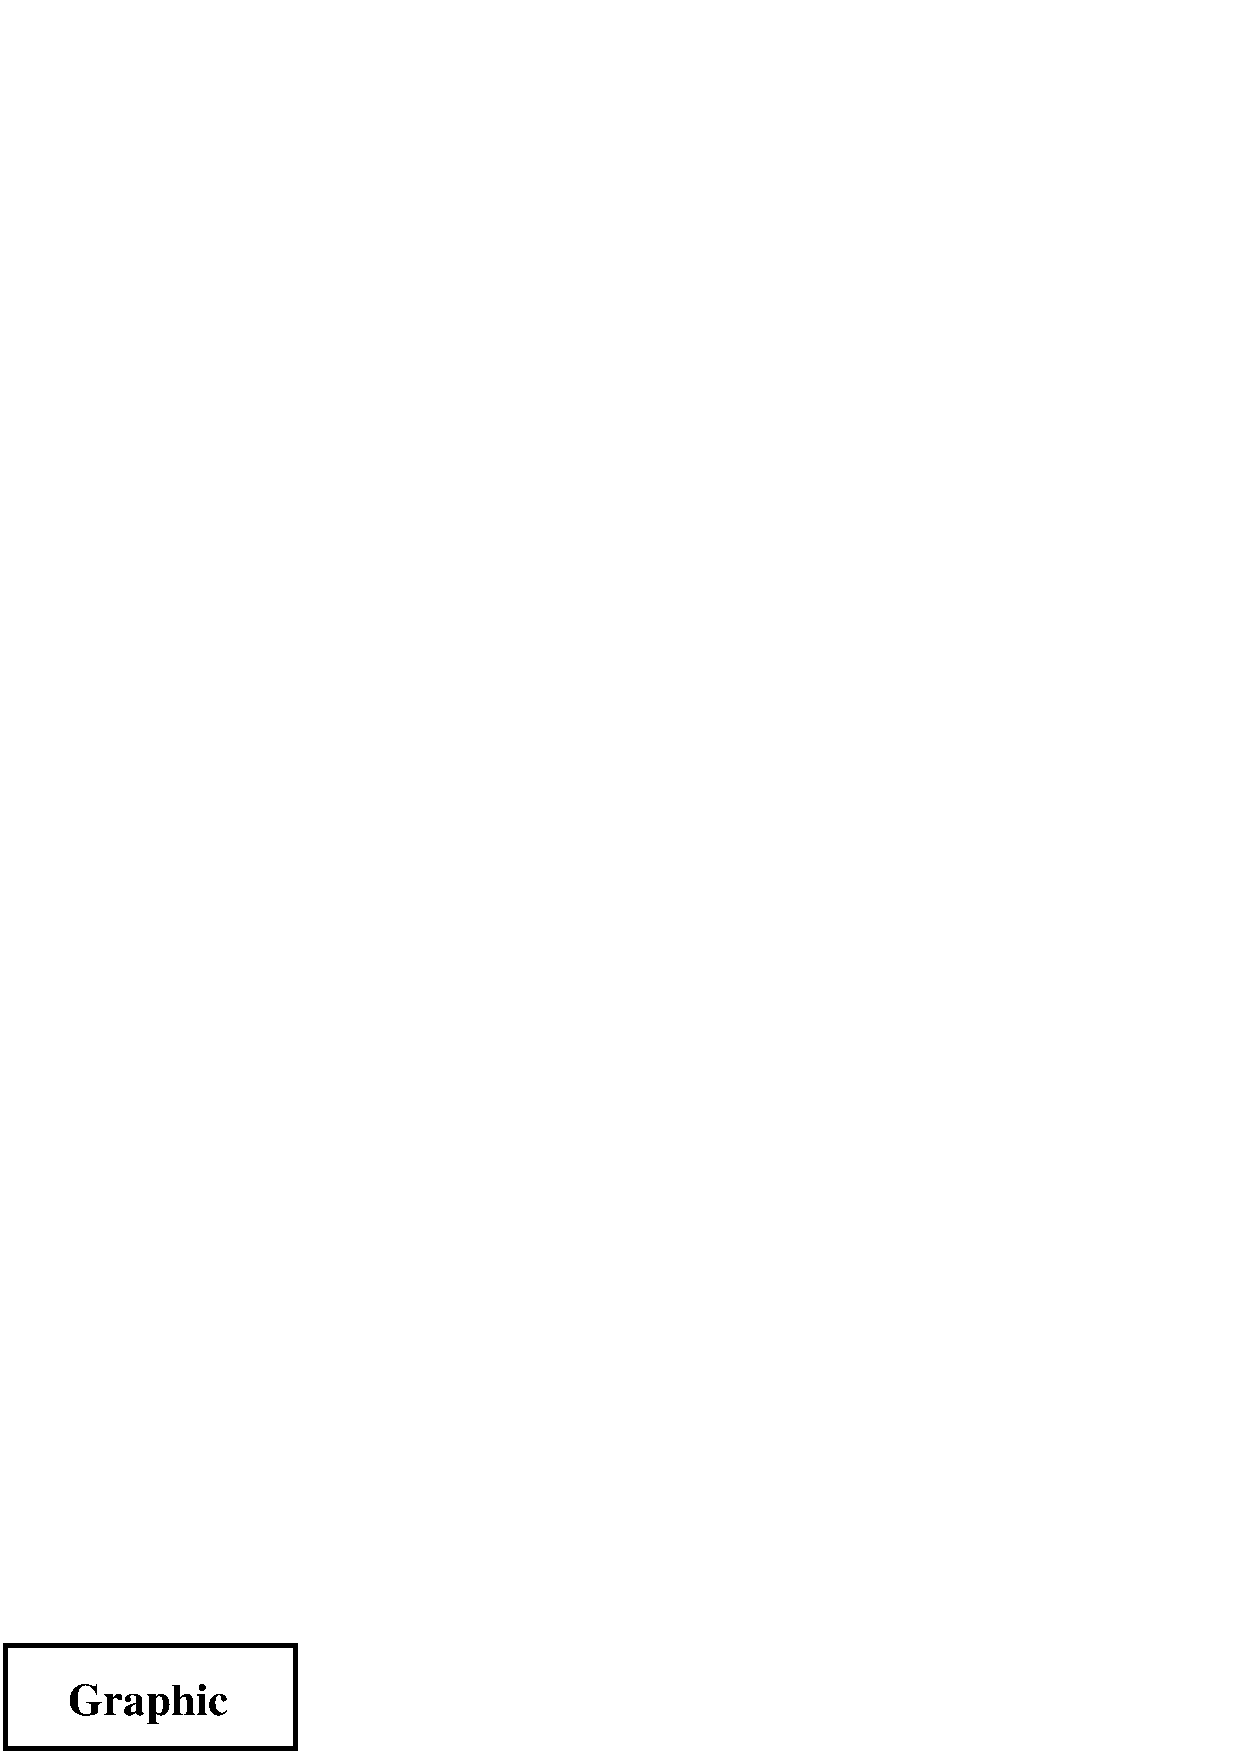
\includegraphics[width=1in]{graphic}% 
	\hspace{1in}% 
	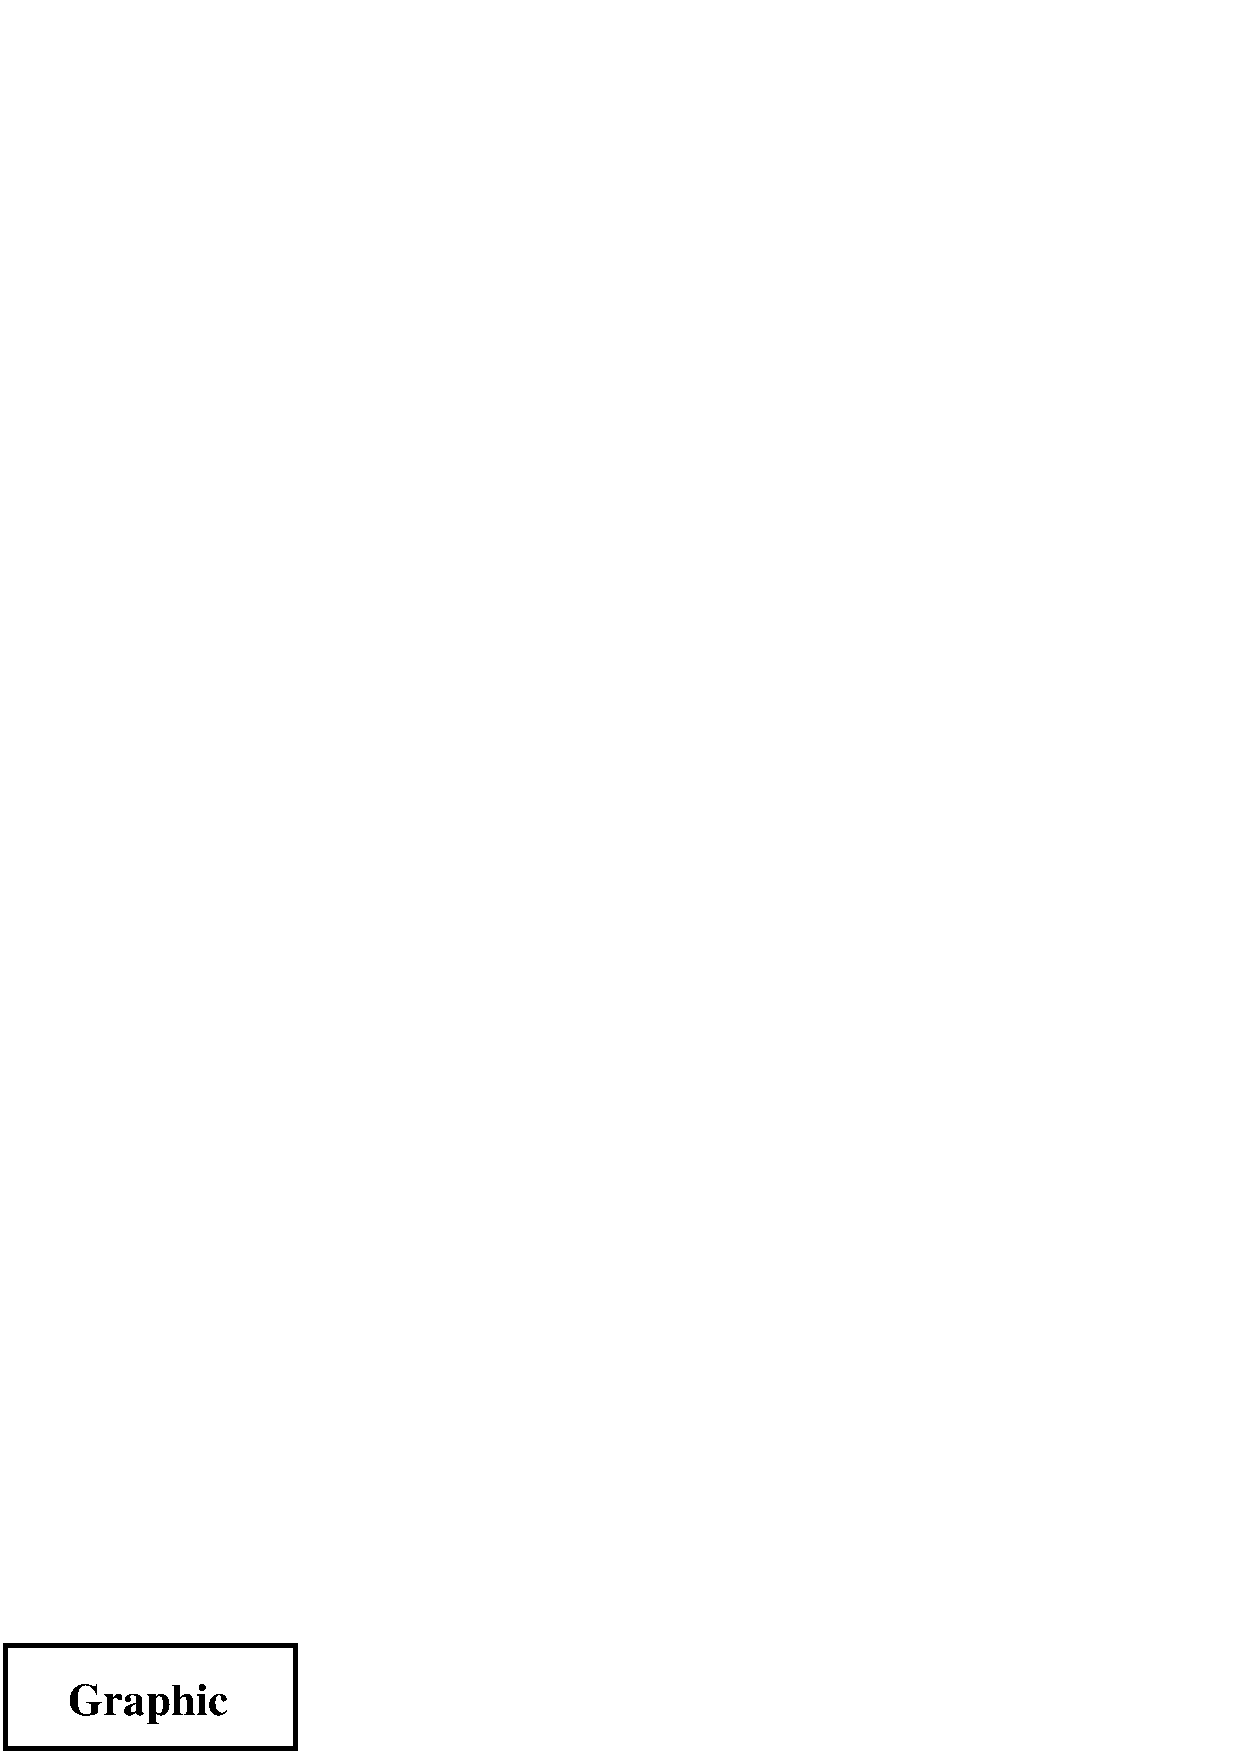
\includegraphics[width=2in]{graphic} 
	\caption{一个 figure 环境中的两幅图像} 
\end{figure}
\end{lstlisting}
会得到如图~\ref{fig:sidegraphics}~的并列图形。
该图形宽度为4英寸(第一幅图1英寸,\cmd{hspace}1英寸,第二幅图2英寸),居中放置。
其中的 \cmd{hspace} 命令可用 \cmd{hfill} 来代替,
这会将图形推向页面的两端边界(见第~\ref{ssec:hspace}~节)。

\begin{figure} 
	\centering 
	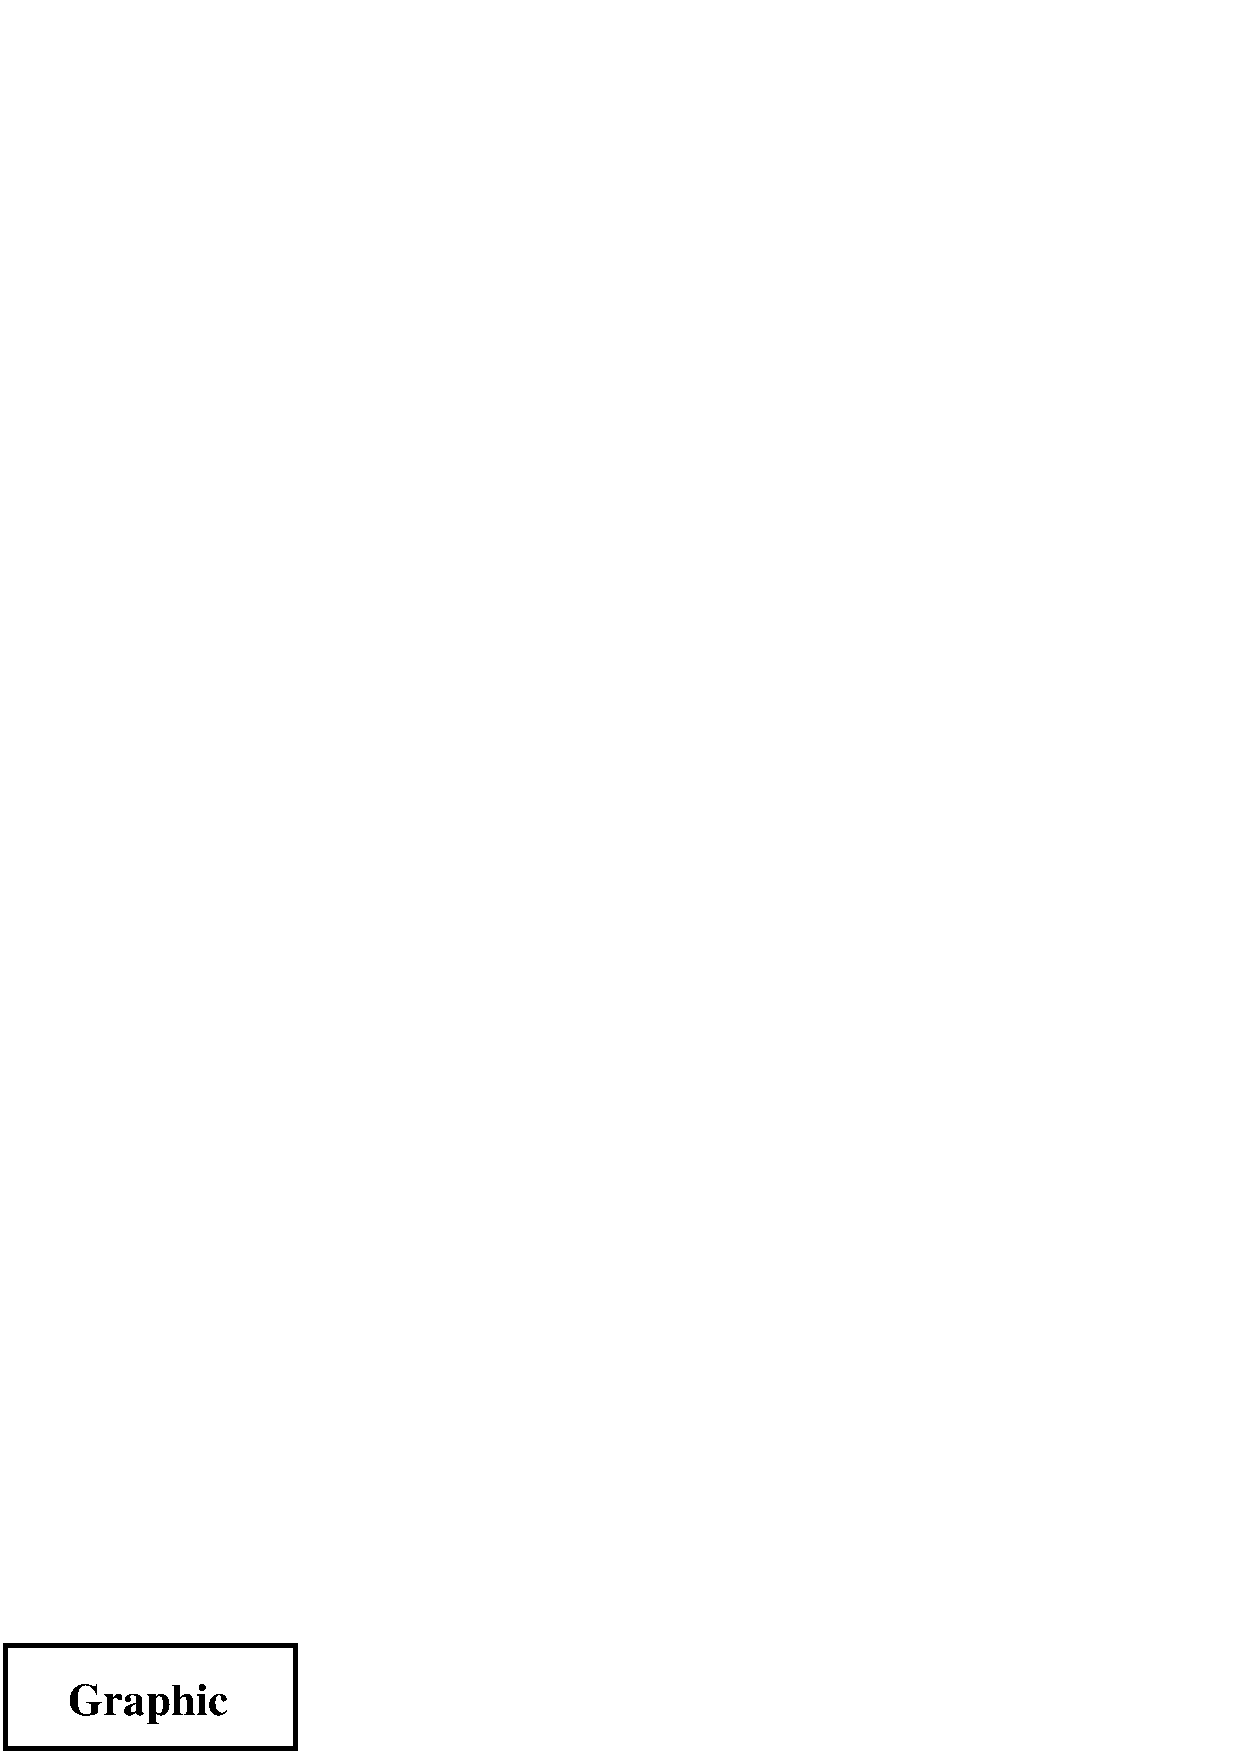
\includegraphics[width=1in]{graphic}% 
	\hspace{1in}% 
	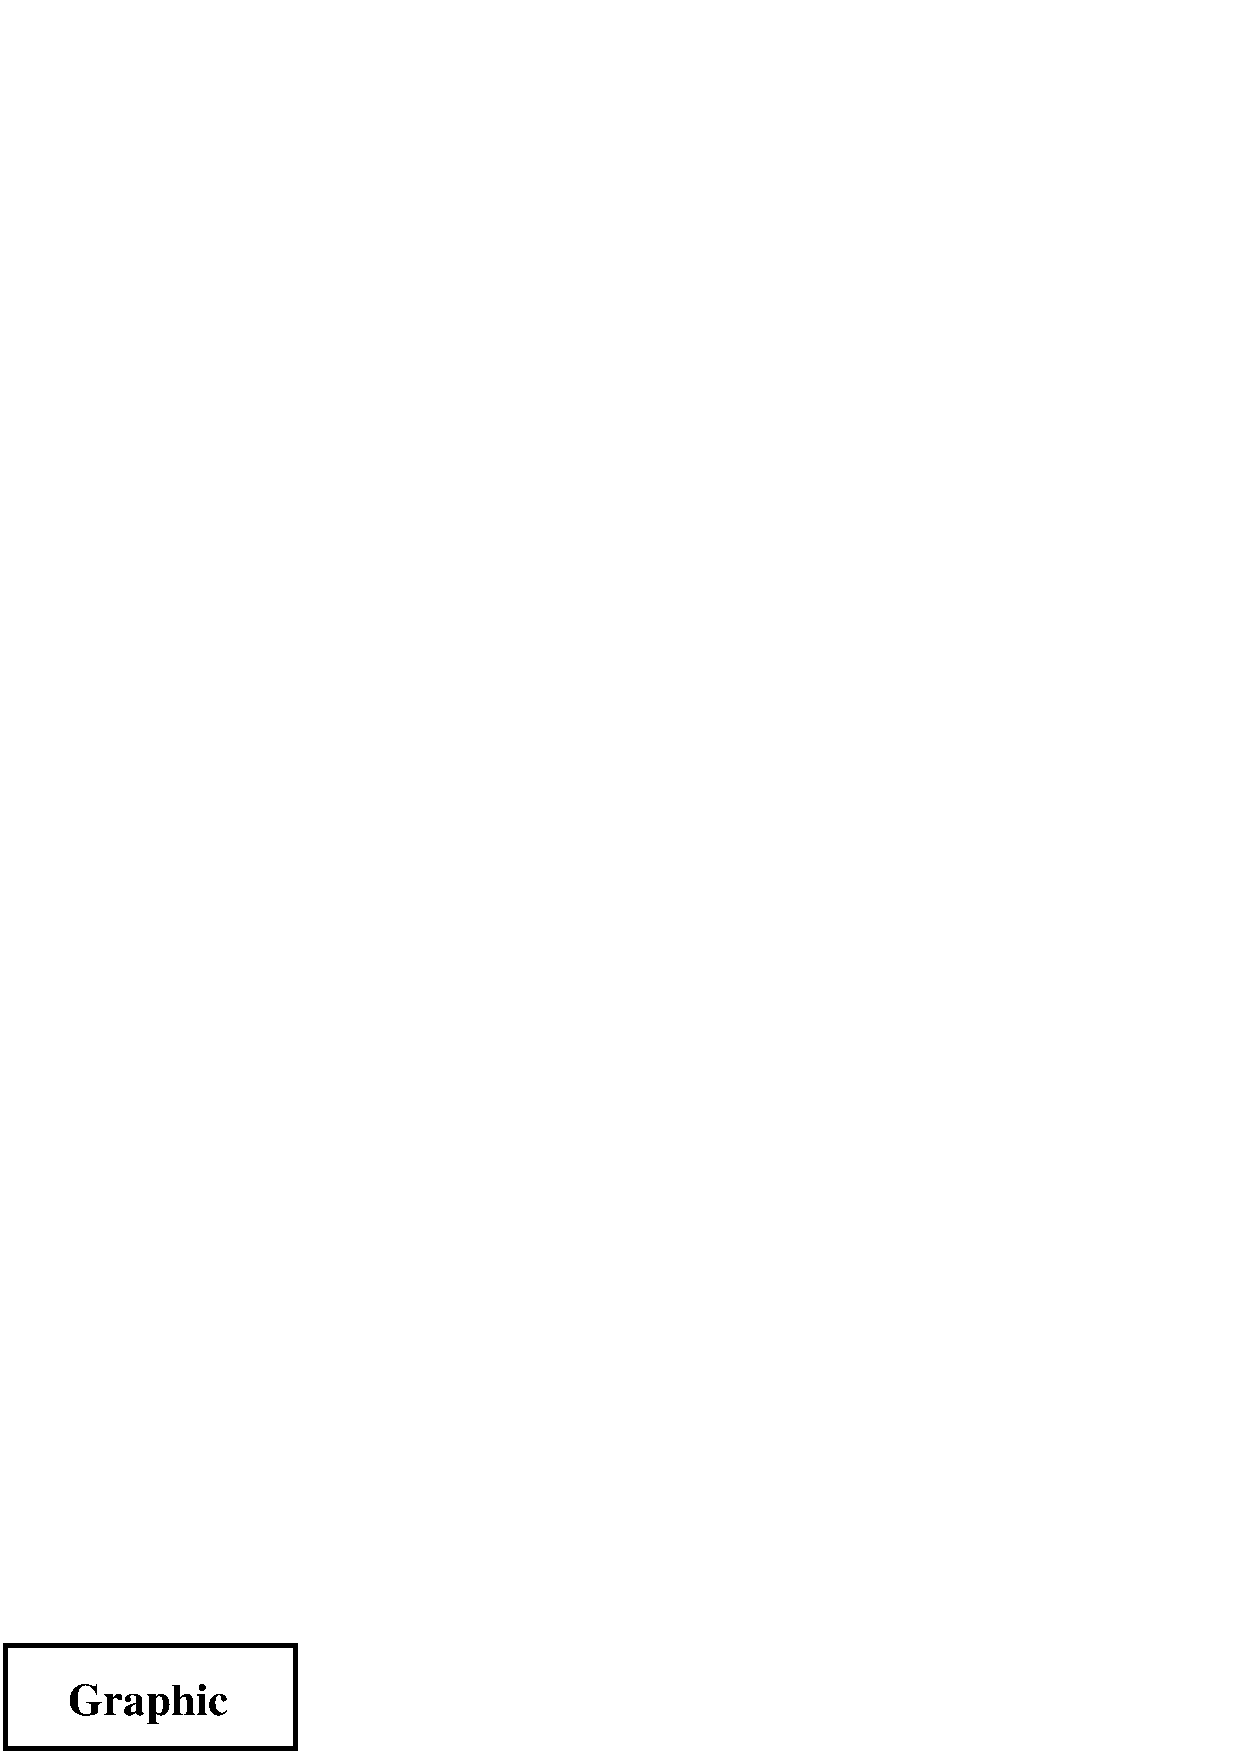
\includegraphics[width=2in]{graphic} 
	\caption{一个 \env{figure} 环境中的两幅图像}\label{fig:sidegraphics}
\end{figure}

\subsubsection{使用并列的小页环境}

Placing the \includegraphics commands inside minipage environments provides
the user more control over the graphics’ vertical placement. For example
\begin{figure}
	\centering
	\begin{minipage}[c]{0.5\linewidth}
		\centering 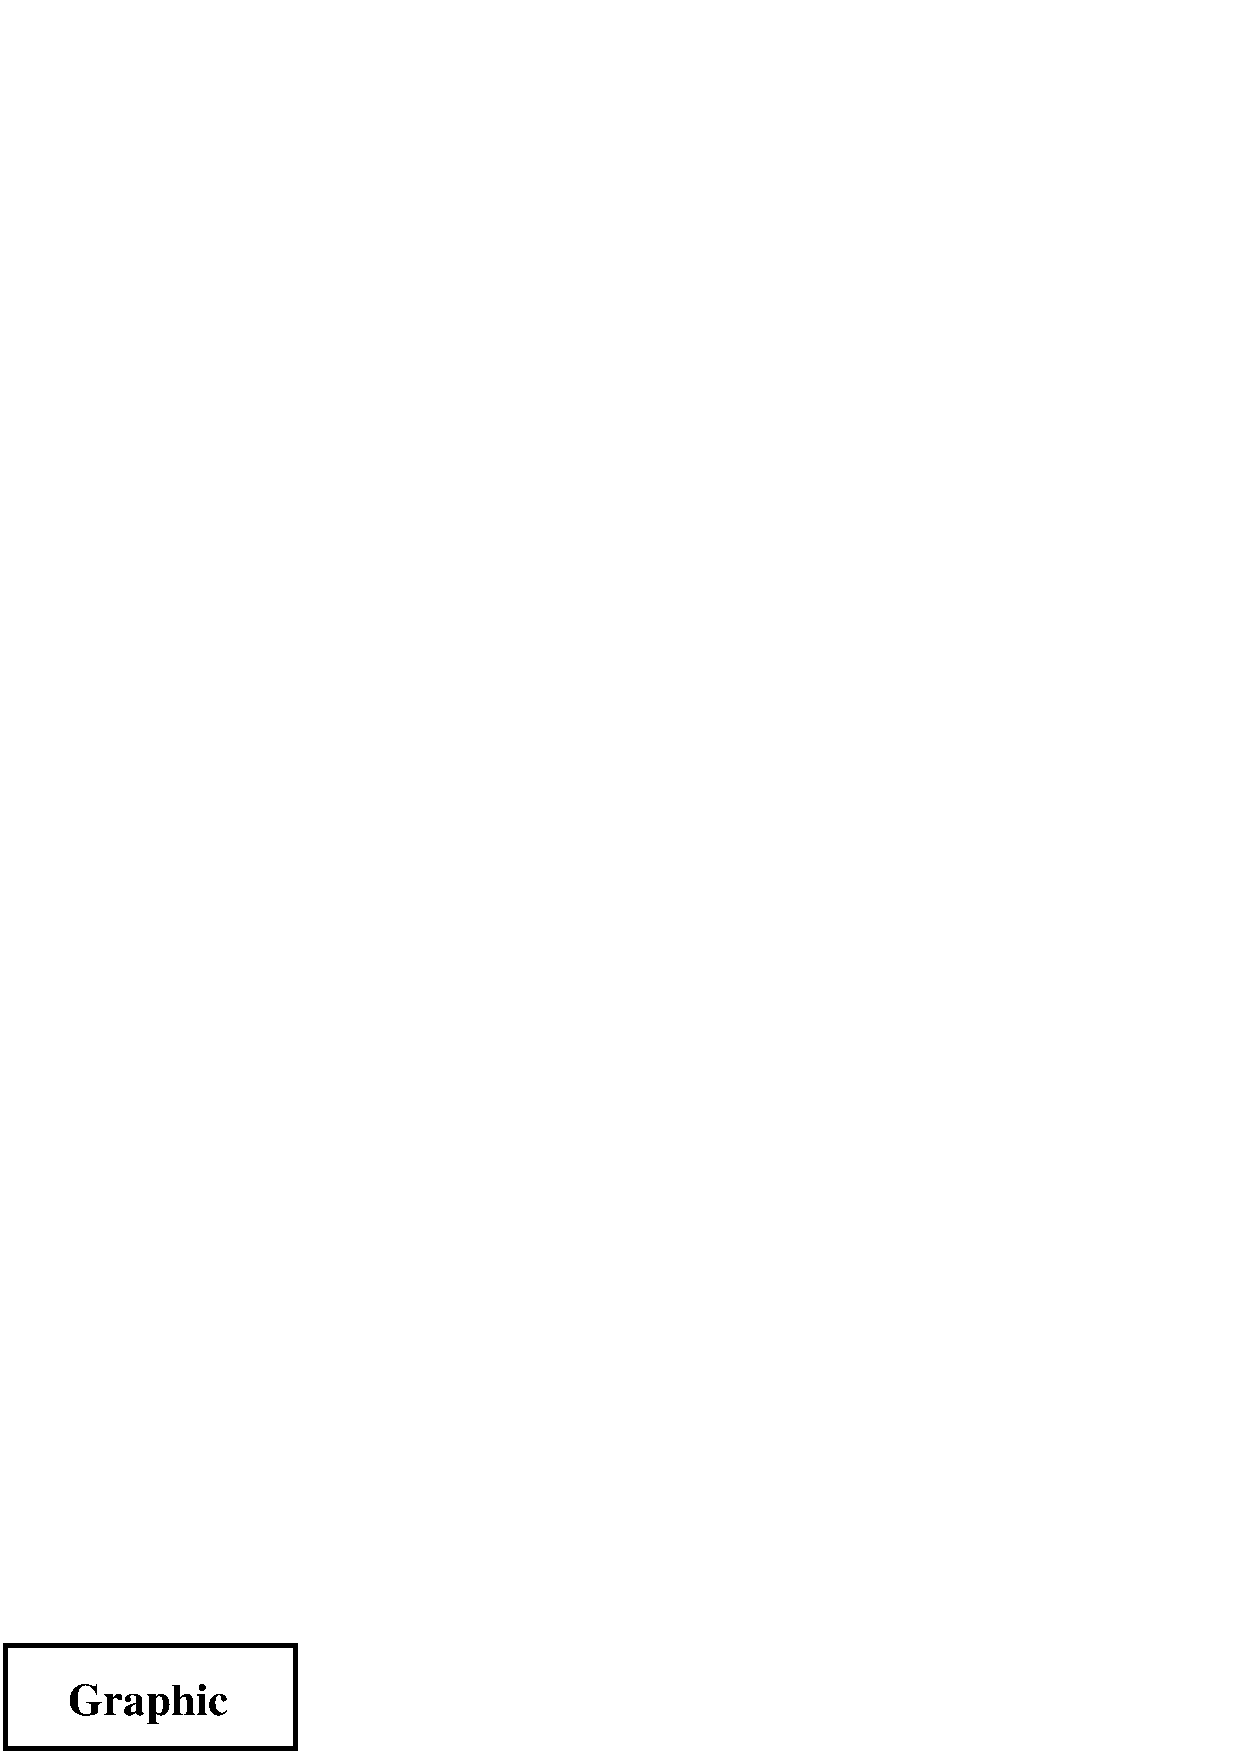
\includegraphics[width=1in]{graphic}
	\end{minipage}%
	\begin{minipage}[c]{0.5\linewidth}
		\centering 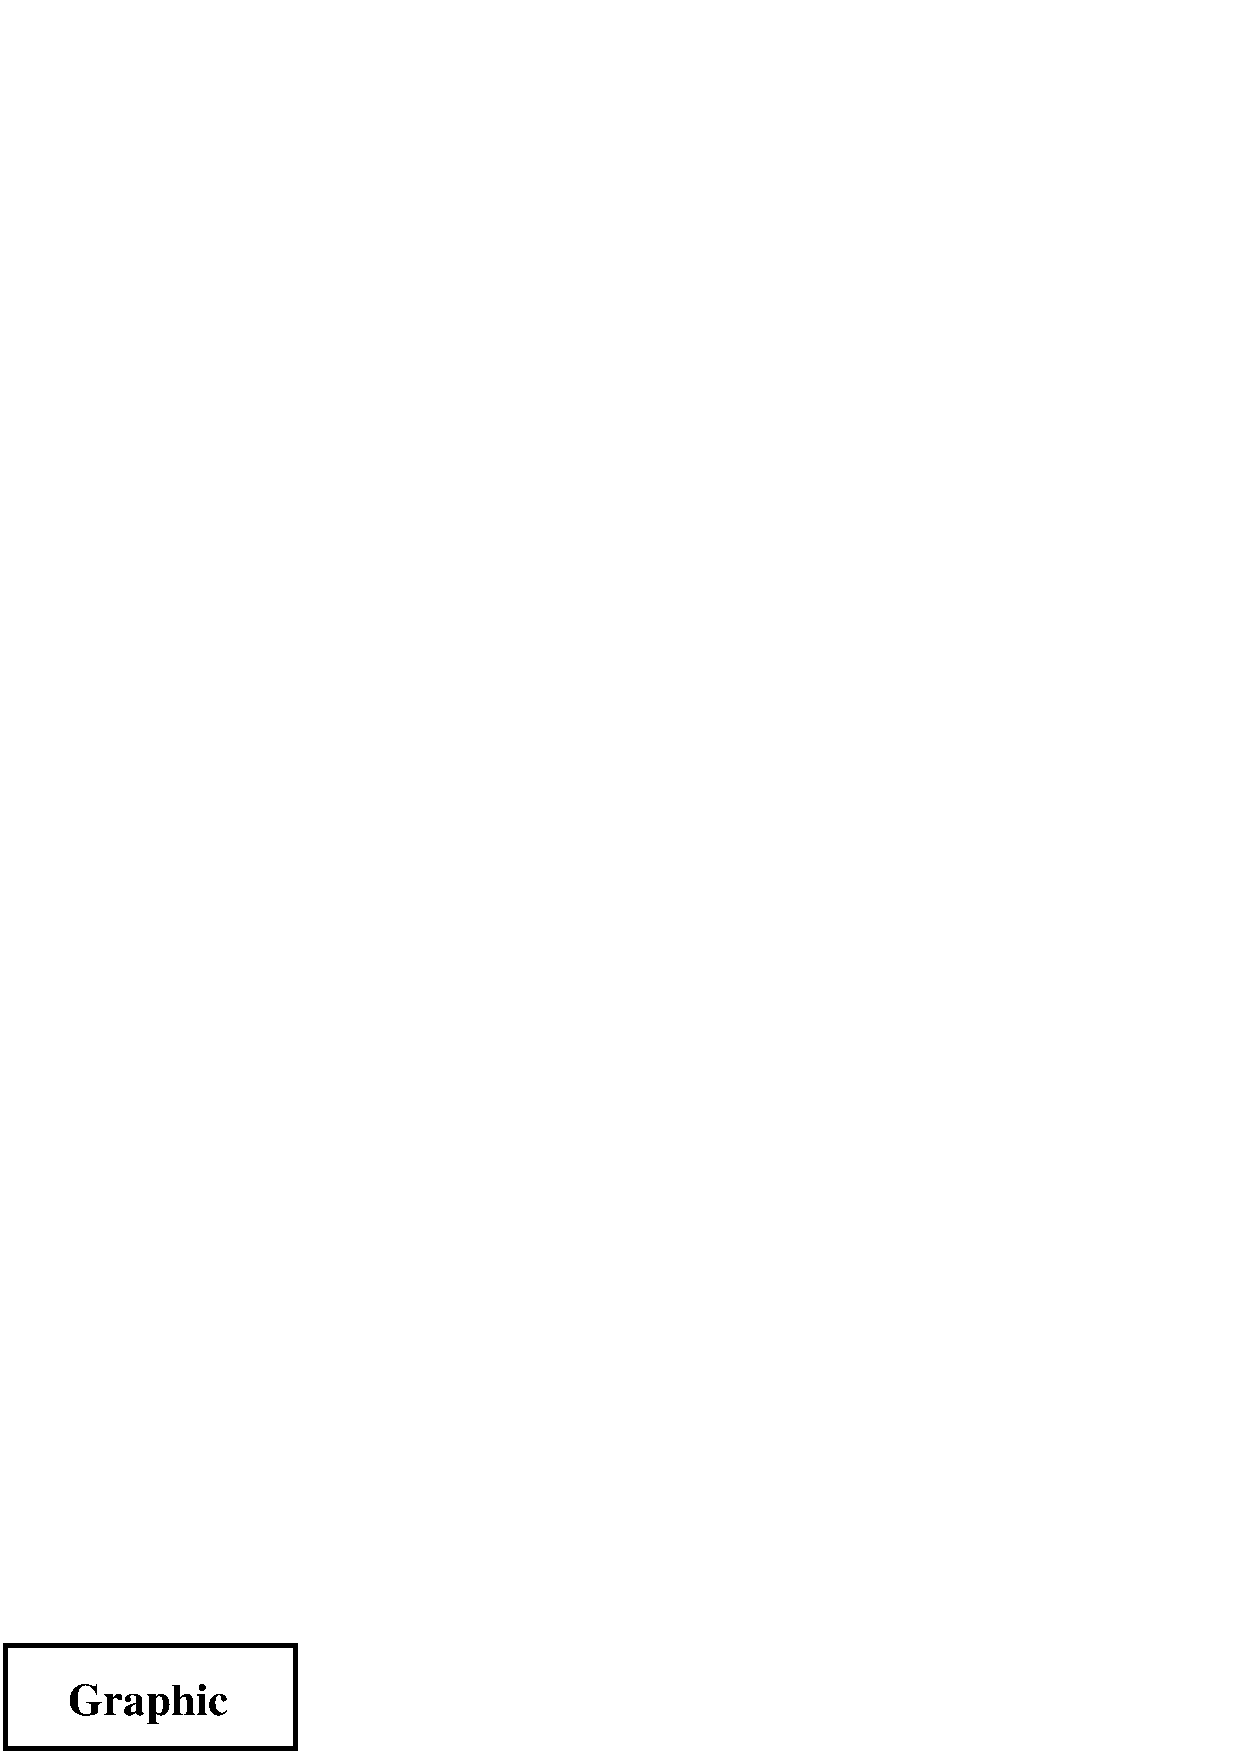
\includegraphics[width=2in]{graphic}
	\end{minipage}
	\caption{Centers Aligned Vertically}
\end{figure}
produces Figure 62, which has vertically-centered graphics.

将 \cmd{includegraphics} 命令放到小页环境中可以更好地控制图形的对齐方式。例如:
\begin{lstlisting}
\begin{figure} 
	\centering 
	\begin{minipage}[c]{0.5\textwidth} 
		\centering 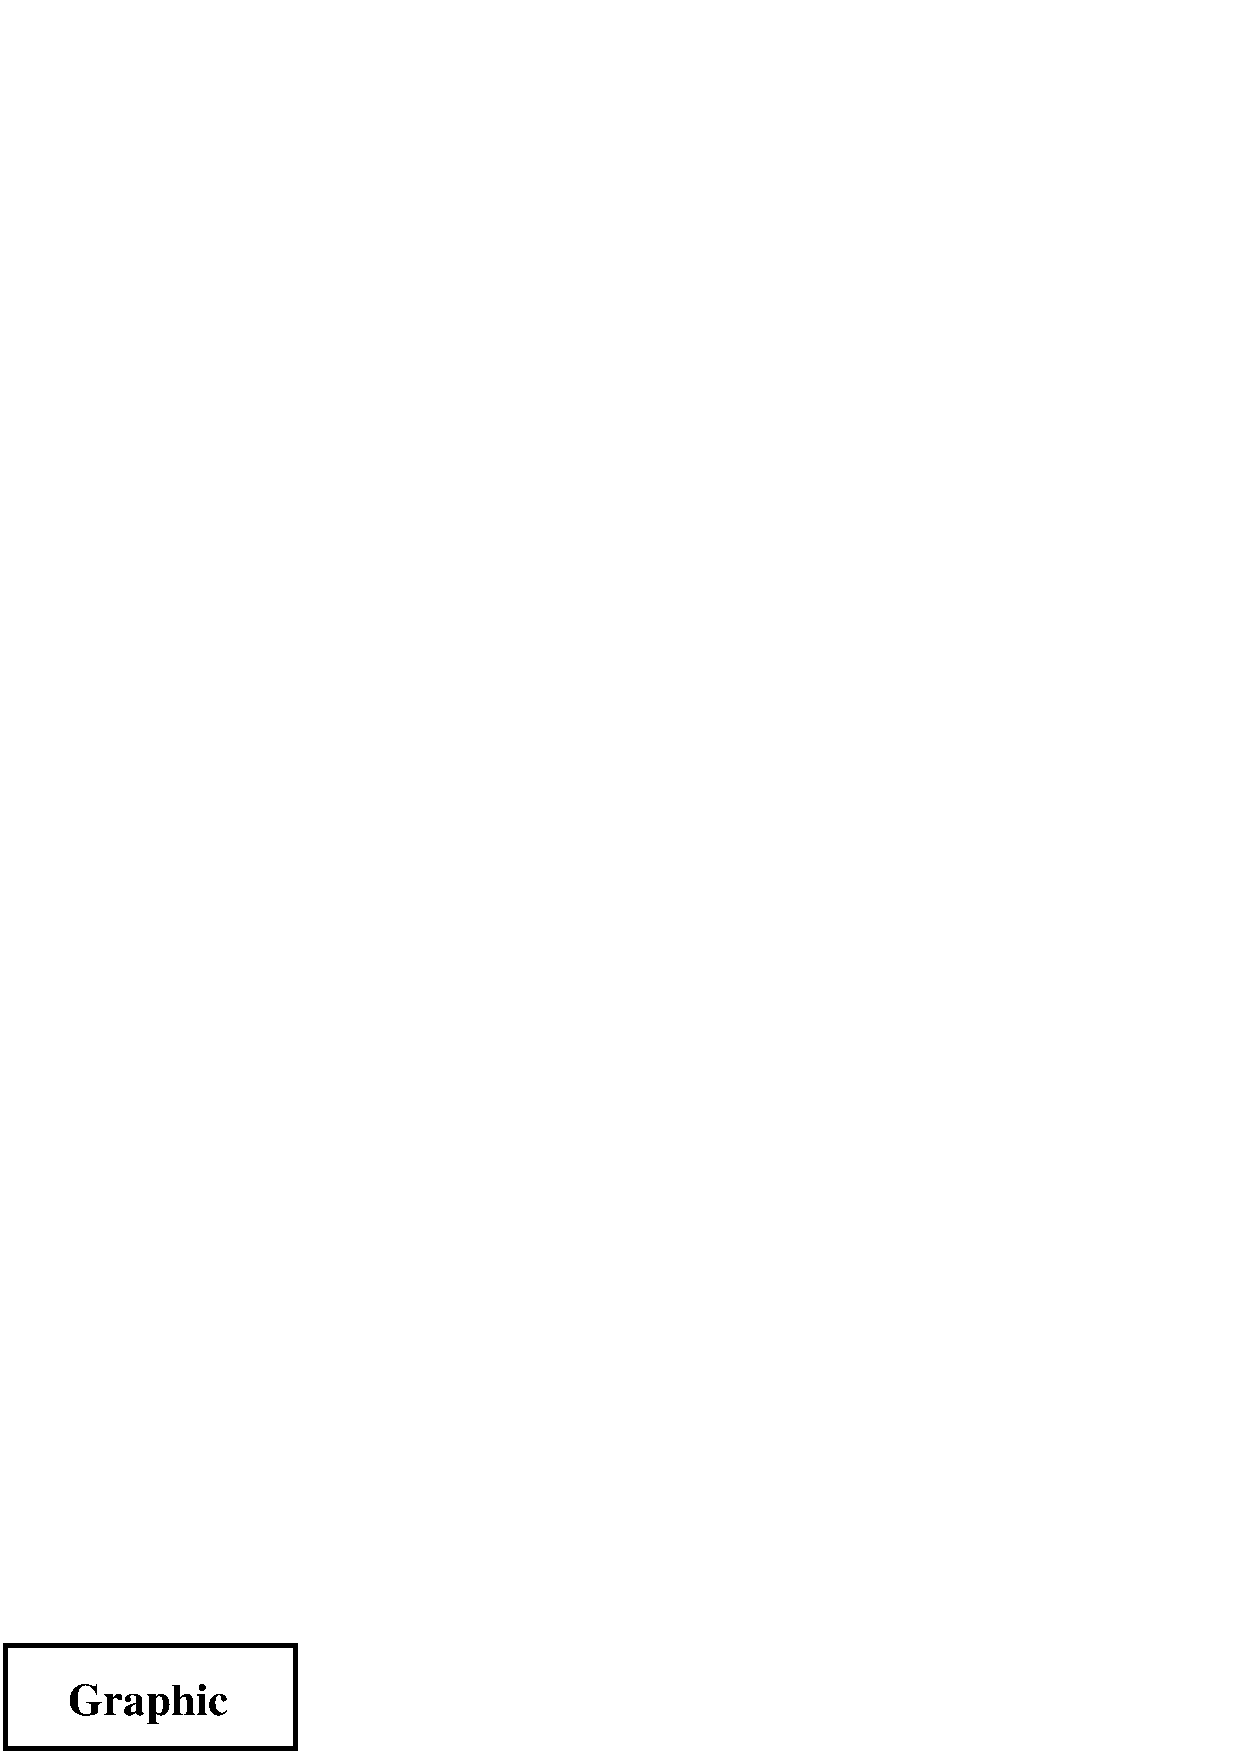
\includegraphics[width=1in]{graphic} 
	\end{minipage}% 
	\begin{minipage}[c]{0.5\textwidth} 
		\centering 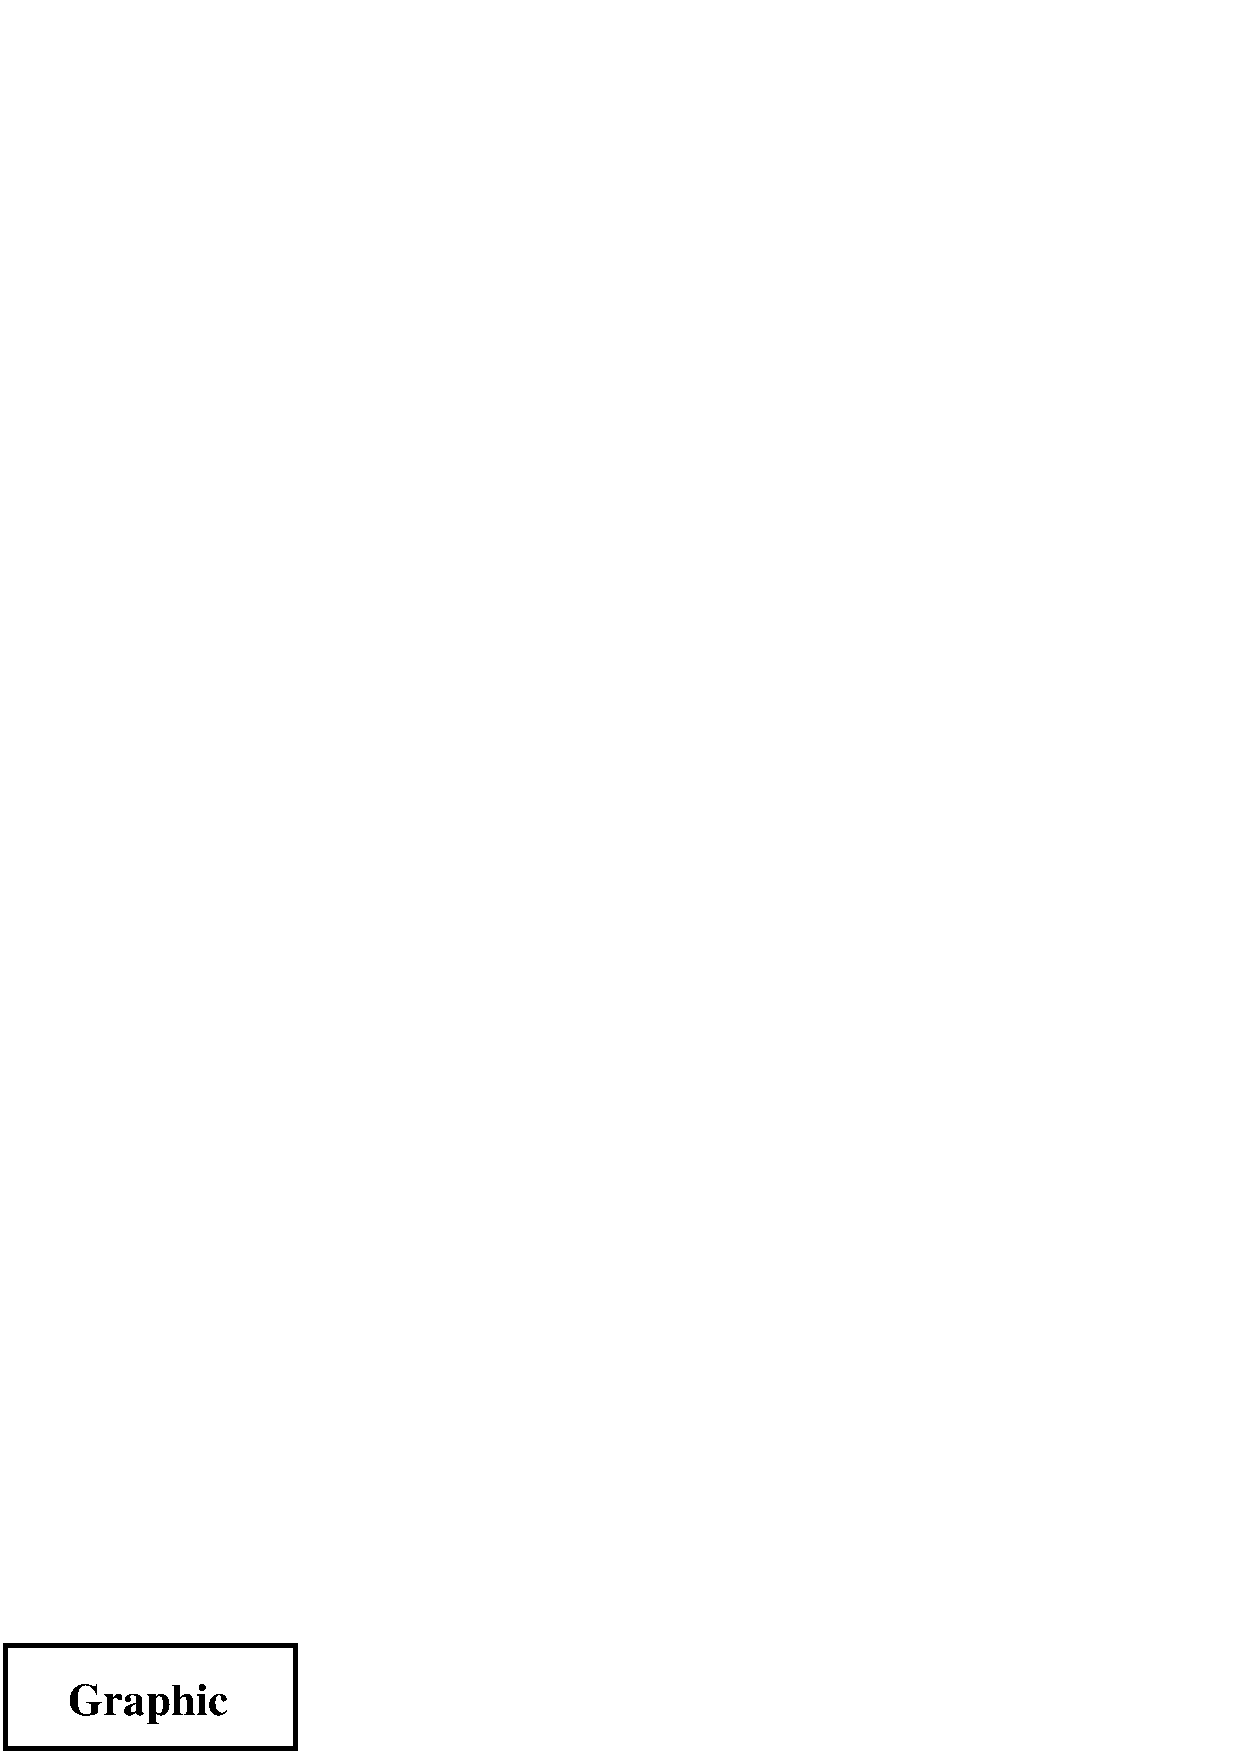
\includegraphics[width=2in]{graphic} 
	\end{minipage} 
	\caption{中间对齐的图像} 
\end{figure}
\end{lstlisting}
生成图~\ref{fig:minipagegraphics}~,其中的图形是中间对齐的。

\begin{figure} 
	\centering 
	\begin{minipage}[c]{0.5\textwidth} 
		\centering 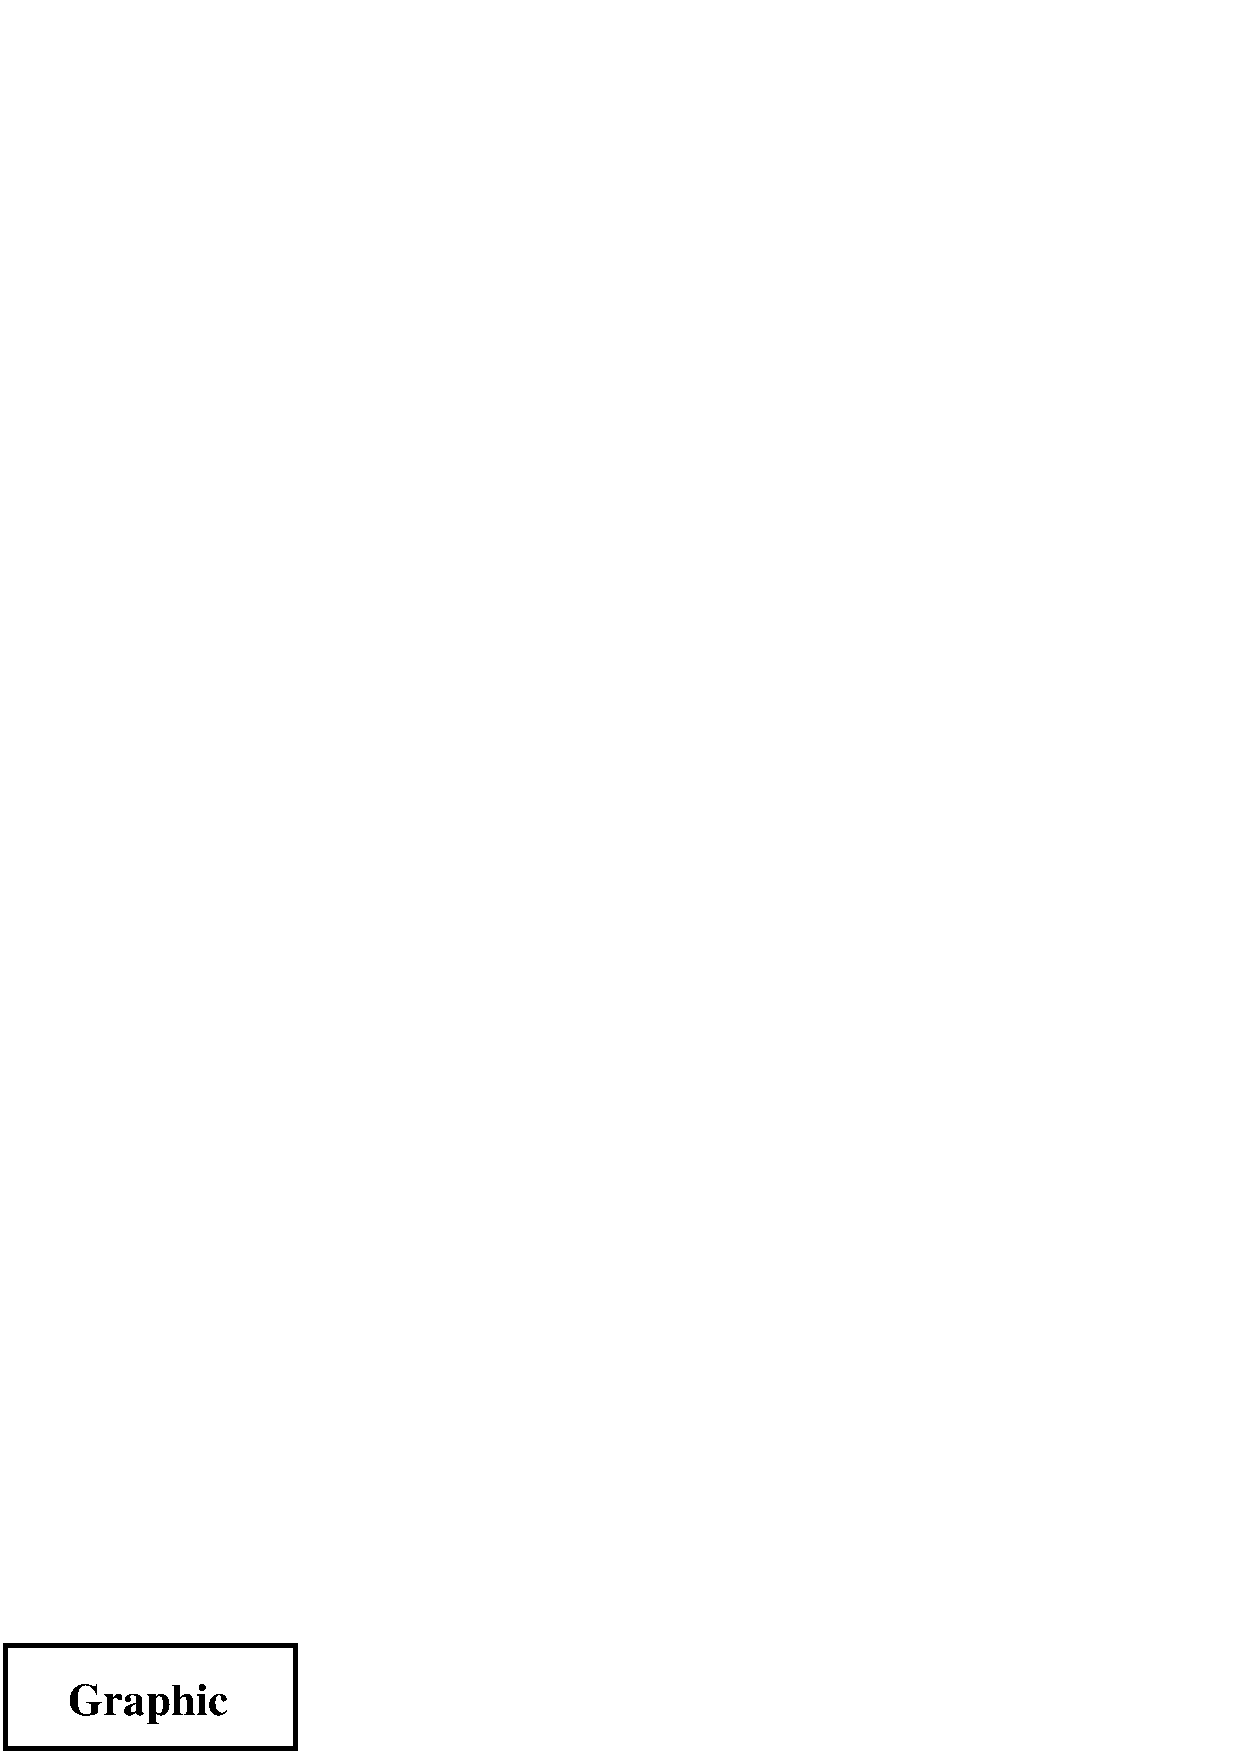
\includegraphics[width=1in]{graphic} 
	\end{minipage}% 
	\begin{minipage}[c]{0.5\textwidth} 
		\centering 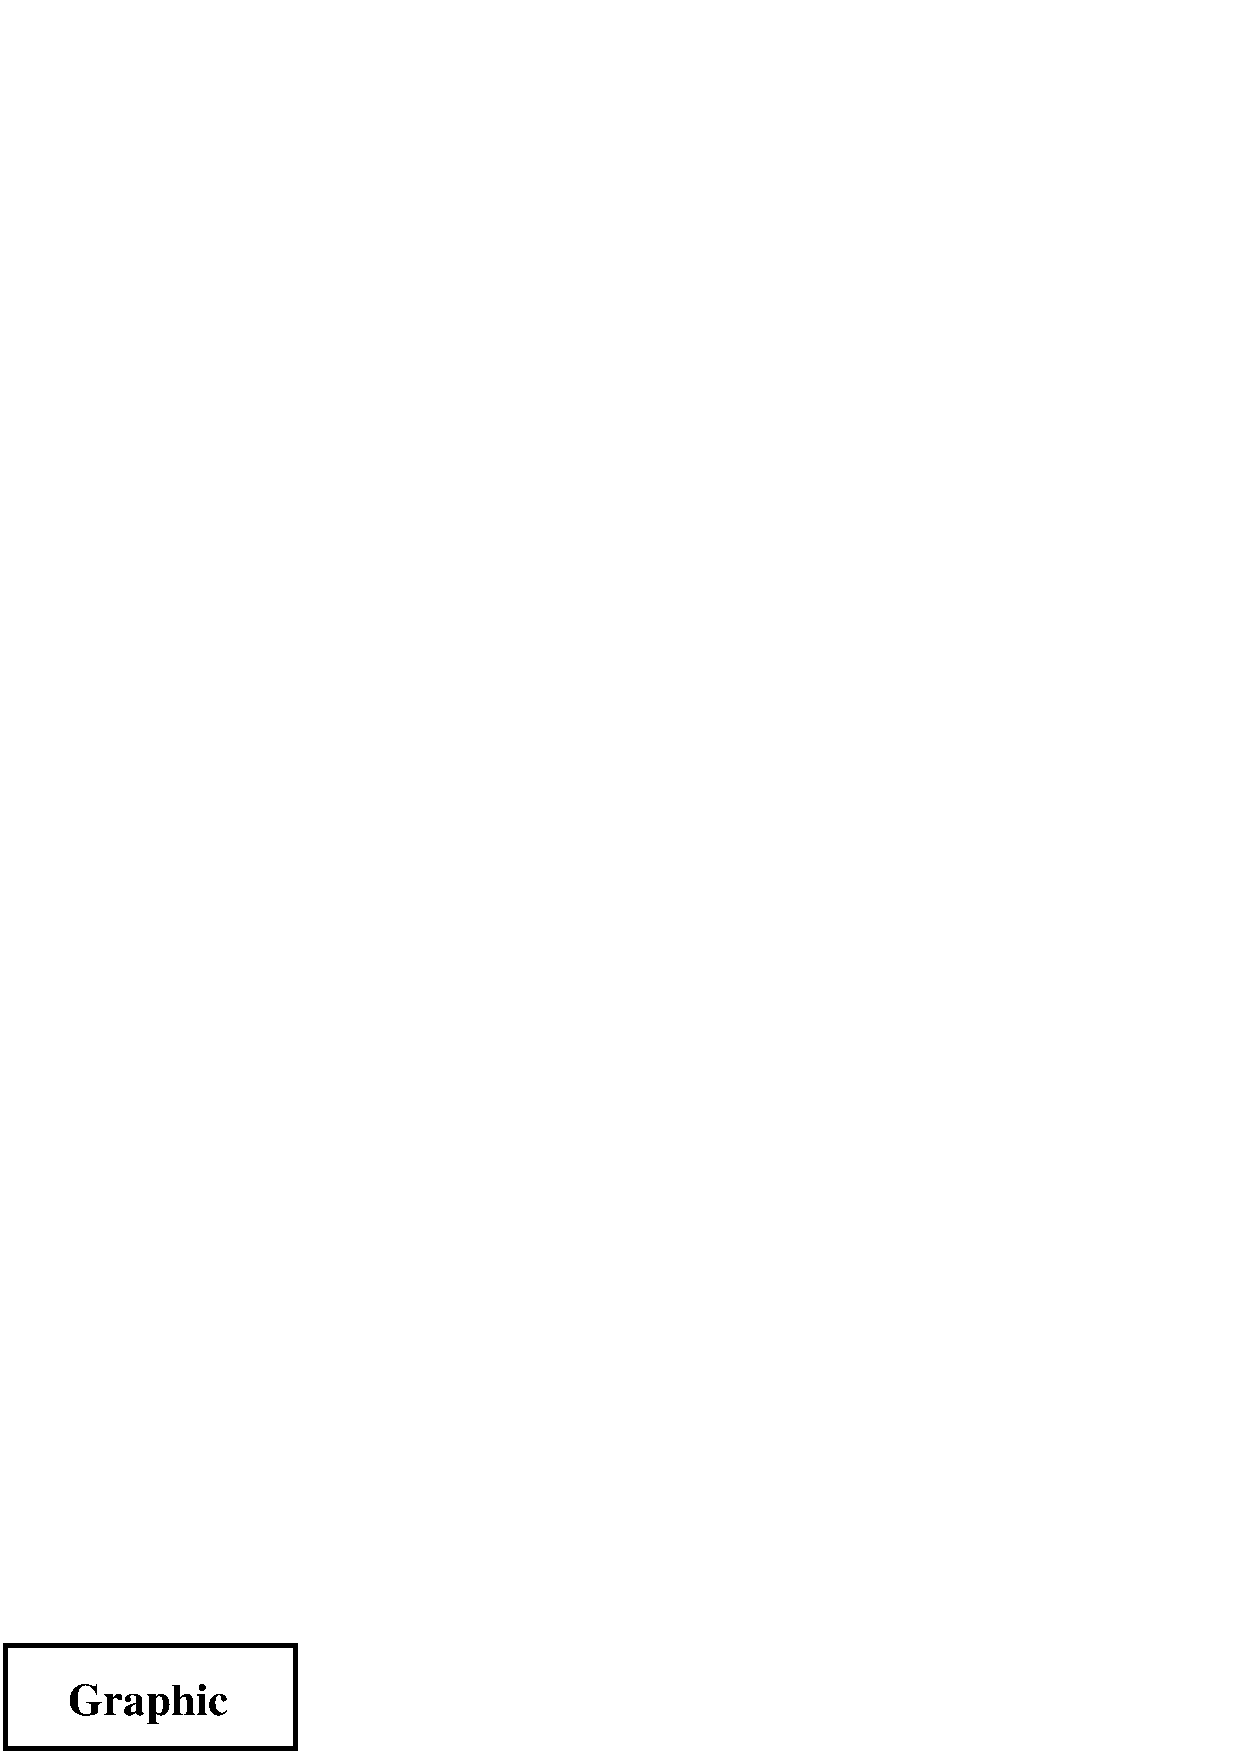
\includegraphics[width=2in]{graphic} 
	\end{minipage} 
	\caption{中间对齐的图像} \label{fig:minipagegraphics}
\end{figure}

对于这个例子,需要注意以下几点:
\begin{itemize}
	\item 如同其它的 \LaTeX{} 对象一样,小页在放置时,它的参考点和当前基线对齐。
	缺省情况下小页使用 \opt{[c]} 选项,将参考点置于其竖直方向的中点。
	选项 \opt{[t]} 将参考点置于小页顶行的基线上,
	而选项 \opt{[b]} 将参考点置于小页底行的基线上(参见第~\ref{ssec:minivalign}~节)。
	
	\item 在第一个 \cmdM{end}{minipage} 后面的 \texttt{\%} 防止在两个小页之间多一个空格
	(参见第~\ref{ssec:hspace} 节)。
	
	\item 当几个并列小页的宽度之和没有达到 $1.0\text{\cmd{textwidth}}$ 时,
	可用 \cmd{hspace} 或 \cmd{hfill} 来确定水平间距,详见第~\ref{ssec:hspace}~节。
\end{itemize}


\subsection{并列的浮动图形}\label{ssec:sidefigure}

在上一节中,通过在一个图形环境中使用多个小页环境得到一个由多幅图像组成的浮动图形。
若将  \cmd{caption} 命令放到每个小页环境中,则每个小页环境自己就变成浮动图形。例如:
\begin{lstlisting}
\begin{figure}
	\centering
	%%----start of first figure----
	\begin{minipage}[t]{0.4\linewidth}
		\centering
		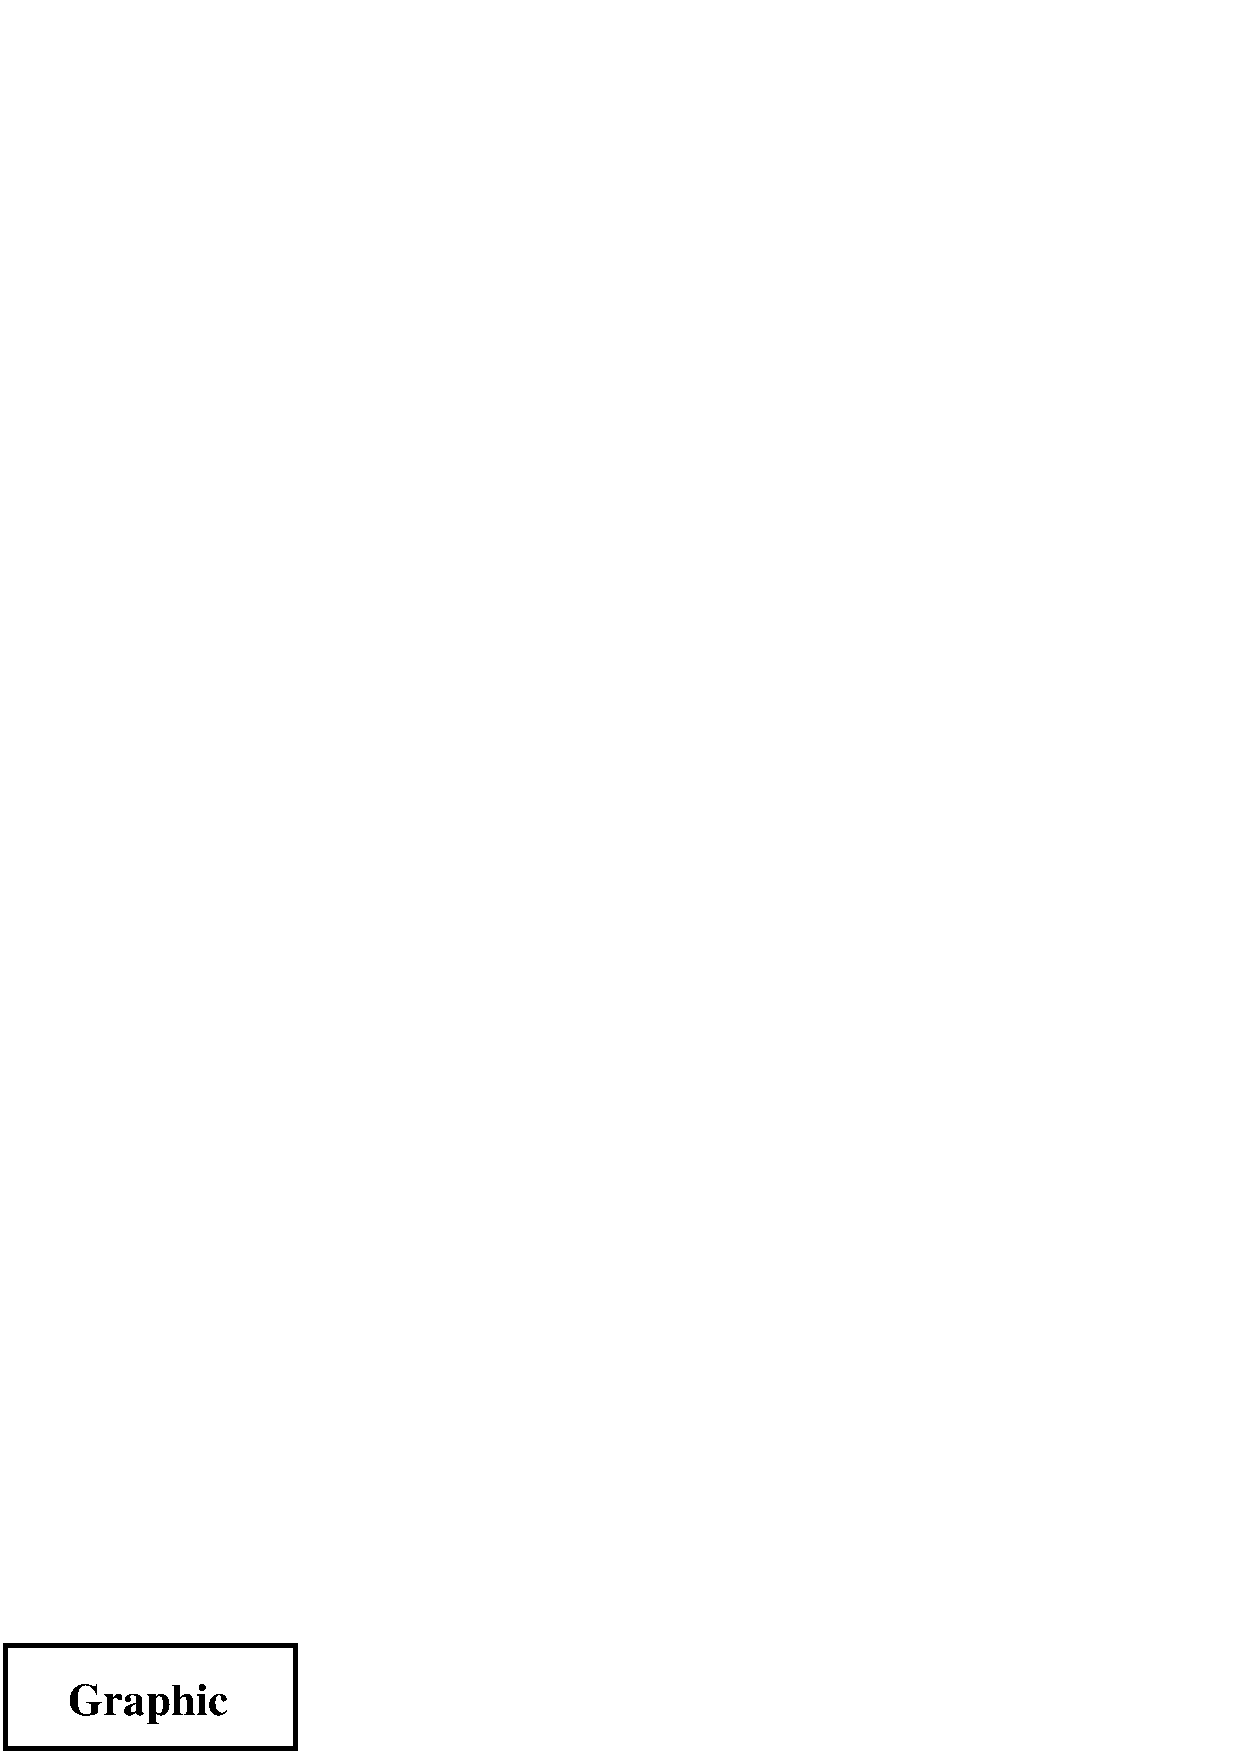
\includegraphics[width=1in]{graphic}
		\caption{Small Box} \label{fig:side:a}
	\end{minipage}%
	\hspace{1cm}%
	%%----start of second figure----
	\begin{minipage}[t]{0.4\linewidth}
		\centering
		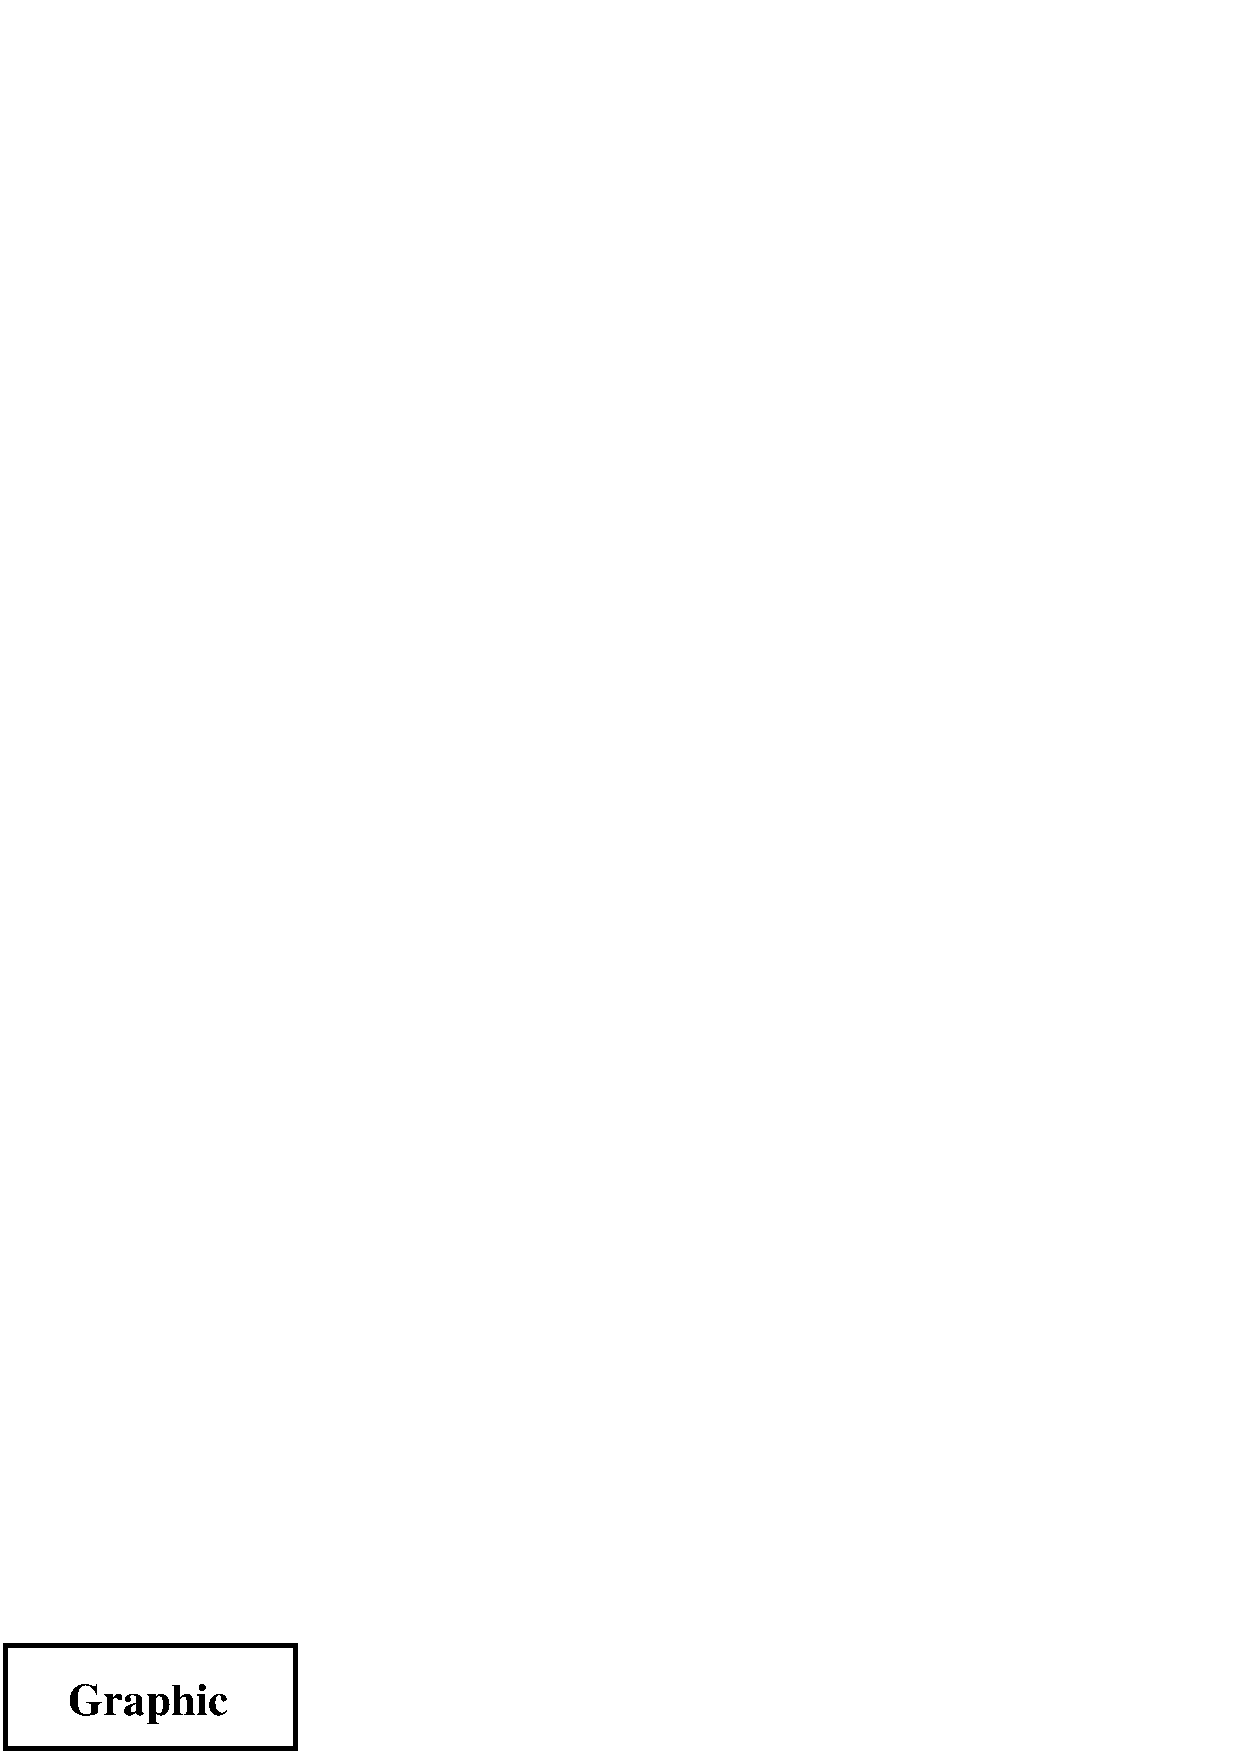
\includegraphics[width=1.5in]{graphic}
		\caption{Big Box} \label{fig:side:b}
	\end{minipage}
\end{figure}
\end{lstlisting}
生成图~\ref{fig:side:a}~和~\ref{fig:side:b}。

\begin{figure}
	\centering
	%%----start of first figure----
	\begin{minipage}[t]{0.4\linewidth}
		\centering
		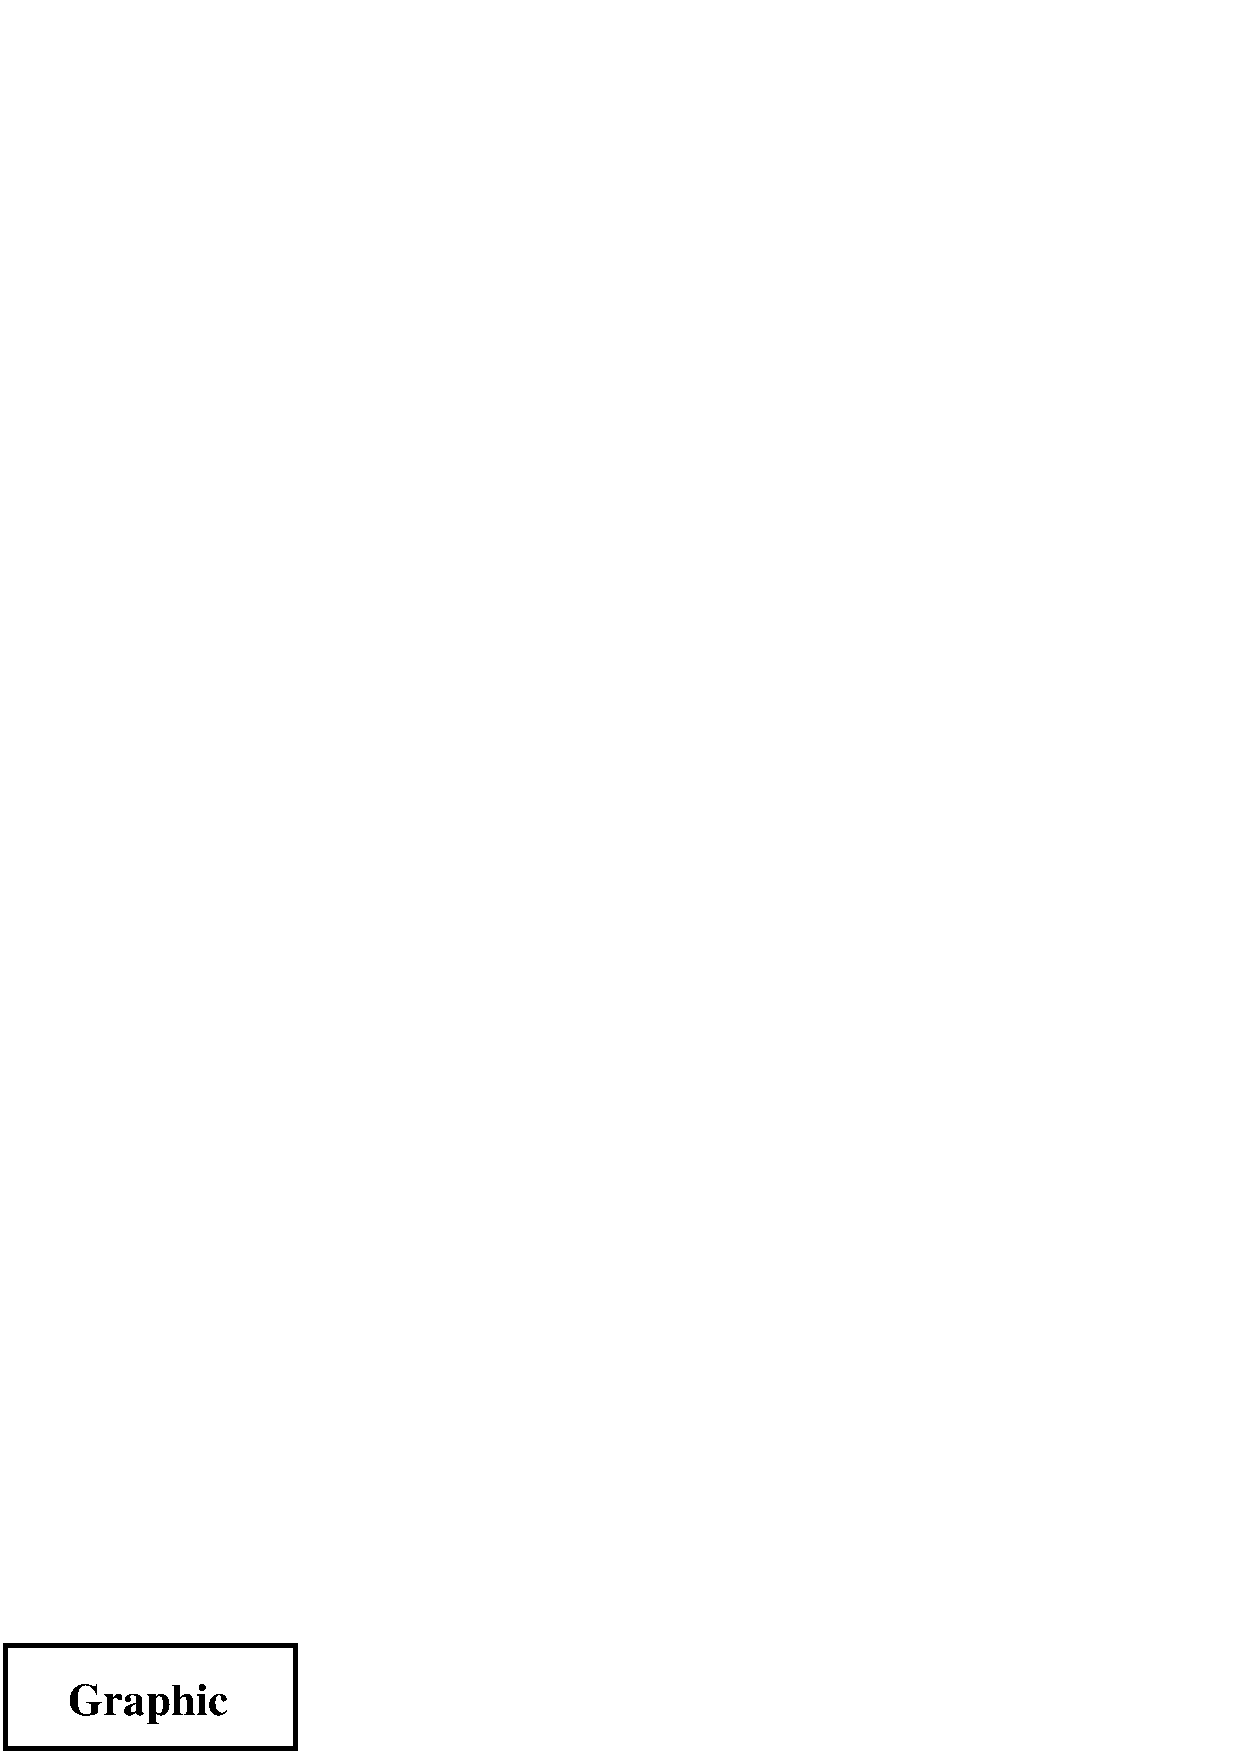
\includegraphics[width=1in]{graphic}
		\caption{Small Box} \label{fig:side:a}
	\end{minipage}%
	\hspace{1cm}%
	%%----start of second figure----
	\begin{minipage}[t]{0.4\linewidth}
		\centering
		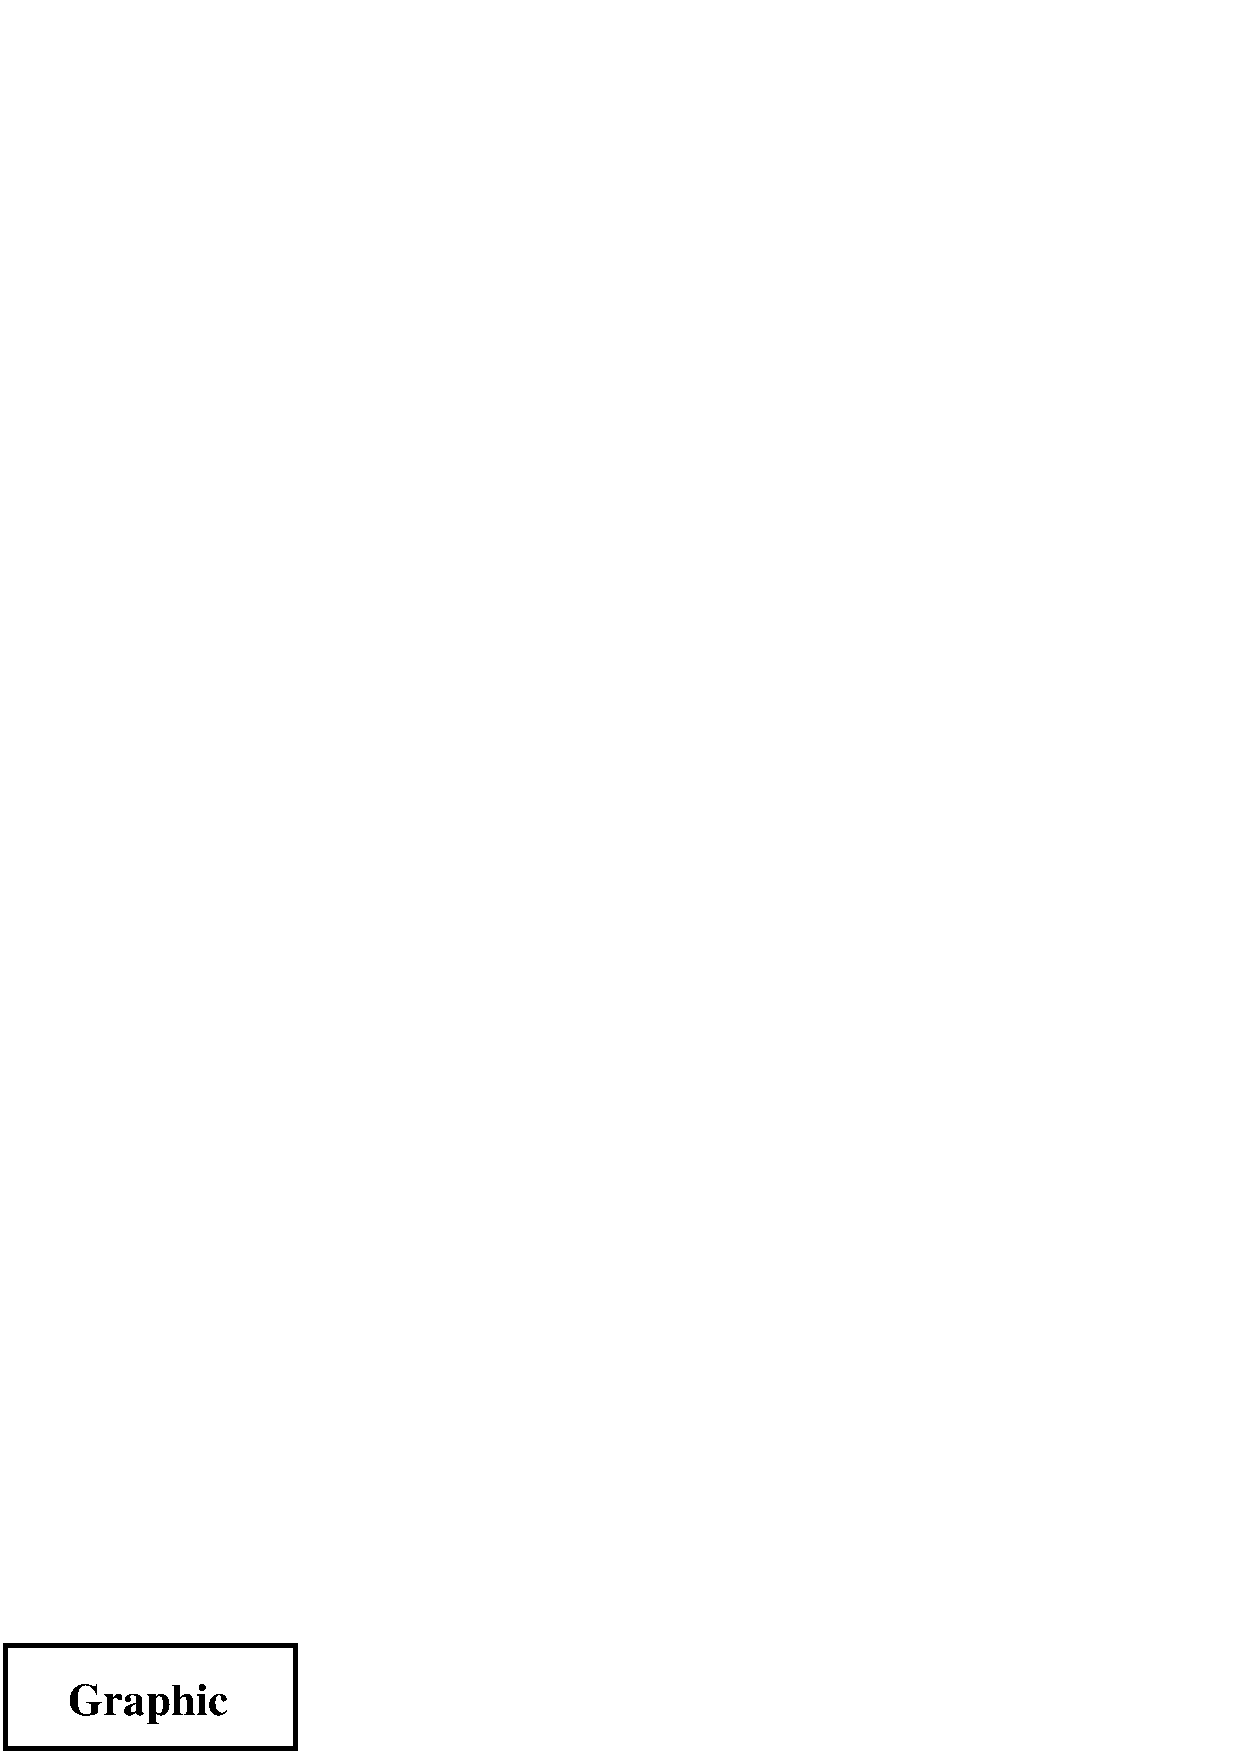
\includegraphics[width=1.5in]{graphic}
		\caption{Big Box} \label{fig:side:b}
	\end{minipage}
\end{figure}

关于该例子有几个注记:
\begin{itemize}
	\item 尽管上面的命令只使用了一个 \env{figure} 环境,
	但由于每个小页中都包含 \cmd{caption} 命令,所以仍然得到两个浮动图形。
	
	\item 两个放置图像的小页环境宽度为 \env{figure} 环境宽度的 $40\percent$,
	之间有1厘米的水平间距。
	(注意,在 \cmdM{end}{minipage} 和 \cmdM{hspace}{1cm} 之后的注释会阻止额外的空格,
	从而确保了间距正好是1厘米。)
	
	默认情况下,图形标题的宽度就是小页环境的宽度。
	使用1厘米的水平间距是为了确保标题之间有空白(无论对长标题还是很宽的图像)。
	
	此外,标题的宽度也可以用 \pkg{caption} 宏包的 \opt{margin} 或 \opt{width} 关键字进行控制
	(参见表~\ref{tab:caption-formatopt})。
	
	\item 紧接着 \cmdM{begin{figure} 的 \cmd{centering} 命令使得两个小页以及之间的空白在 \env{figure} 环境中居中放置。
		
	\item 小页内部的 \cmd{centering} 命令使得图像在小页环境内部居中放置。
\end{itemize}

\subsection{并列的子图形}\label{ssec:sidesubfigure}

在某些情况下,有时会希望将并列的图形组成一组,同时其中的每一幅图都保持其独立性。
\pkgi{subfig} 宏包的 \cmdi{subfloat} 命令(参见第~\ref{sec:subfig-pkg} 节)
可以将一组独立的图像作为一个 \env{figure} 环境中的子图。
例如:
\begin{lstlisting}
\usepackage{subfig}
...
\begin{figure}
	\centering
	%%----start of first subfigure----
	\subfloat[Small Box with a Long Caption]{
		\label{fig:subfig:a} %% label for first subfigure
		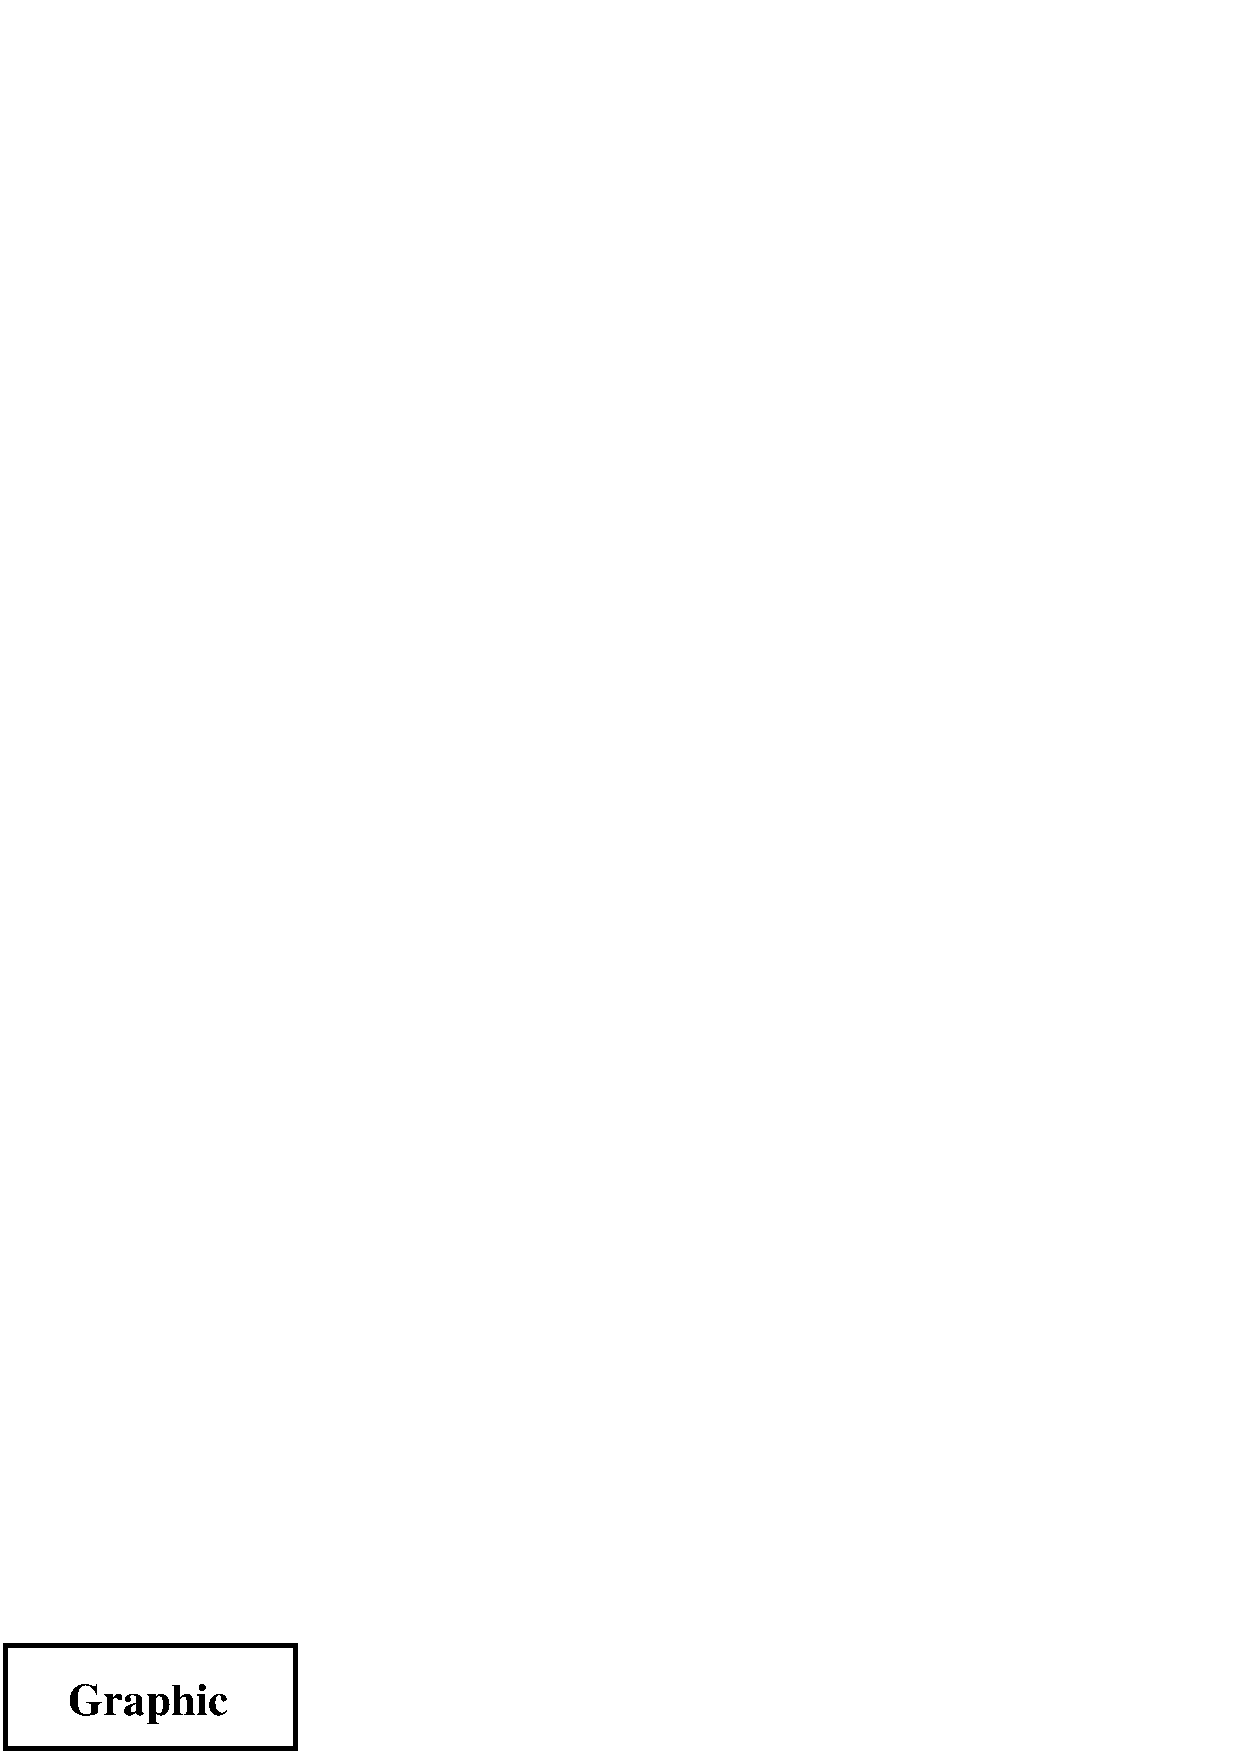
\includegraphics[width=1.0in]{graphic}}
	\hspace{1in}
	%%----start of second subfigure----
	\subfloat[Big Box]{
		\label{fig:subfig:b} %% label for second subfigure
		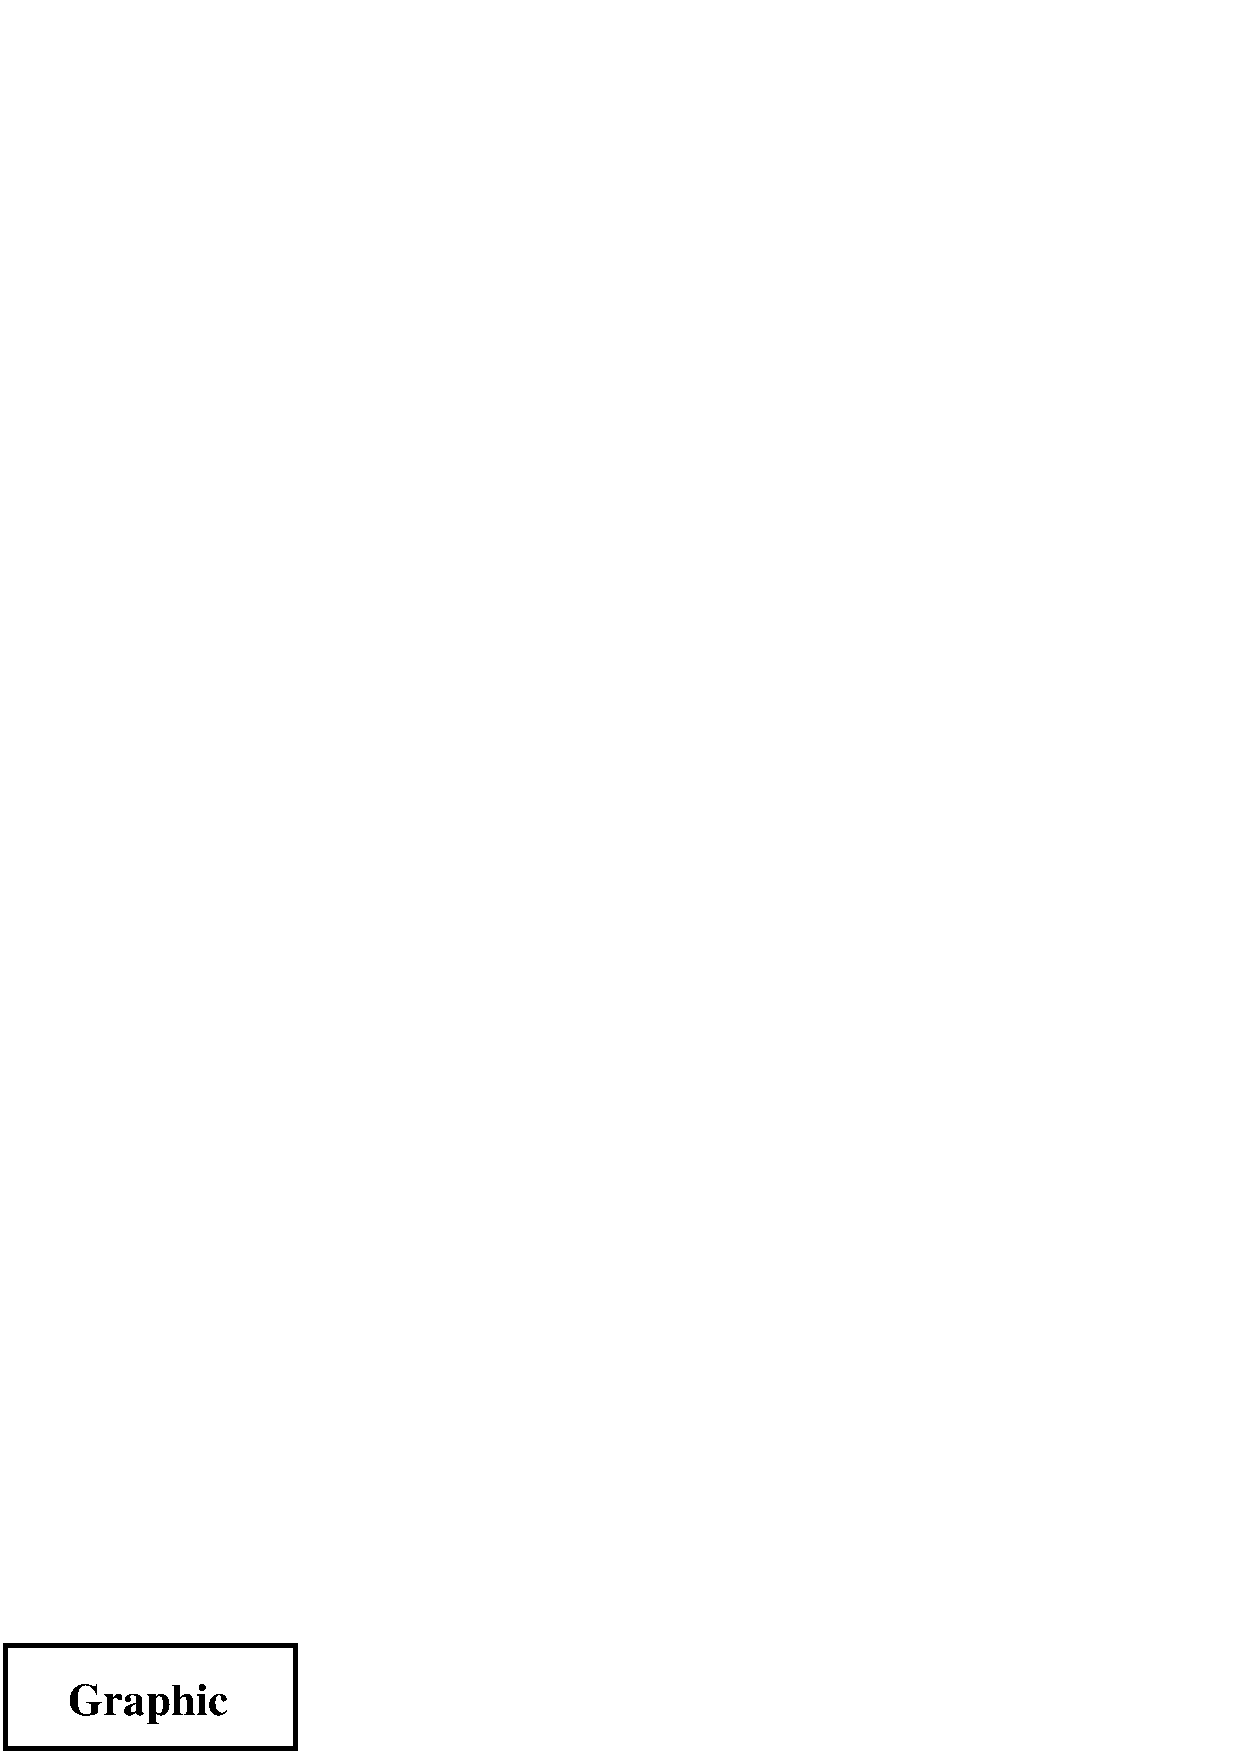
\includegraphics[width=1.5in]{graphic}}
	\caption{Two Subfigures}
	\label{fig:subfig} %% label for entire figure
\end{figure}
\end{lstlisting}
生成图~\ref{fig:subfig}。
表~\ref{tab:subfigref} 展示了用于如何引用图~\ref{fig:subfig} 中子图的命令。

\begin{figure}
	\centering
	%%----start of first subfigure----
	\subfloat[Small Box with a Long Caption]{
		\label{fig:subfig:a} %% label for first subfigure
		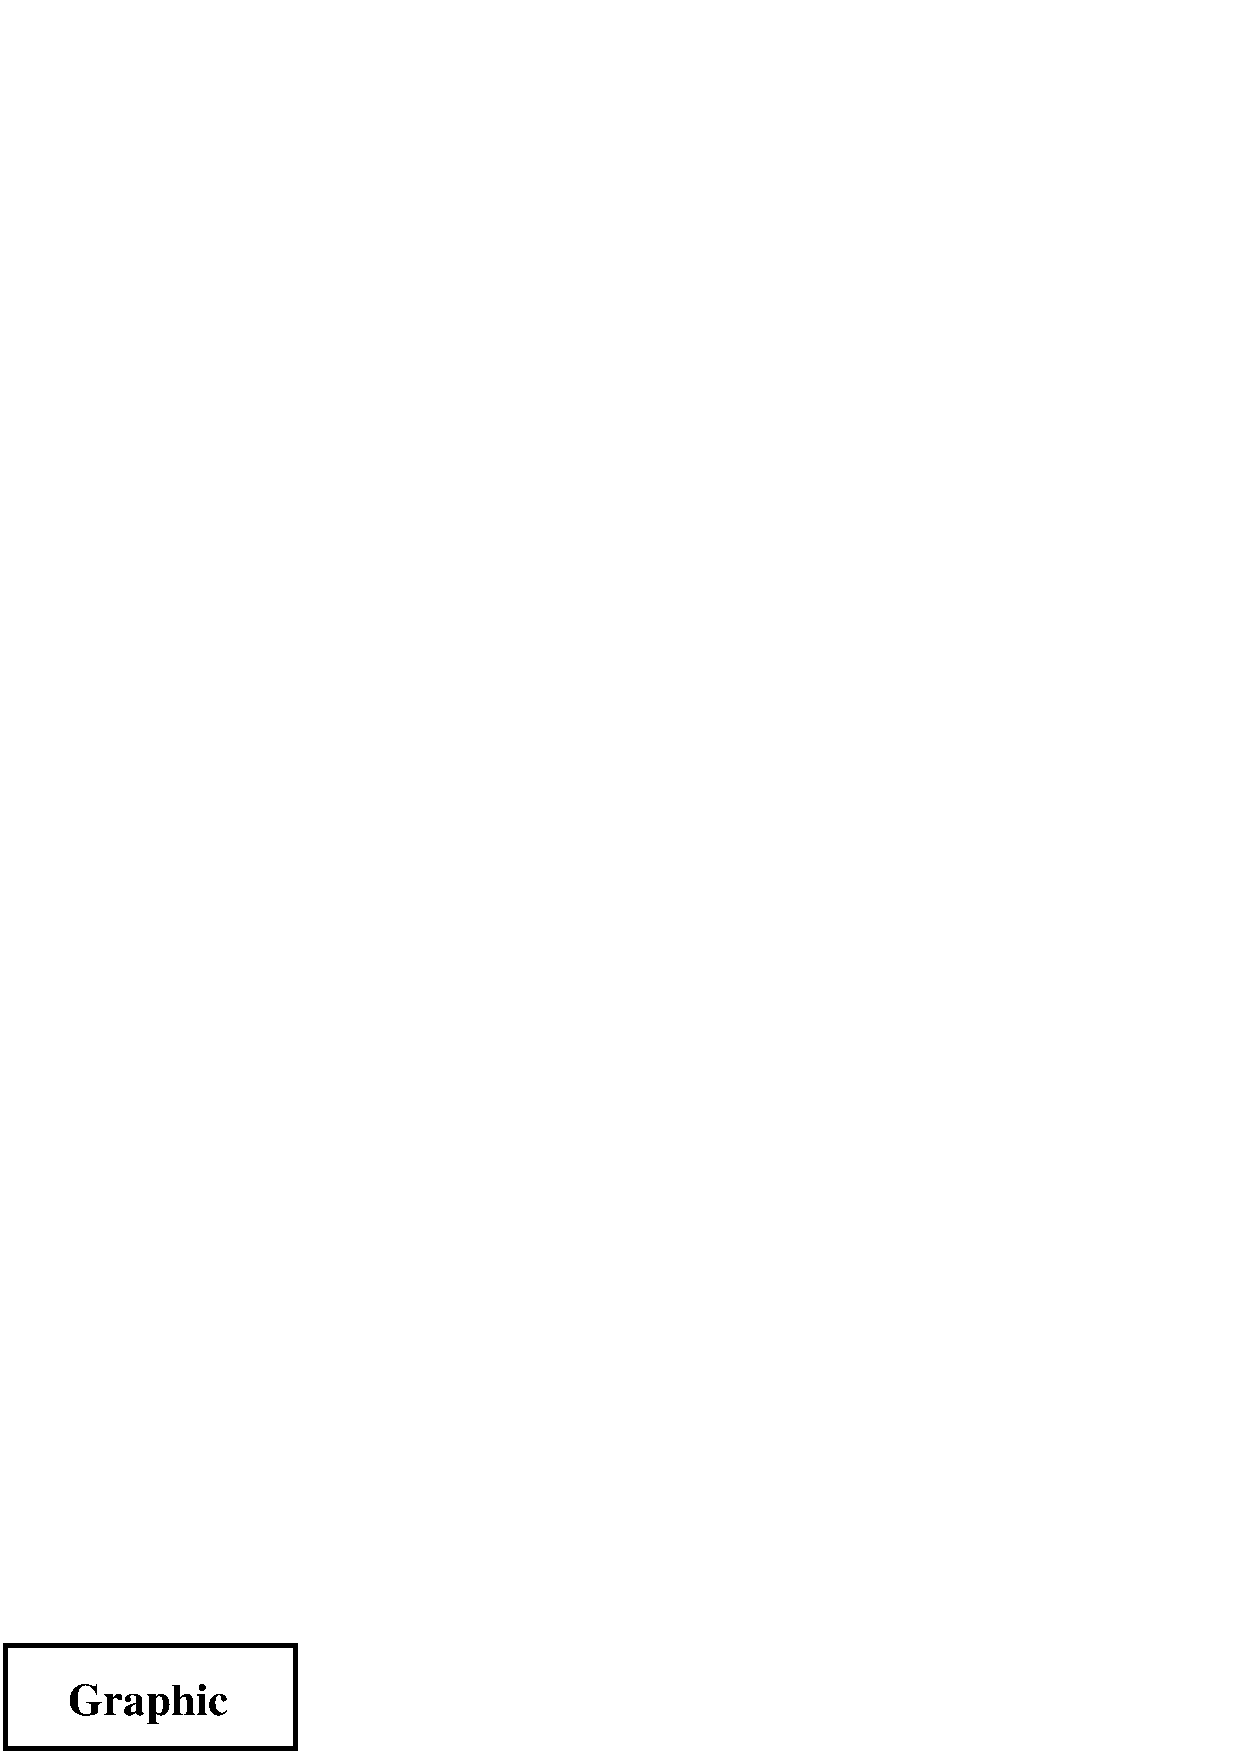
\includegraphics[width=1.0in]{graphic}}
	\hspace{1in}
	%%----start of second subfigure----
	\subfloat[Big Box]{
		\label{fig:subfig:b} %% label for second subfigure
		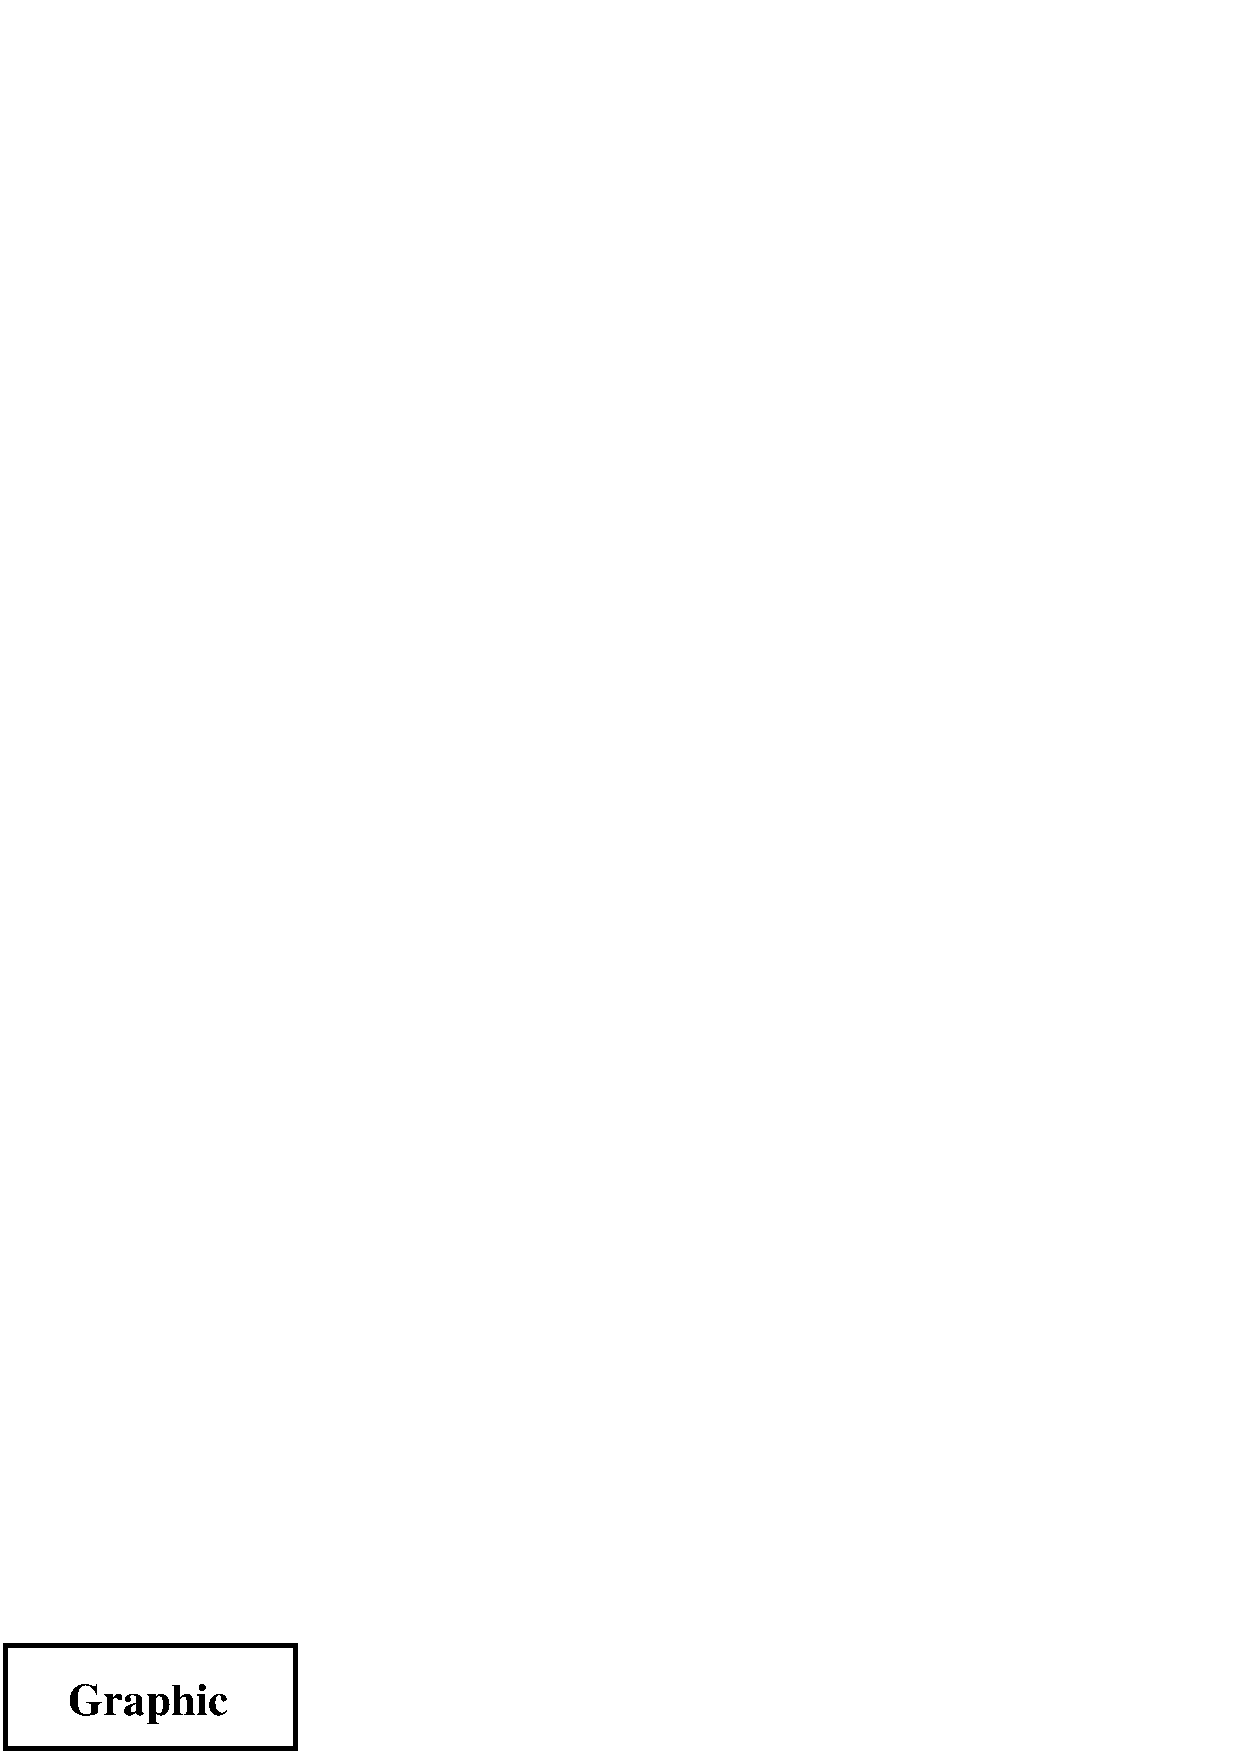
\includegraphics[width=1.5in]{graphic}}
	\caption{Two Subfigures}
	\label{fig:subfig} %% label for entire figure
\end{figure}

\begin{table}
	\centering
	\caption{图~\ref{fig:subfig} 的子图引用命令及其结果}
	\begin{tabular}{lc}
		\toprule
		引用命令 & 输出 \\
		\midrule
		\cmdM{subref}{fig:subfig:a} & \subref{fig:subfig:a} \\
		\cmdM{subref*}{fig:subfig:a} & \subref*{fig:subfig:a} \\
		\cmdM{ref}{fig:subfig:a} & \subref*{fig:subfig:a} \\
		\cmdM{subref}{fig:subfig:b} & \subref{fig:subfig:b} \\
		\cmdM{subref*}{fig:subfig:b} & \subref*{fig:subfig:b} \\
		\cmdM{ref}{fig:subfig:b} & \ref{fig:subfig:b} \\
		\cmdM{ref}{fig:subfig} & \ref{fig:subfig} \\
		\bottomrule
	\end{tabular}
\end{table}

\subsubsection{子图中的小页环境}

由于子图~\ref{fig:subfig:a} 只包含 \cmd{includegraphics} 命令,
因此子图~\ref{fig:subfig:a} 的标题宽度取决于插入图片的宽度。
如果子图中包含了小页环境,那么标题就可以和小页宽度一样了。
例如,
\begin{lstlisting}
\begin{figure}
	\subfloat[Small Box with a Long Caption]{
		\label{fig:mini:subfig:a} %% label for first subfigure
		\begin{minipage}[b]{0.45\linewidth}
			\centering 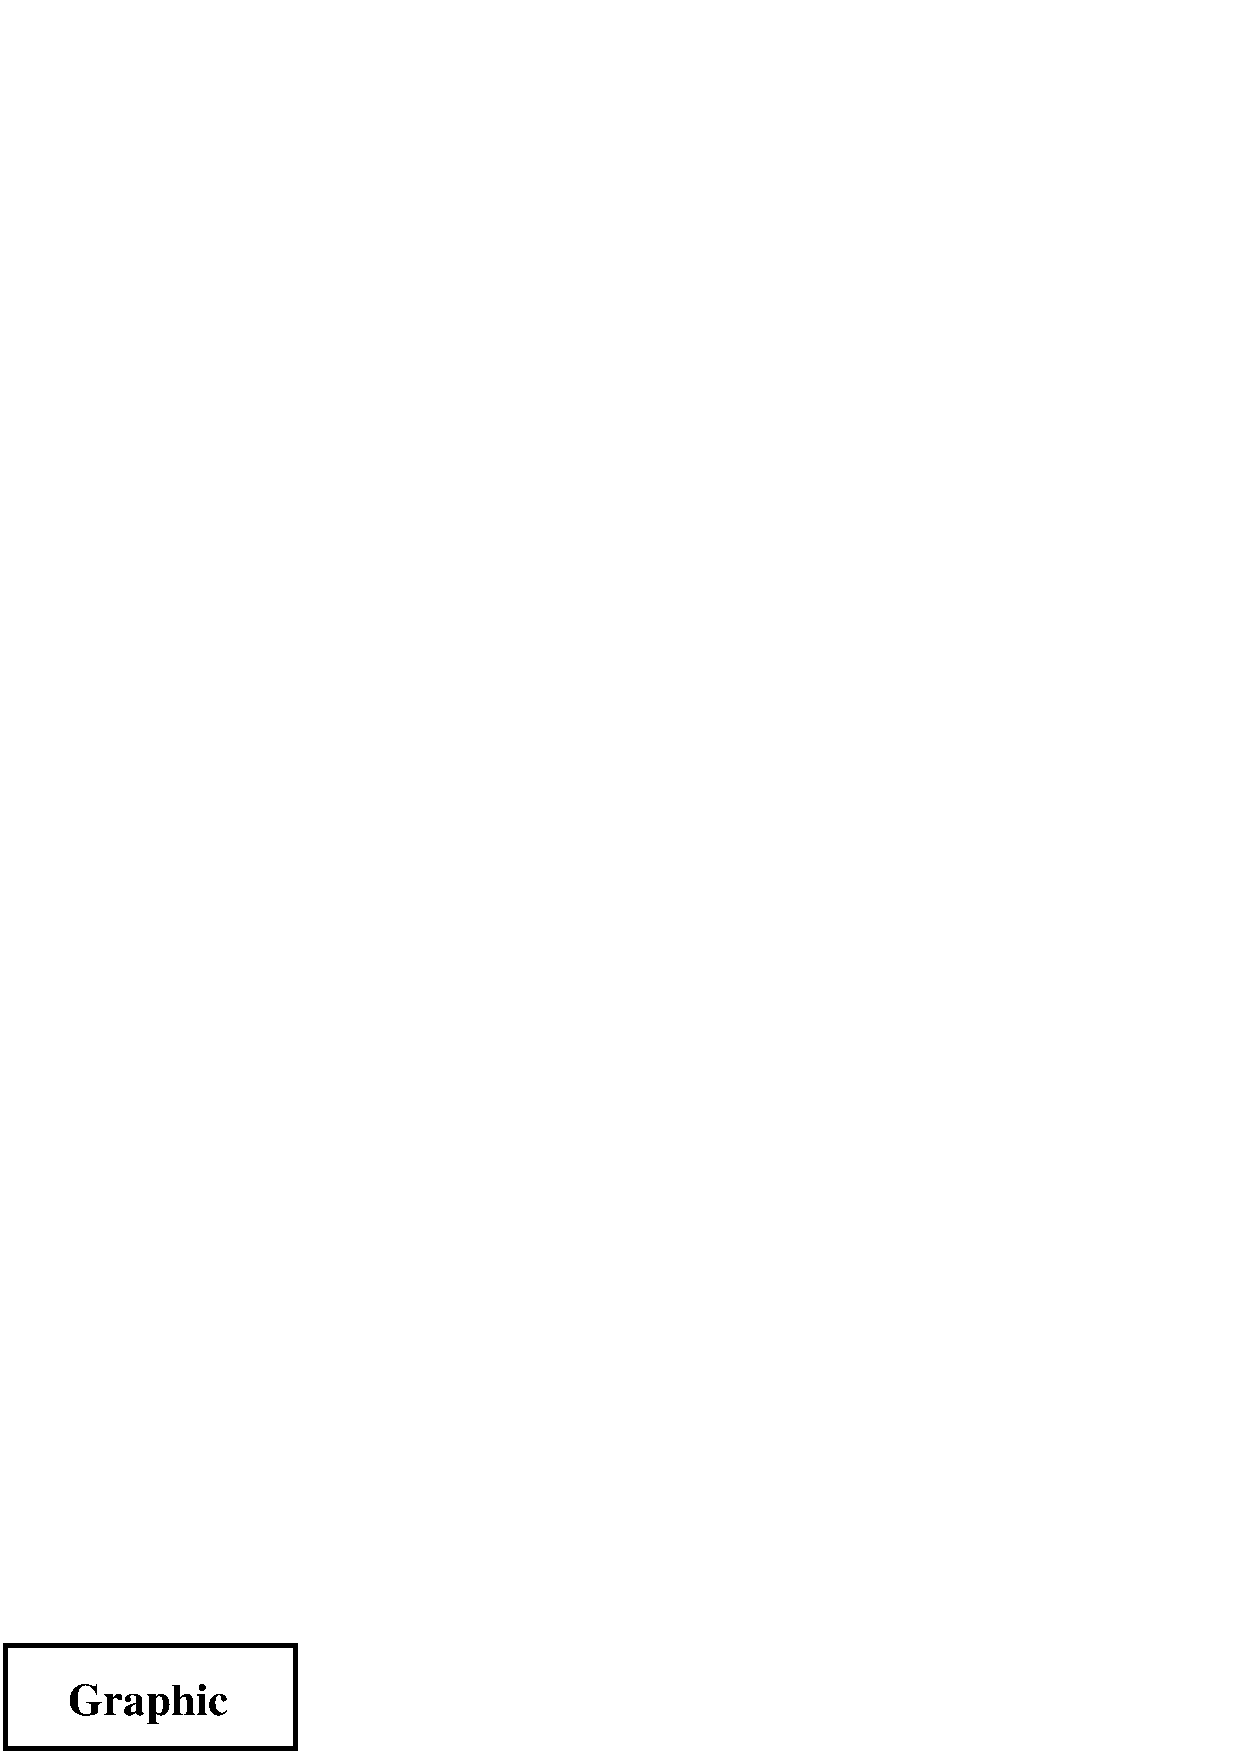
\includegraphics[width=1in]{graphic}
		\end{minipage}}%
	\hfill
	\subfloat[Big Box]{
		\label{fig:mini:subfig:b} %% label for second subfigure
		\begin{minipage}[b]{0.45\linewidth}
			\centering 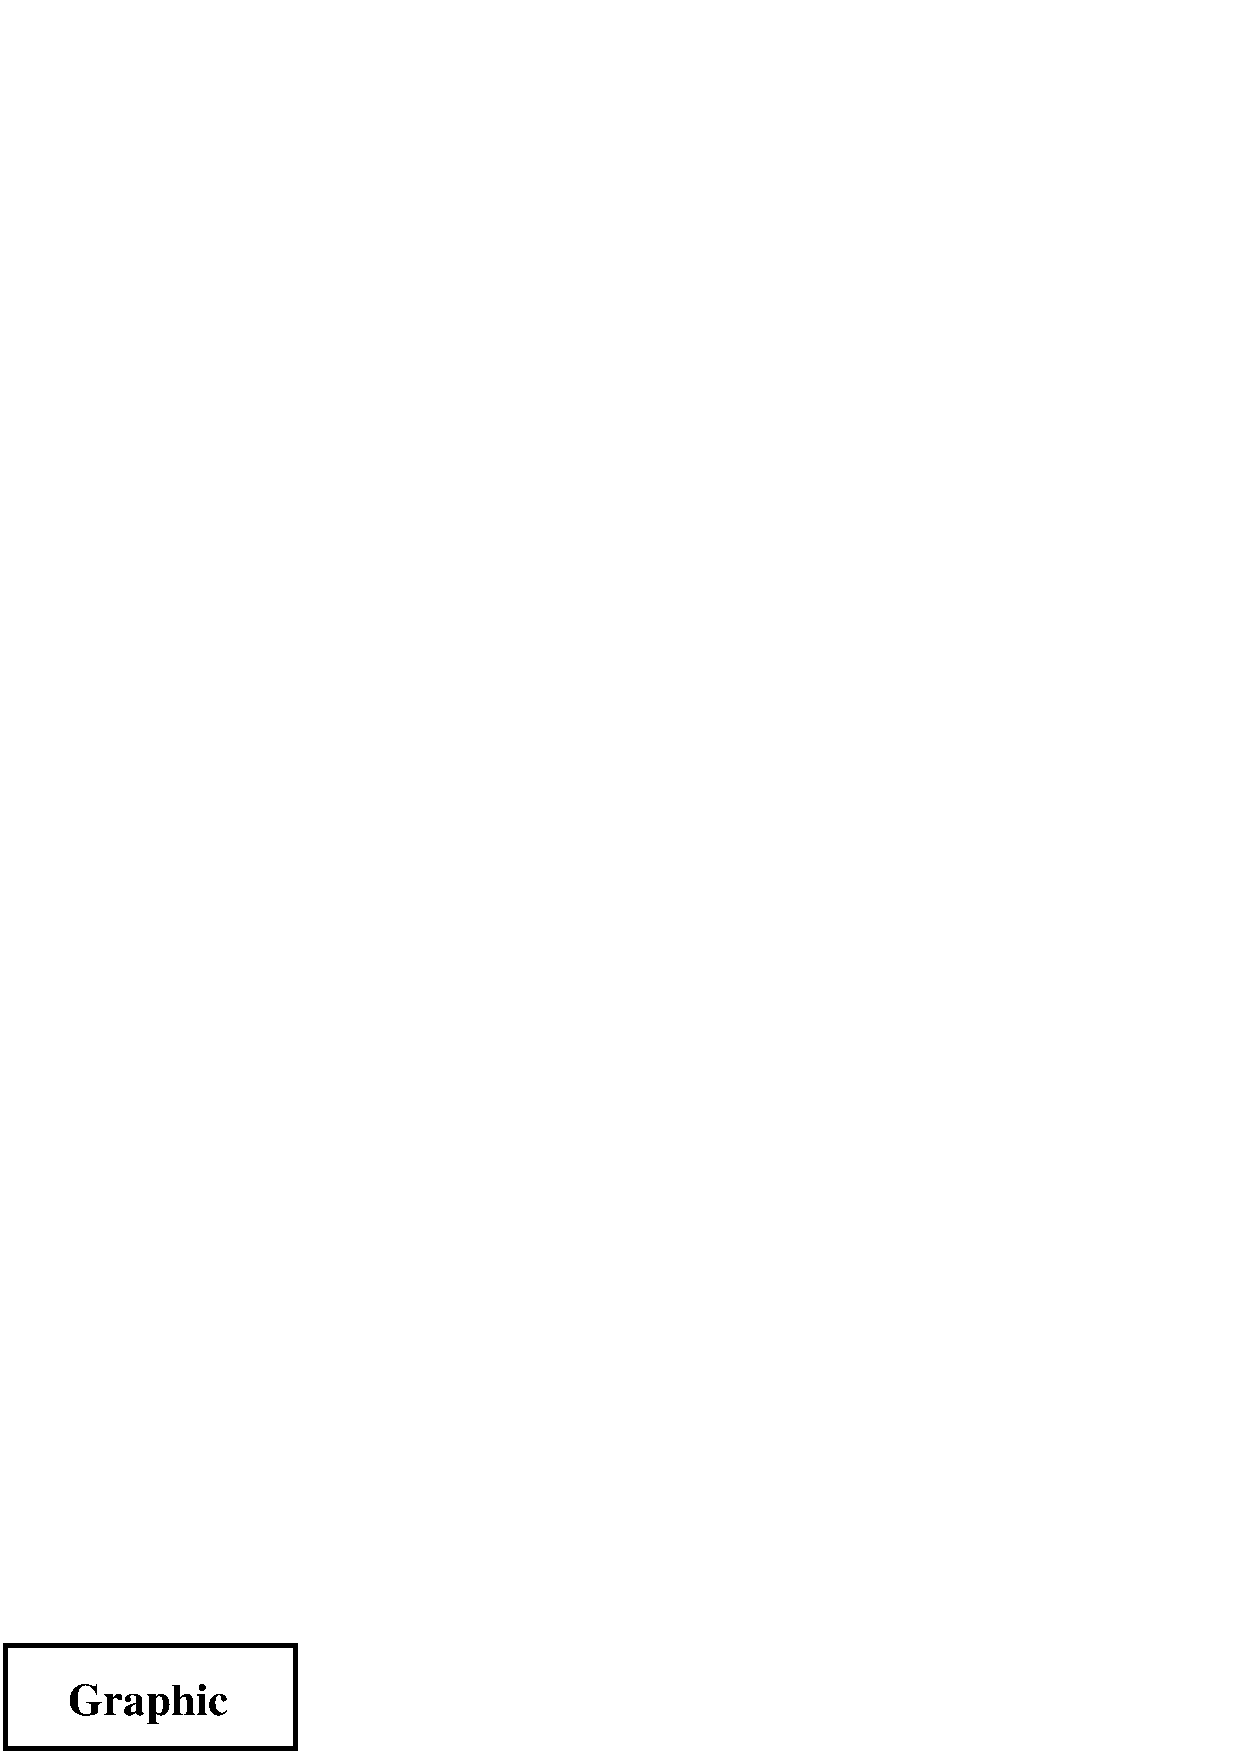
\includegraphics[width=1.5in]{graphic}
		\end{minipage}}
	\caption{Minipages Inside Subfigures}
	\label{fig:mini:subfig} %% label for entire figure
\end{figure}
\end{lstlisting}
生成图~\ref{fig:mini:subfig},其中包含了子图~\ref{fig:mini:subfig:a} 和~\ref{fig:mini:subfig:b}。

\begin{figure}
	\subfloat[Small Box with a Long Caption]{
		\label{fig:mini:subfig:a} %% label for first subfigure
		\begin{minipage}[b]{0.45\linewidth}
			\centering 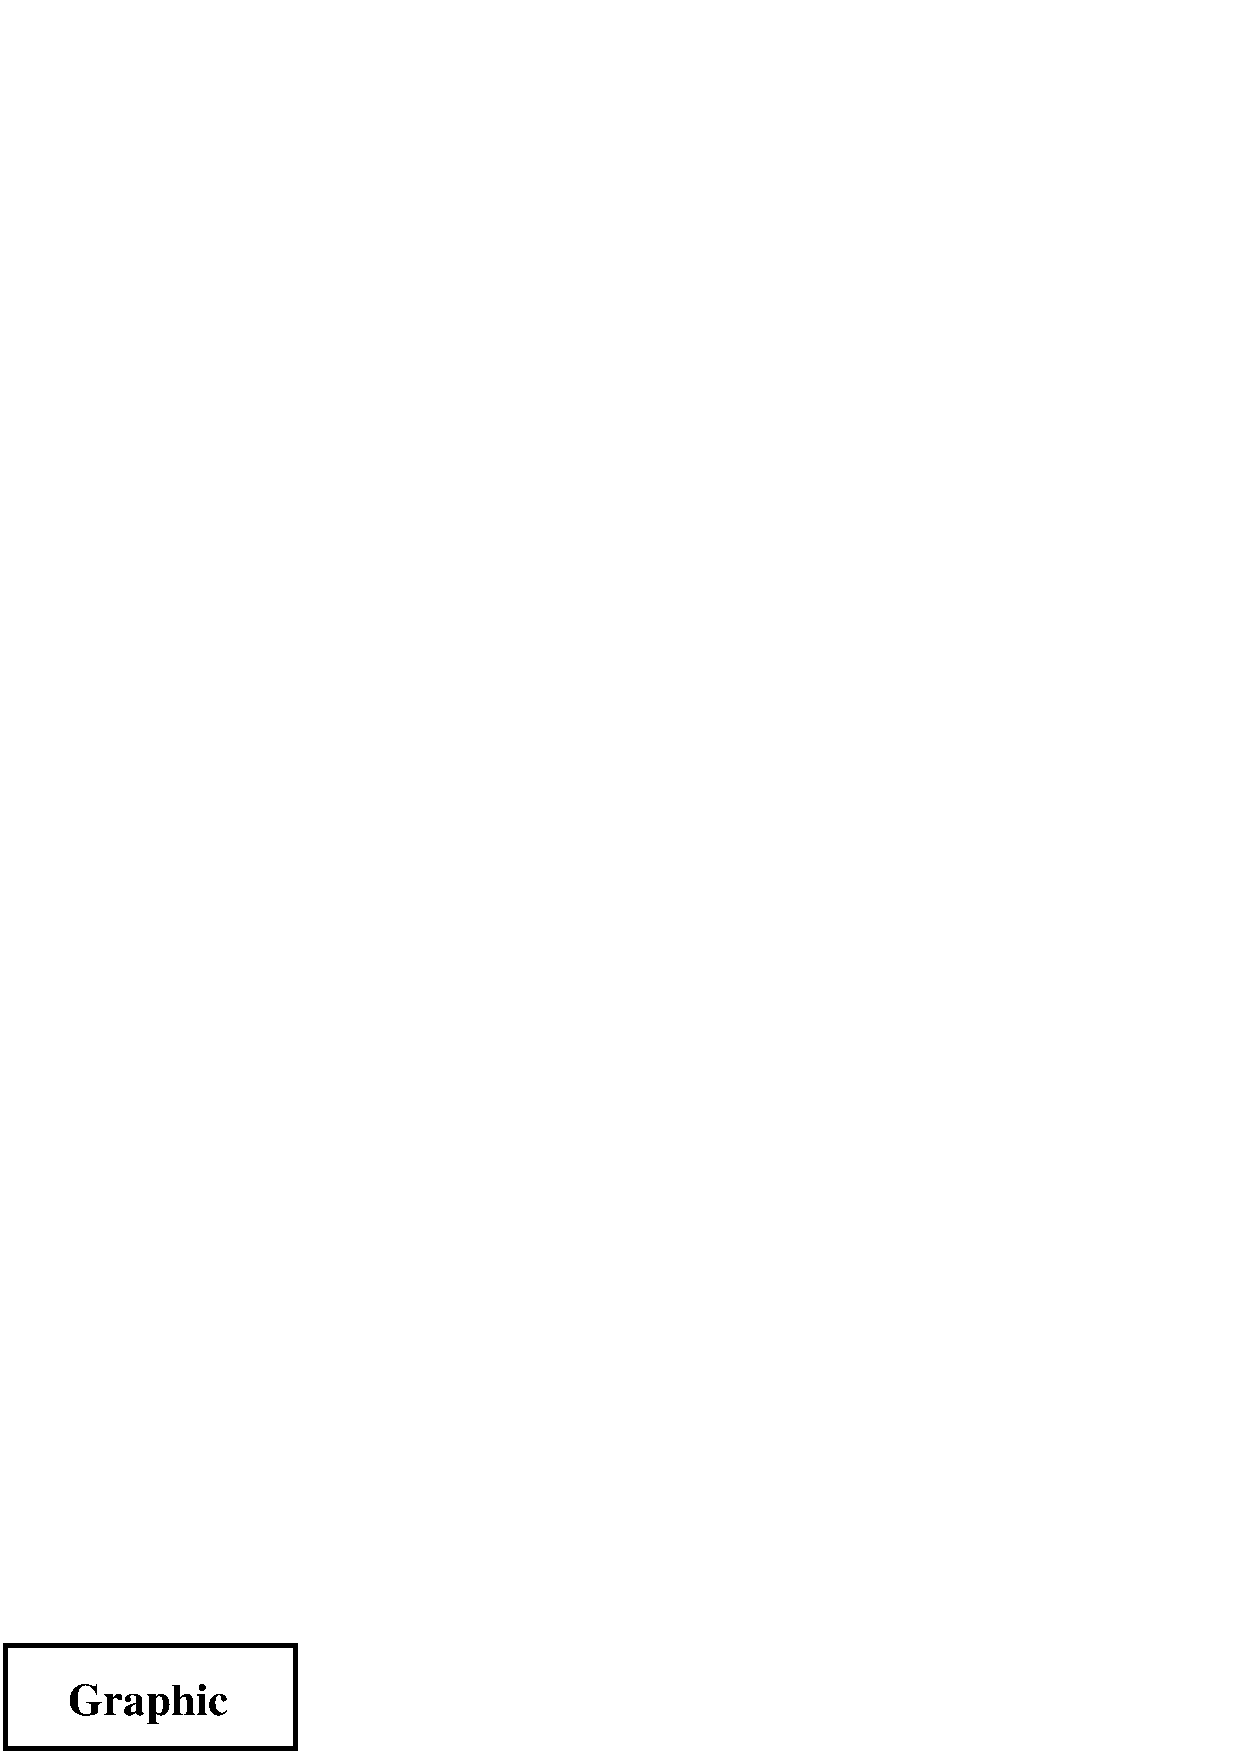
\includegraphics[width=1in]{graphic}
		\end{minipage}}%
		\hfill
		\subfloat[Big Box]{
			\label{fig:mini:subfig:b} %% label for second subfigure
			\begin{minipage}[b]{0.45\linewidth}
				\centering 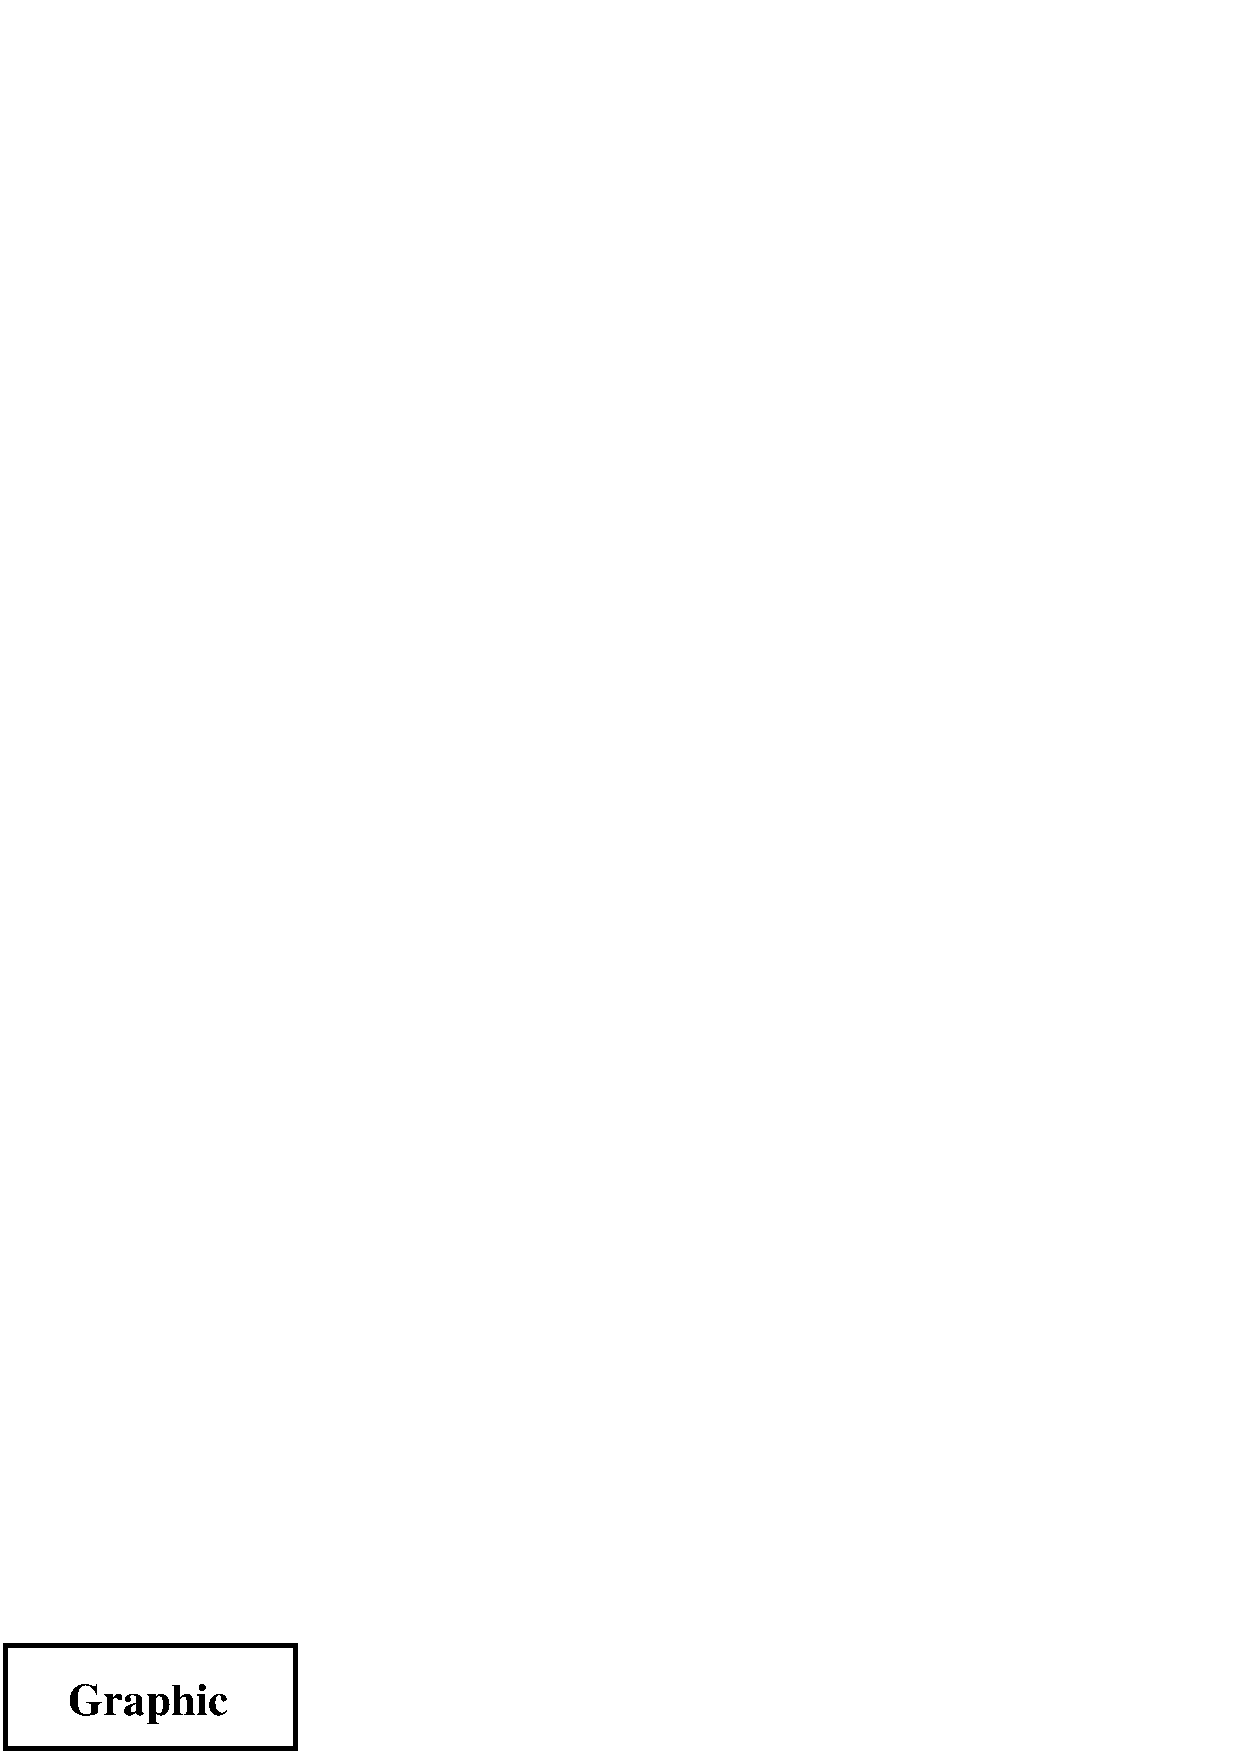
\includegraphics[width=1.5in]{graphic}
			\end{minipage}}
			\caption{Minipages Inside Subfigures}
			\label{fig:mini:subfig} %% label for entire figure
		\end{figure}

由于子图标题的宽度默认就是子图的宽度,
因此图~\ref{fig:mini:subfig} 中子图标题的宽度大于图~\ref{fig:subfig} 中的子图标题。
这是因为图~\ref{fig:subfig} 中的子图只包含图像,
而图~\ref{fig:mini:subfig} 中的子图包含了宽度为 $0.5\text{\cmd{linewidth}}$ 的小页环境。


\section{标题中分开的小页环境}

第~\ref{ssec:sidefigure} 节描述了如何通过在小页环境中同时使用插图命令和 \cmd{caption} 命令来构建并列图形。
本节将介绍如何通过在不同的小页环境中使用插图命令和 \cmd{caption} 命令来获得更好的对齐效果。

在图~\ref{fig:side:a}~和~\ref{fig:side:b}中,
并列的小页环境使用了 \opt{[t]}~选项,进而使得两幅图形的基线对齐。
这对于非旋转的图形没有任何问题,而且使得两标题的顶部对齐。
不过,如果图形的底部不对齐的话(如其中一图形被旋转),就会发生问题。例如:
\begin{lstlisting}
\begin{figure}
	\centering
	%%----start of first figure----
	\begin{minipage}[t]{.4\linewidth}
		\centering
		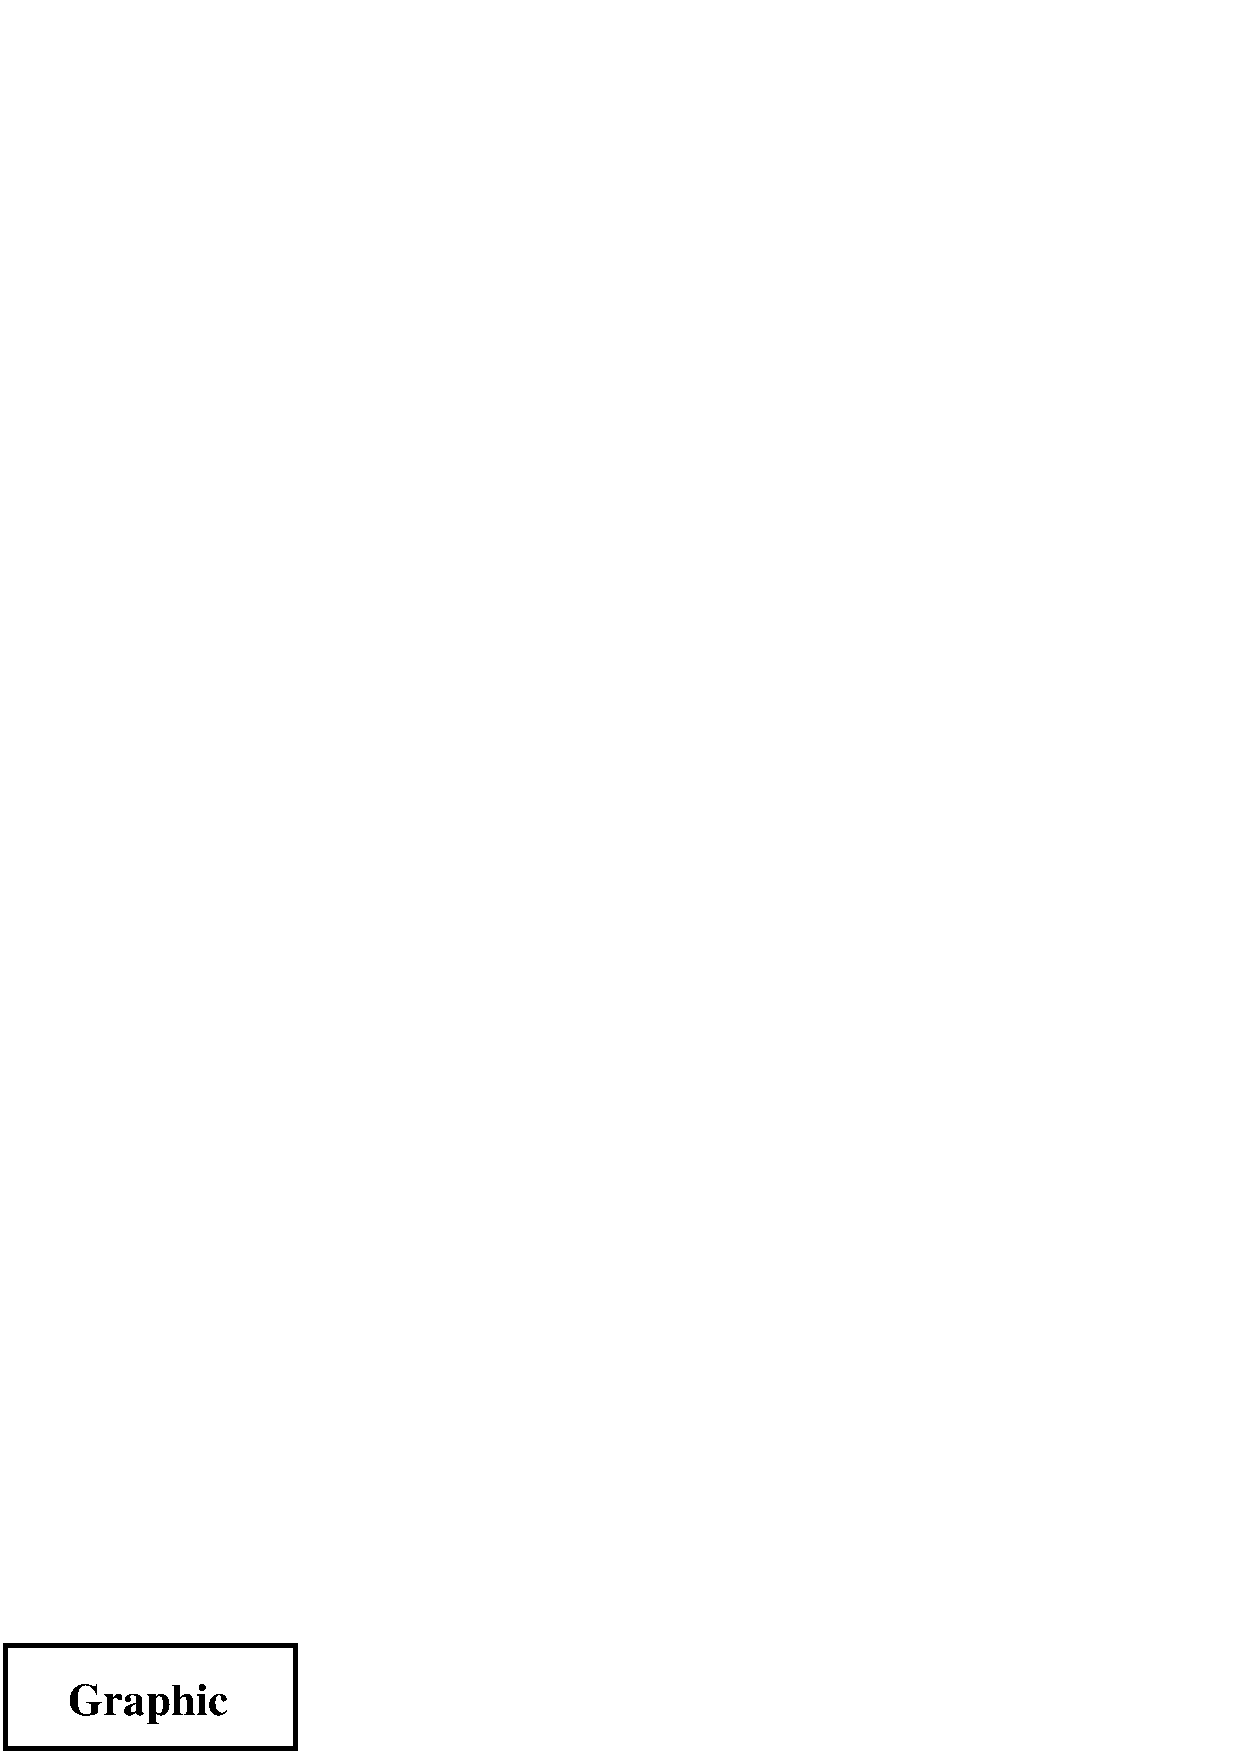
\includegraphics[width=2cm]{graphic}
		\caption{Box with a Long Caption}
	\end{minipage}%
	\hspace{1cm}%
	%%----start of second figure----
	\begin{minipage}[t]{.4\linewidth}
		\centering
		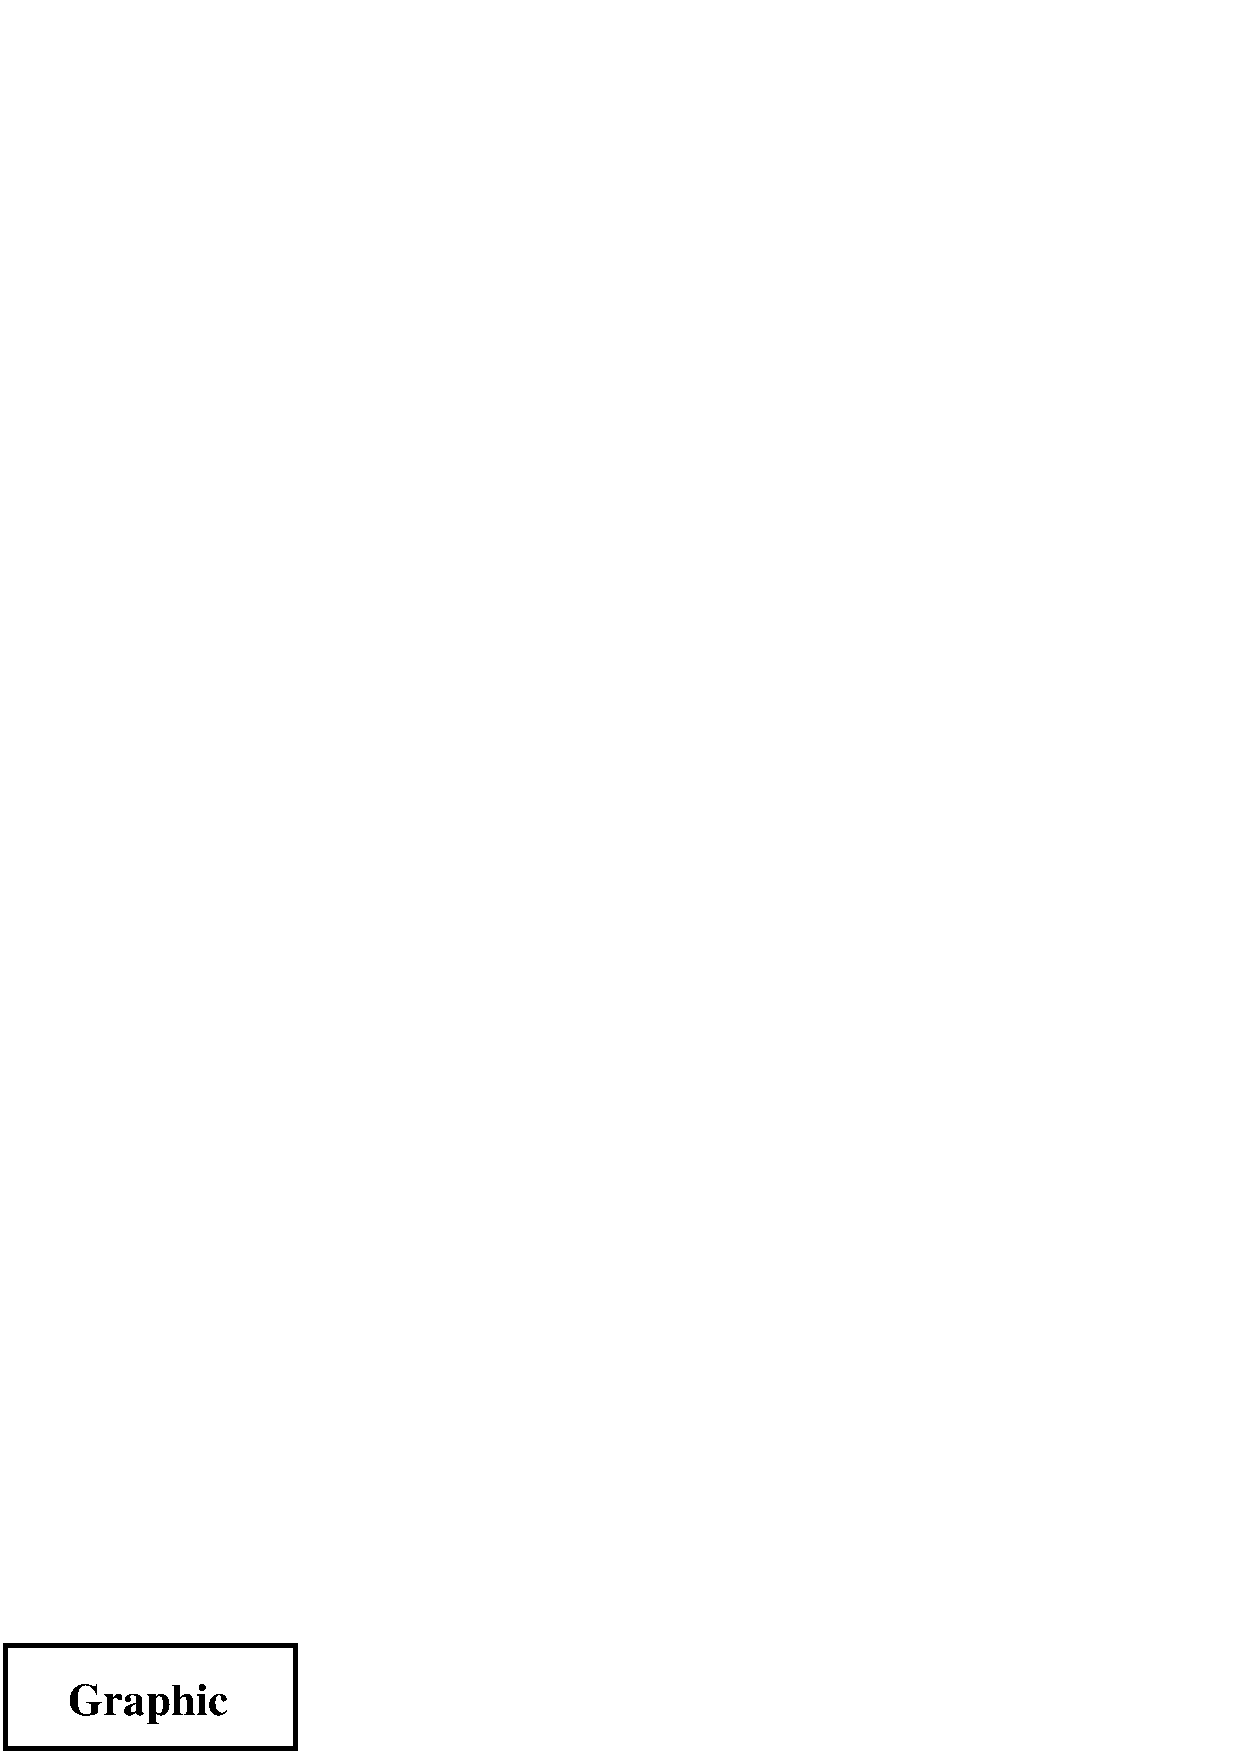
\includegraphics[width=2cm,angle=-30]{graphic}
		\caption{Rotated Box}
	\end{minipage}%
\end{figure}
\end{lstlisting}
生成图~\ref{fig:mininonrot}~和~\ref{fig:minirot},
我们可以看到这里两幅图形的标题并不对齐。
而若只使用小页的 \opt{[b]} 选项,会使得标题的最后一行对齐,并不能解决问题。

\begin{figure}
	\centering
	%%----start of first figure----
	\begin{minipage}[t]{.4\linewidth}
		\centering
		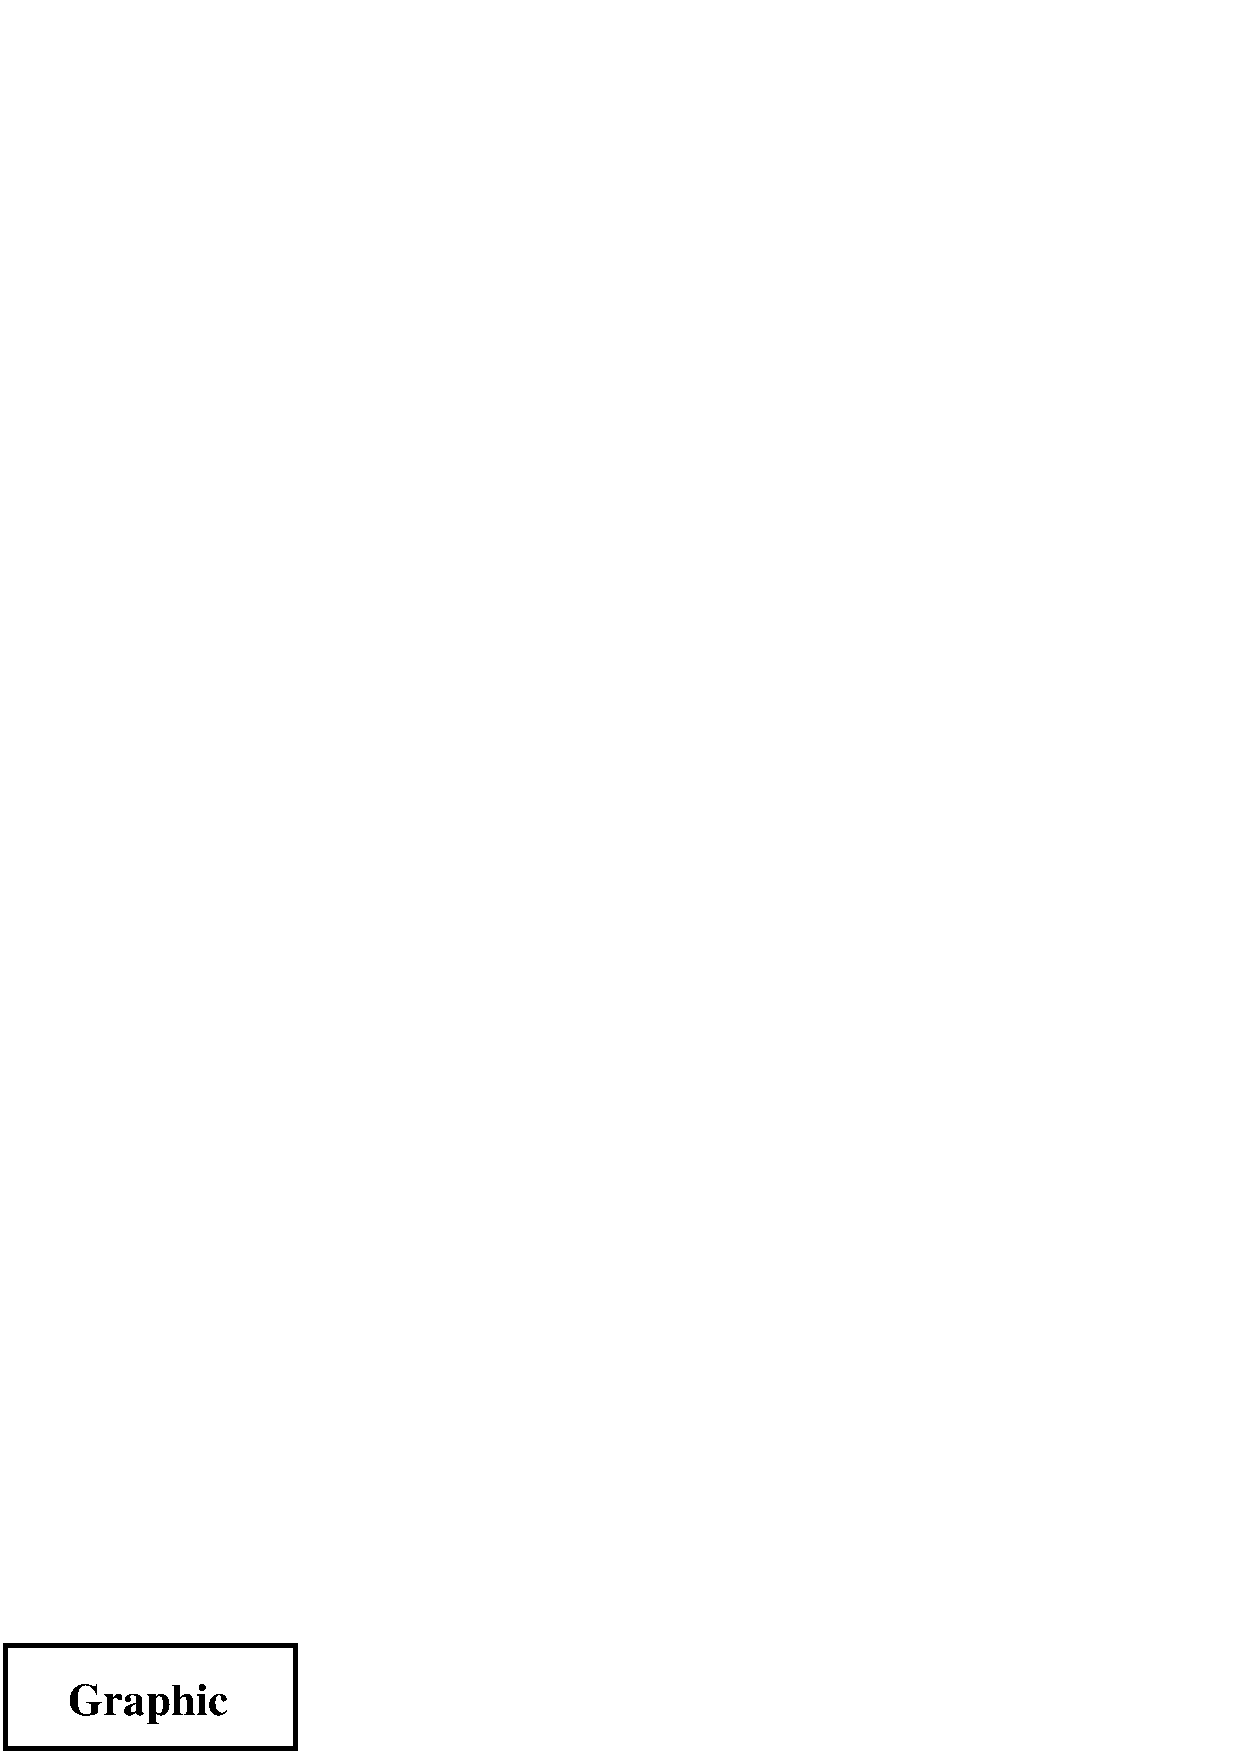
\includegraphics[width=2cm]{graphic}
		\caption{Box with a Long Caption}\label{fig:mininonrot} 
	\end{minipage}%
	\hspace{1cm}%
	%%----start of second figure----
	\begin{minipage}[t]{.4\linewidth}
		\centering
		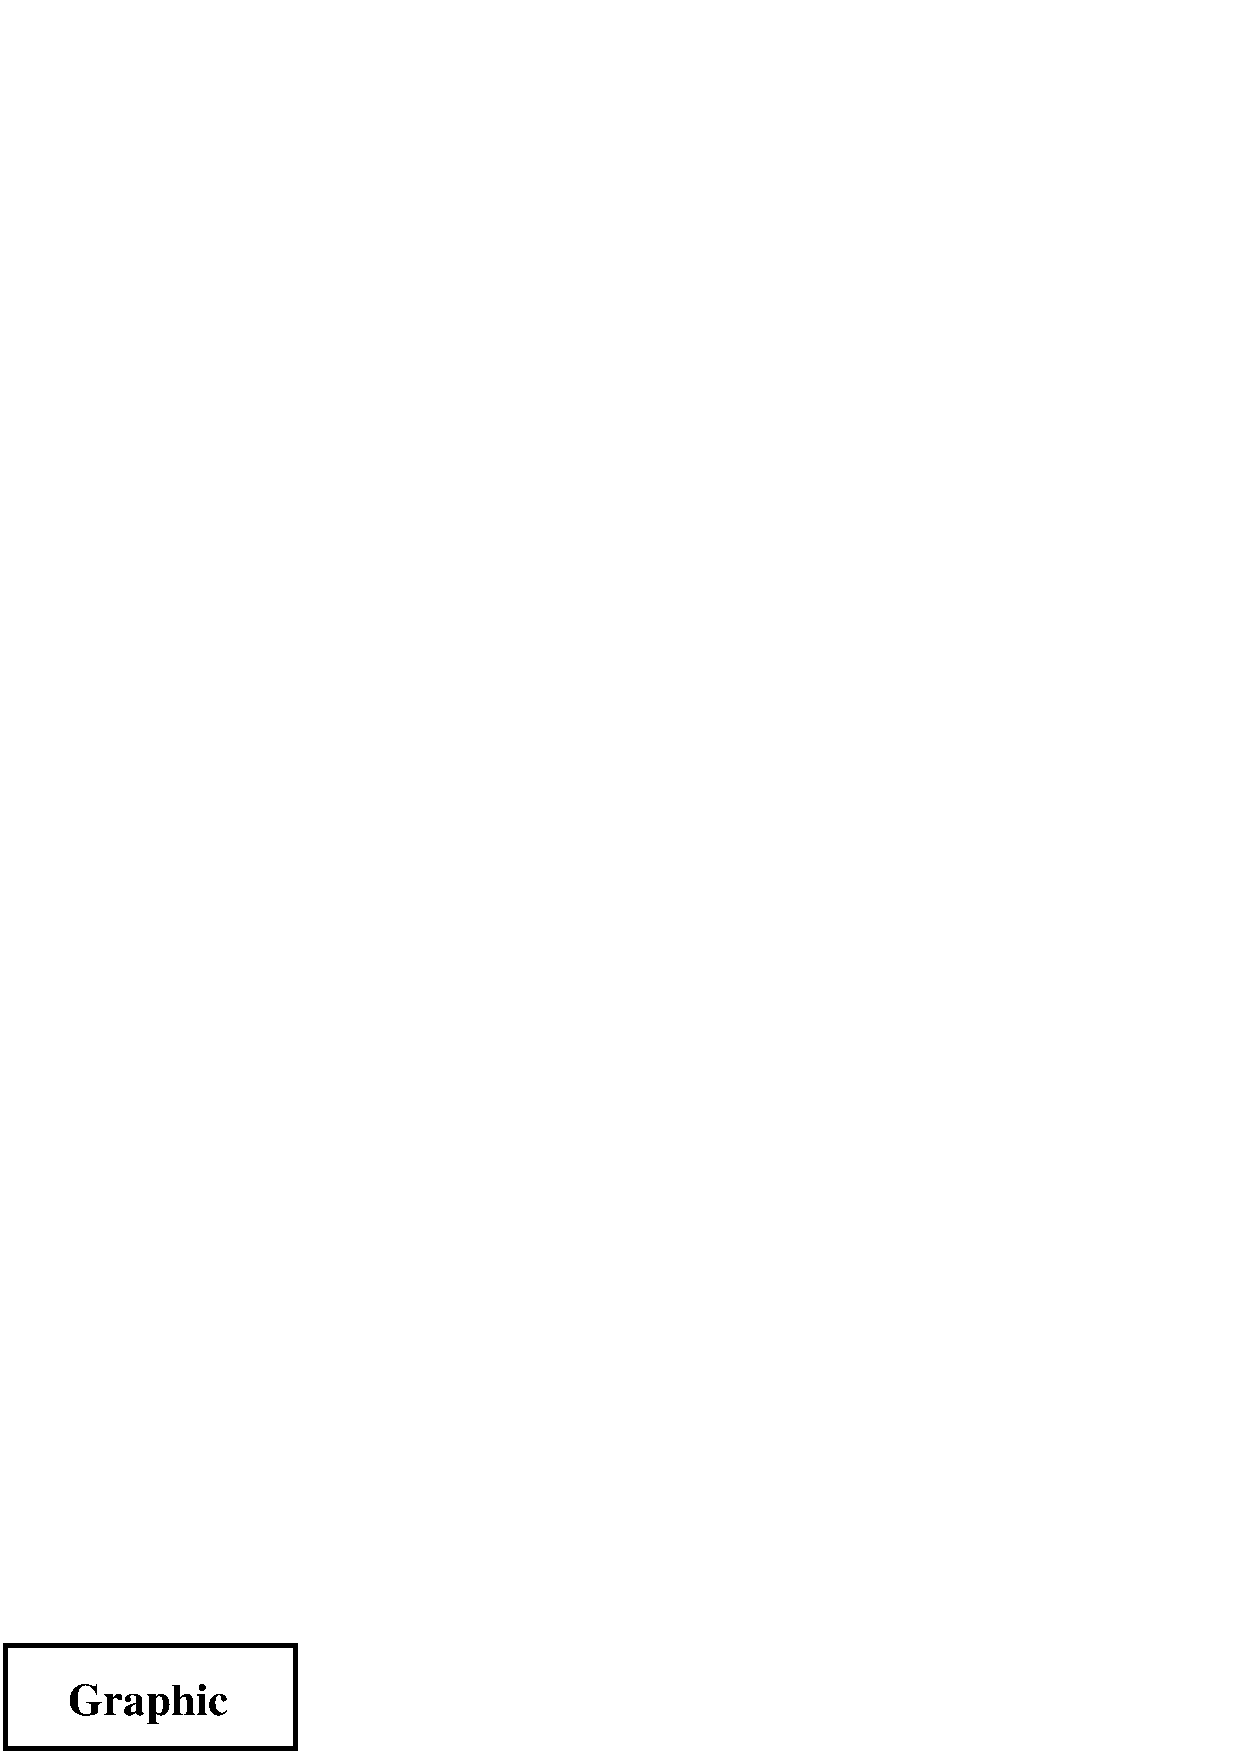
\includegraphics[width=2cm,angle=-30]{graphic}
		\caption{Rotated Box}\label{fig:minirot} 
	\end{minipage}%
\end{figure}

一种解决办法是在创建两行小页环境,并把图形和标题分开放置:
第一行放置图形,第二行放置标题。例如:
\begin{lstlisting}
\begin{figure}
	\centering
	%%----start of first figure graphics----
	\begin{minipage}[b]{.4\linewidth}
		\centering
		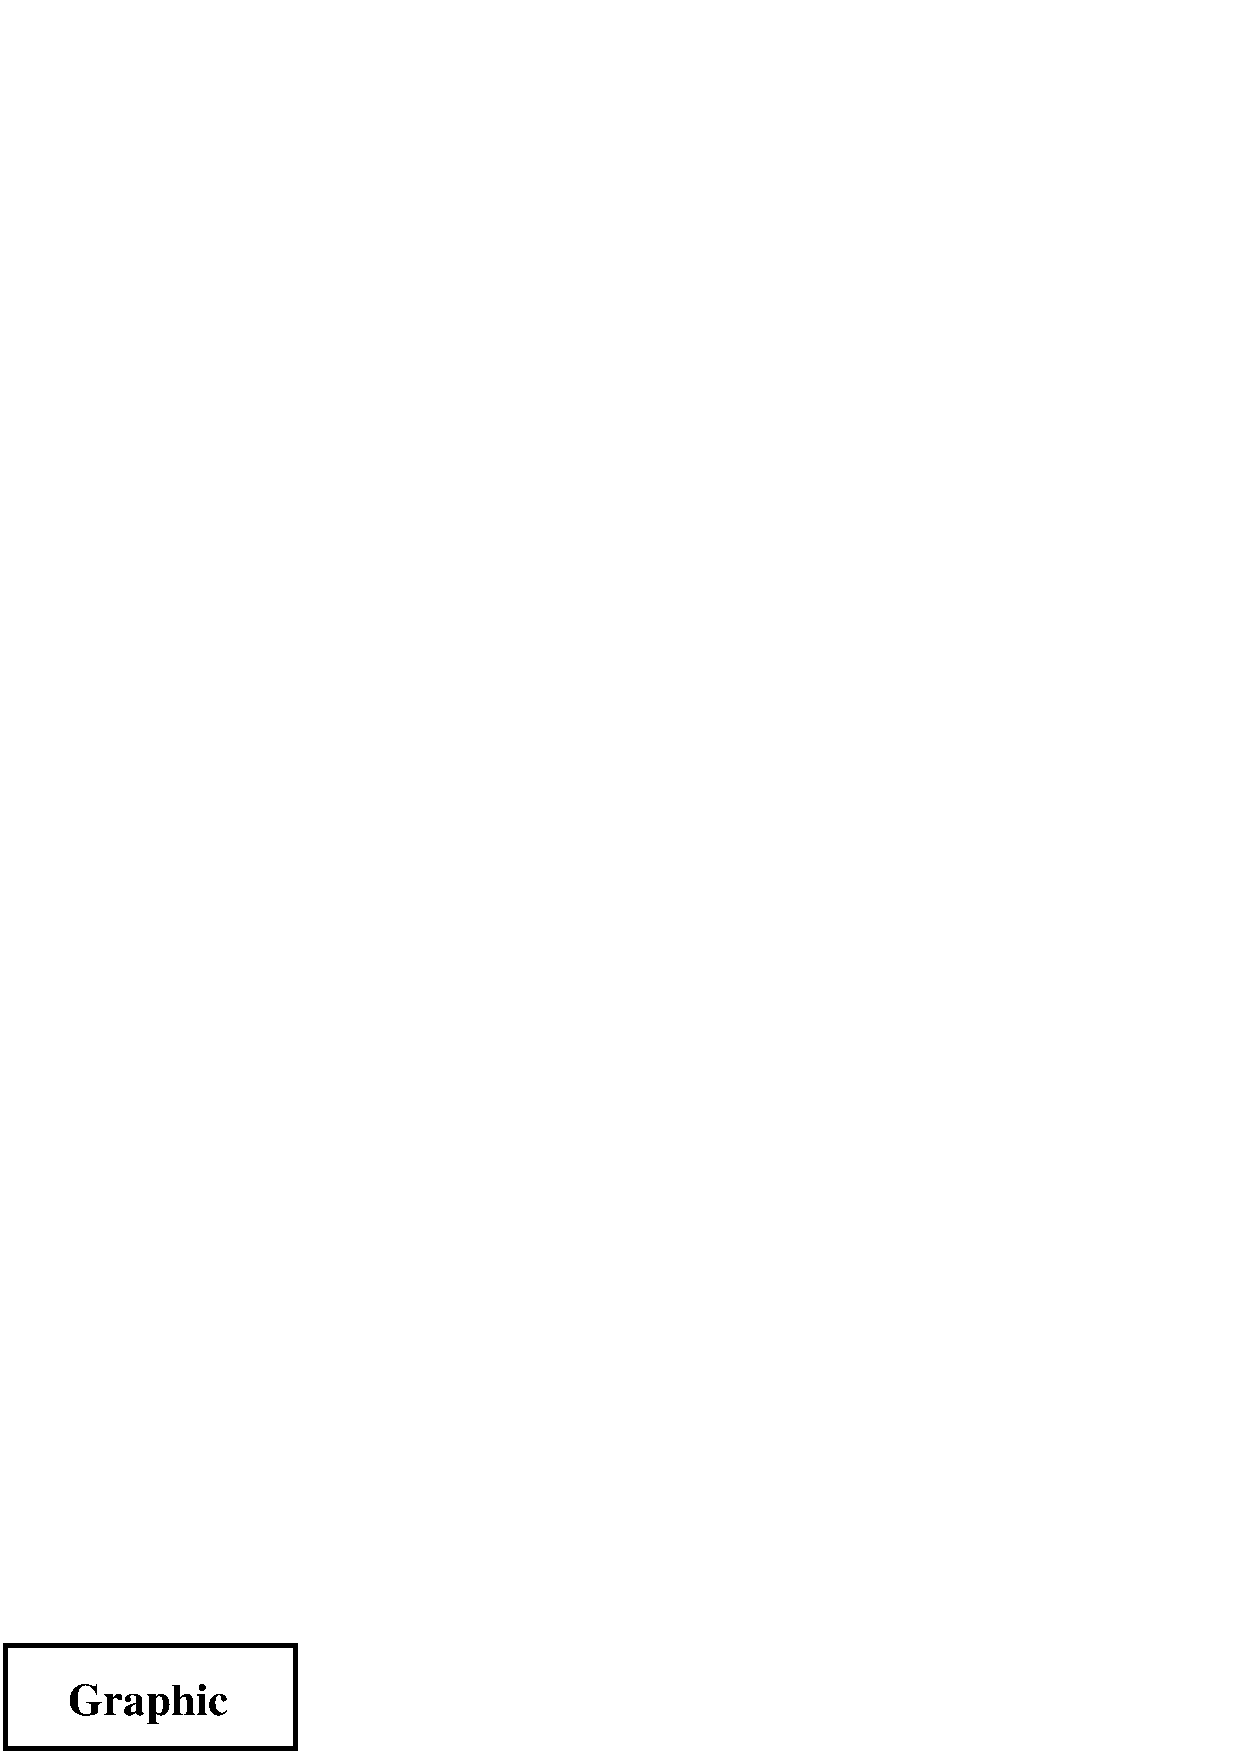
\includegraphics[width=2cm]{graphic}
	\end{minipage}%
	\hspace{1cm}%
	%%----start of second figure graphics----
	\begin{minipage}[b]{.4\linewidth}
		\centering
		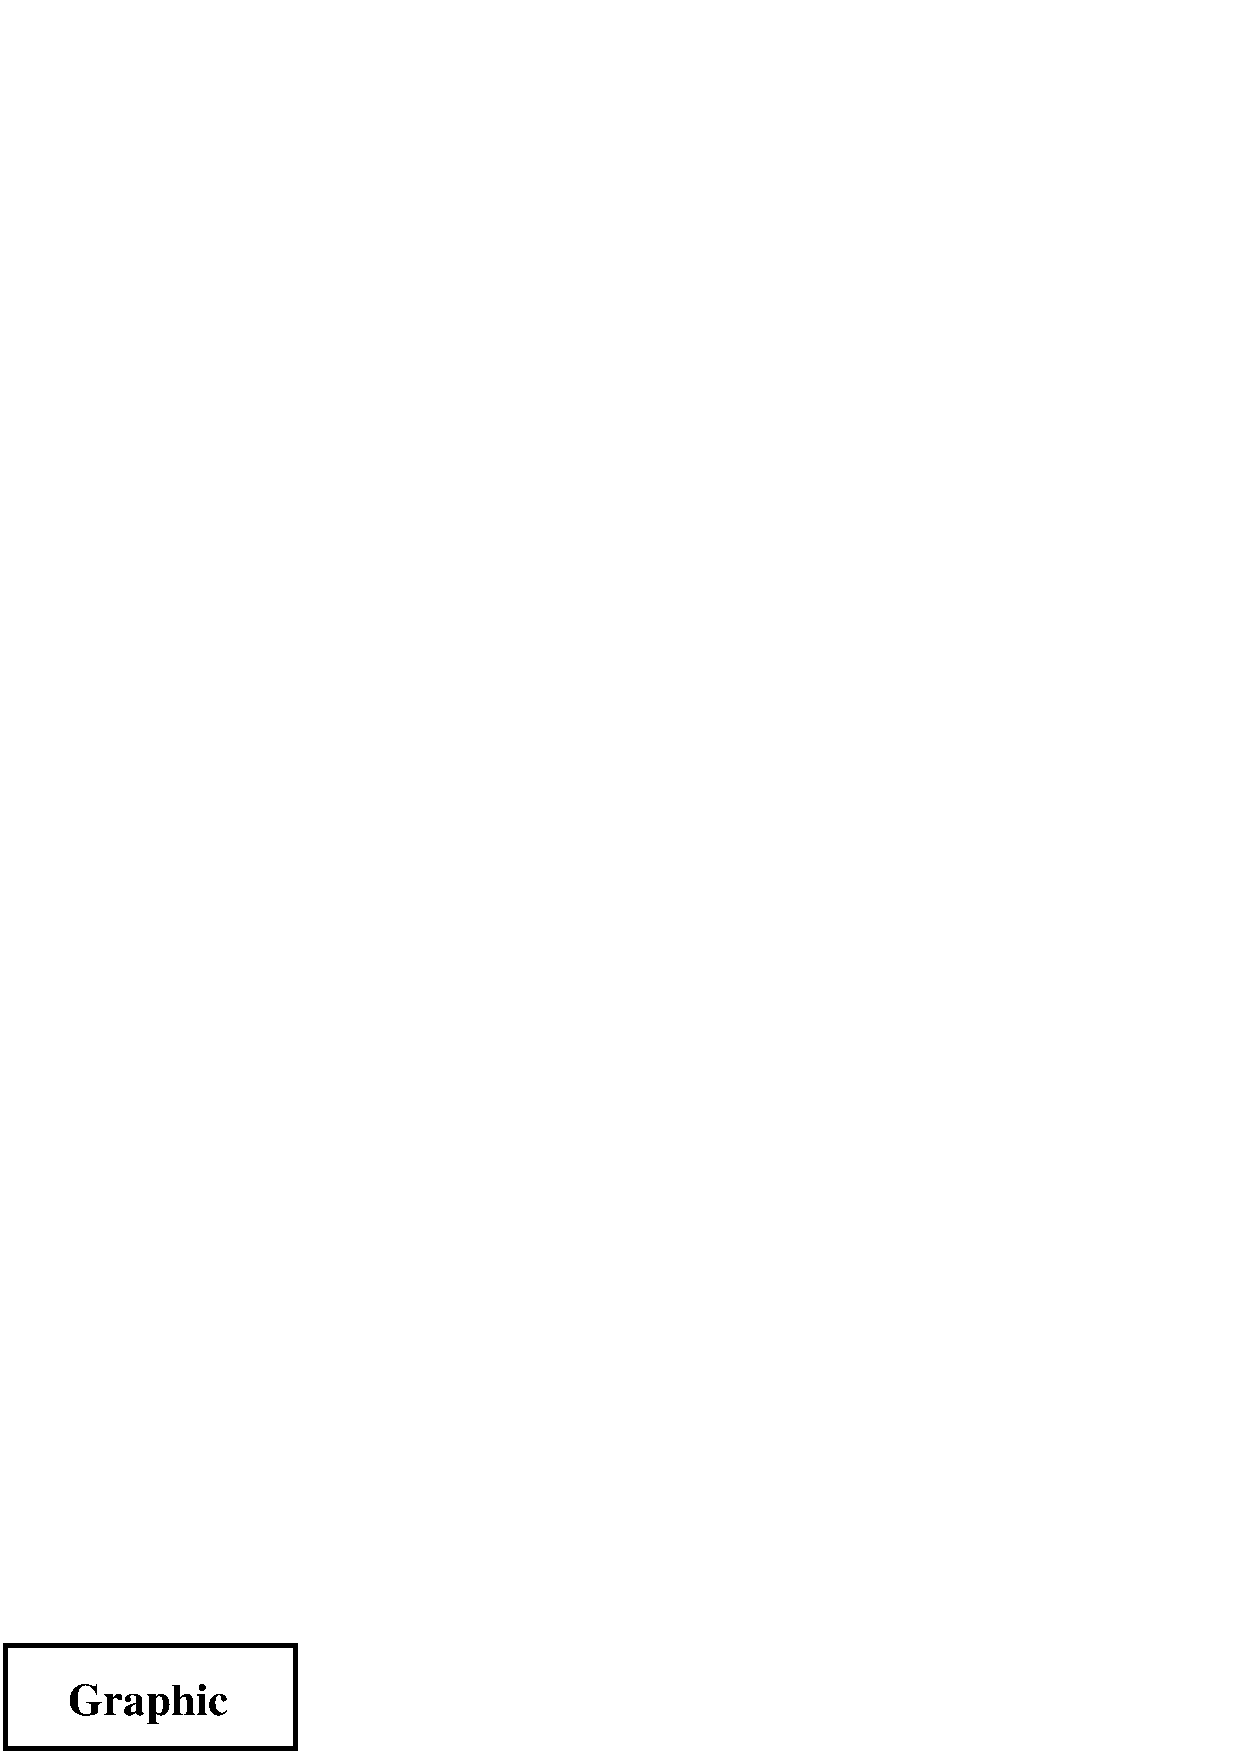
\includegraphics[width=2cm,angle=-30]{graphic}
	\end{minipage}\\[-10pt]
	%%----start of first figure caption----
	\begin{minipage}[t]{.4\linewidth}
		\caption{Box with a Long Caption}
	\end{minipage}%
	\hspace{1cm}%
	%%----start of second figure caption----
	\begin{minipage}[t]{.4\linewidth}
		\caption{Rotated Box}
	\end{minipage}%
\end{figure}
\end{lstlisting}
生成的图~\ref{fig:mininonrot:a}~和~\ref{fig:minirot:a}~中,
图形的基线和标题的第一行分别对齐。

\begin{figure}
	\centering
	%%----start of first figure graphics----
	\begin{minipage}[b]{.4\linewidth}
		\centering
		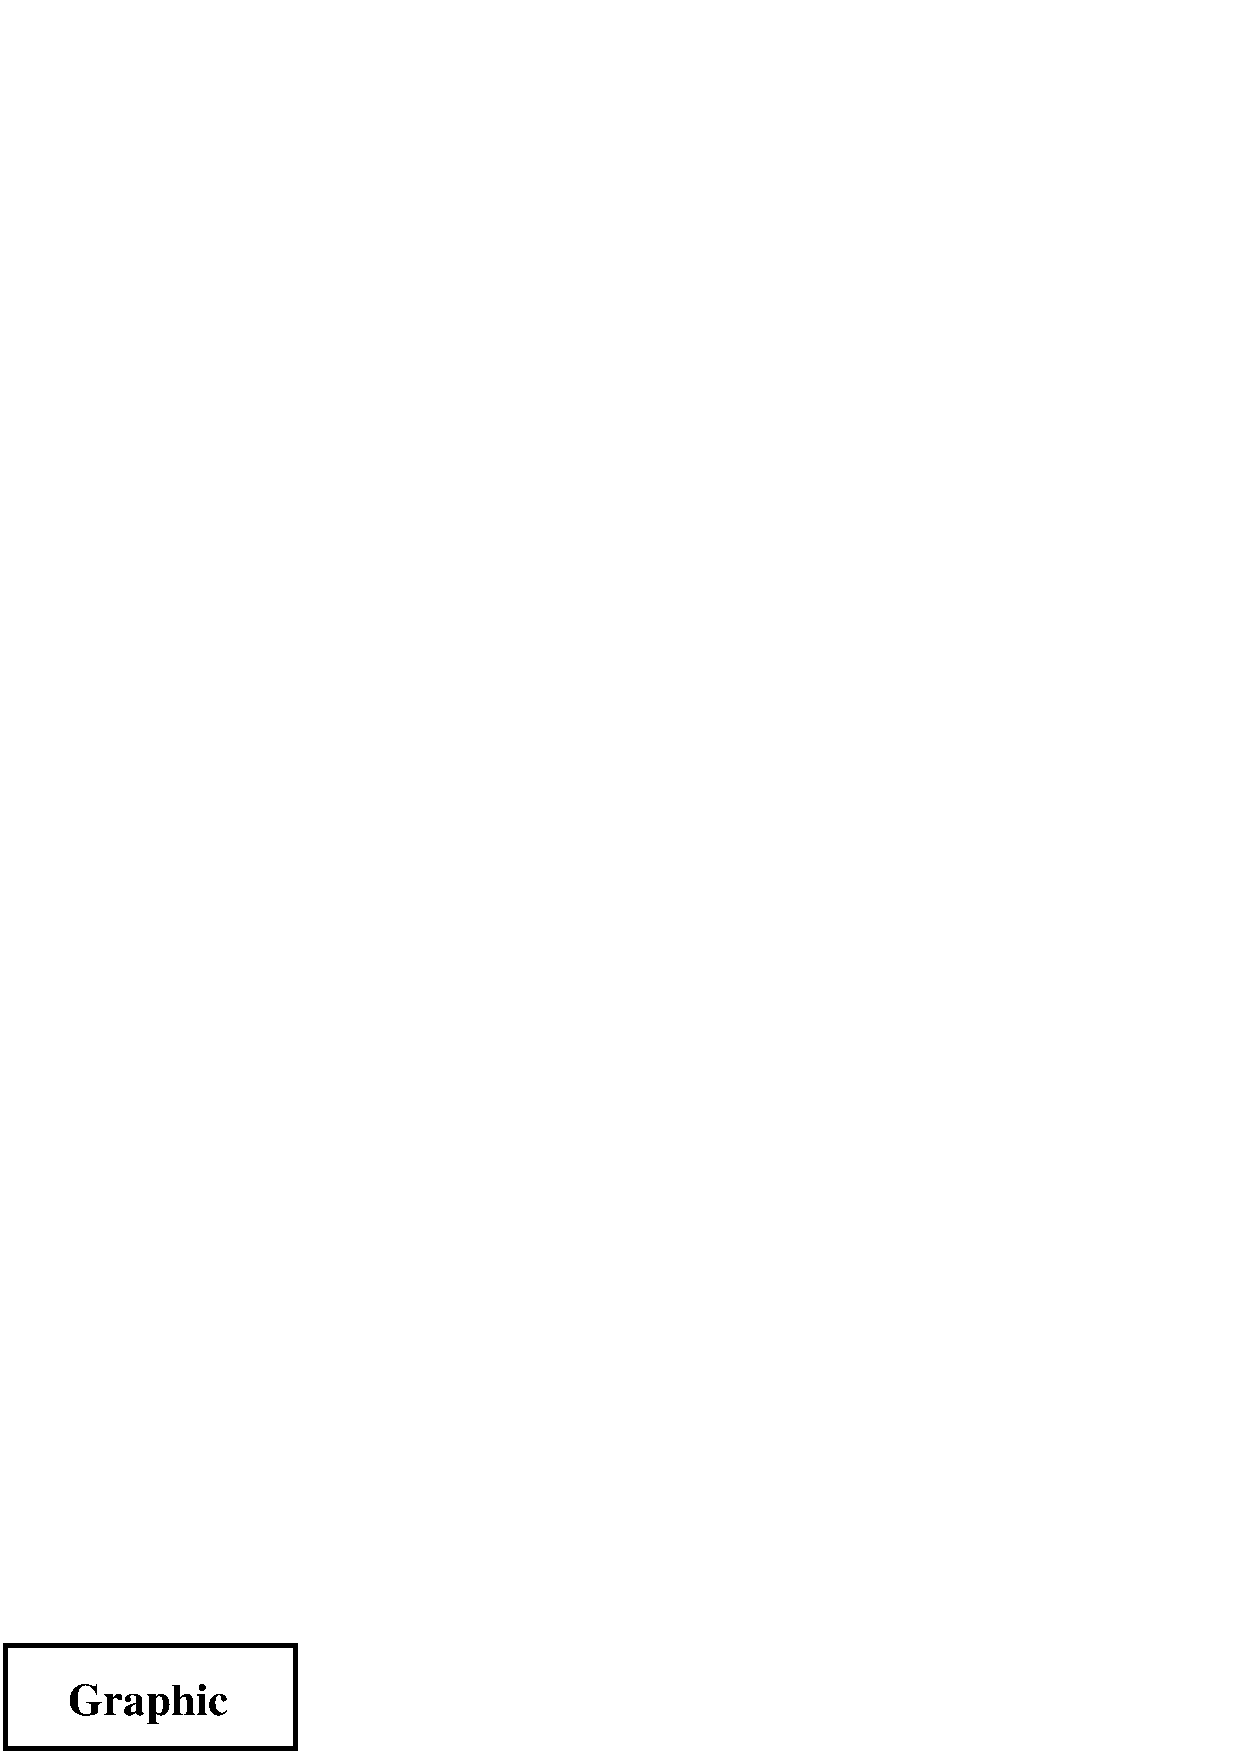
\includegraphics[width=2cm]{graphic}
	\end{minipage}%
	\hspace{1cm}%
	%%----start of second figure graphics----
	\begin{minipage}[b]{.4\linewidth}
		\centering
		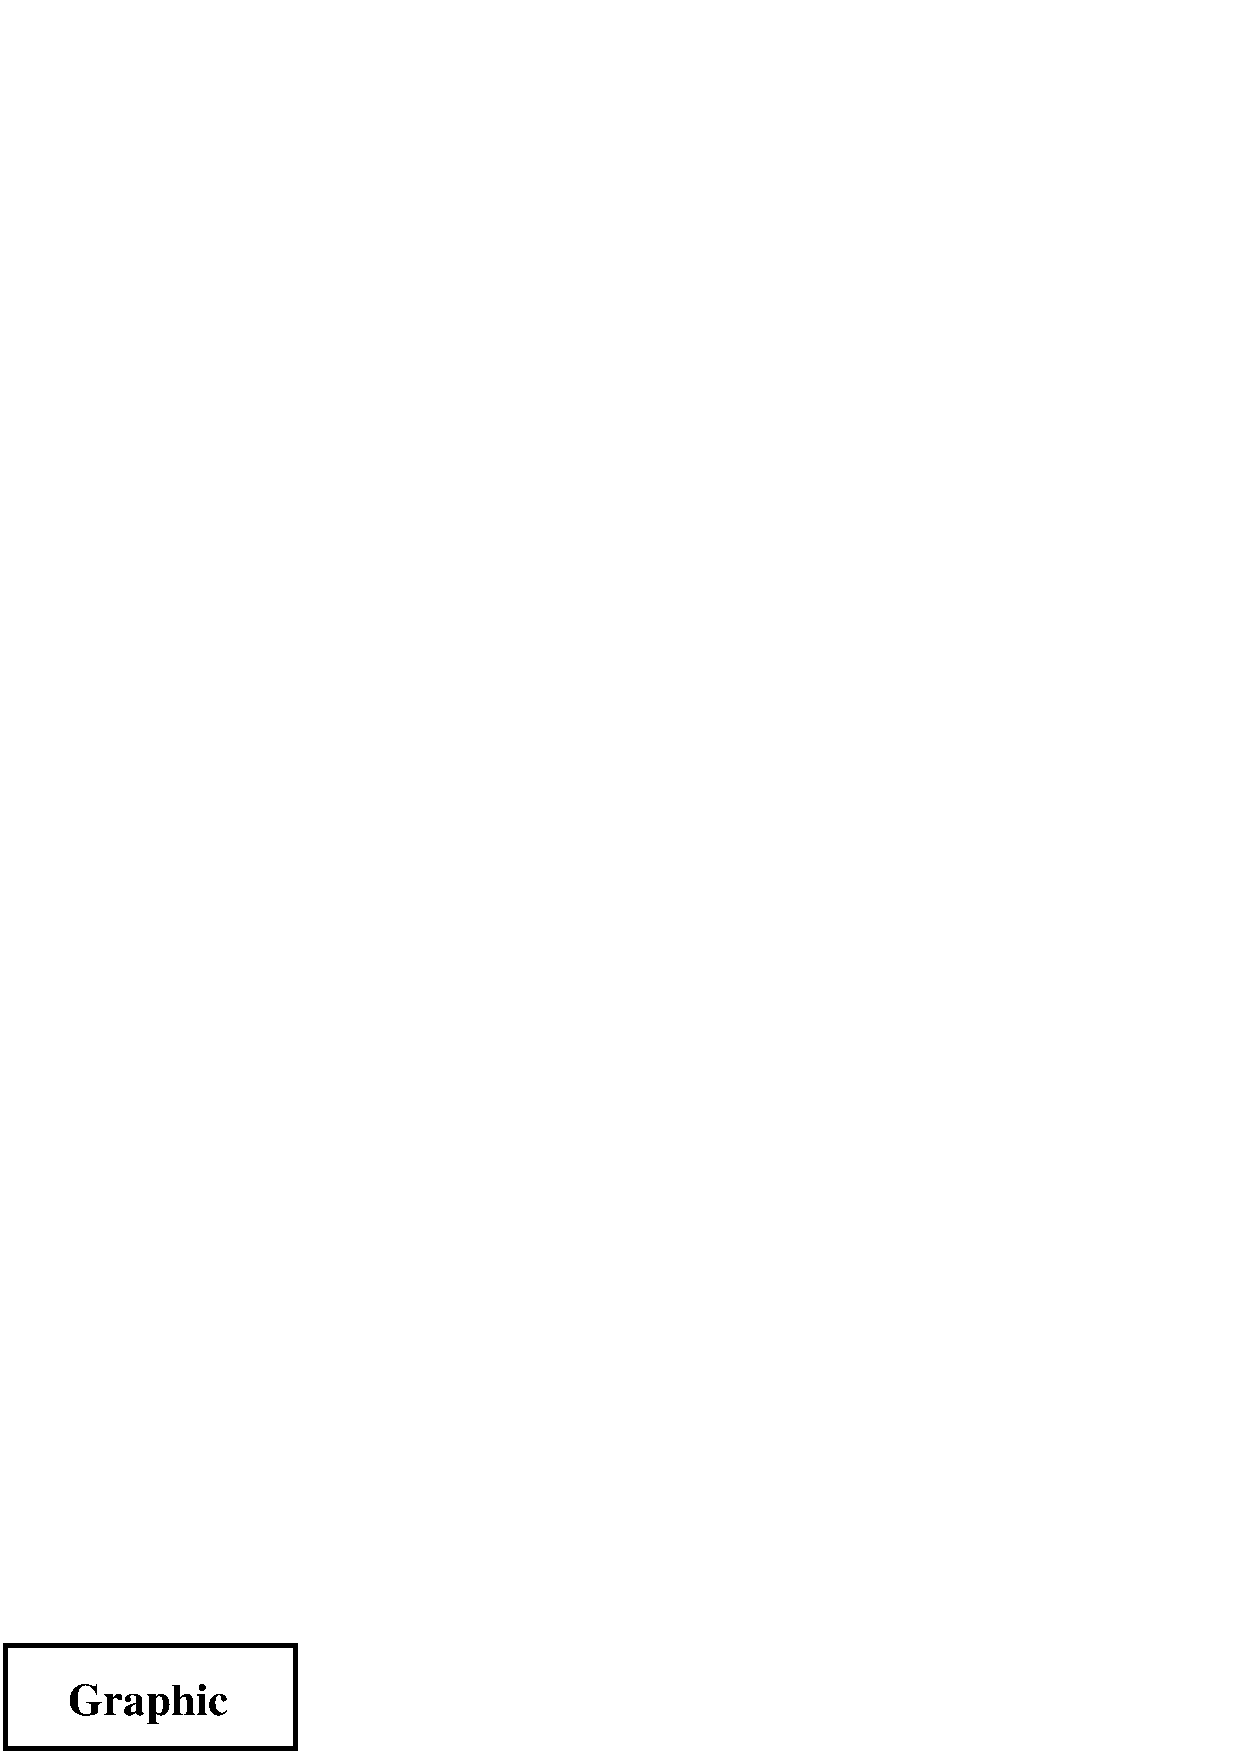
\includegraphics[width=2cm,angle=-30]{graphic}
	\end{minipage}\\[-10pt]
	%%----start of first figure caption----
	\begin{minipage}[t]{.4\linewidth}
		\caption{Box with a Long Caption}\label{fig:mininonrot:a}
	\end{minipage}%
	\hspace{1cm}%
	%%----start of second figure caption----
	\begin{minipage}[t]{.4\linewidth}
		\caption{Rotated Box}\label{fig:minirot:a}
	\end{minipage}%
\end{figure}

在这个例子中,需要注意以下几点:
\begin{itemize}
	\item 在最后一幅图后面用 \cmd{\cmd{}} 来断行,
	\cmd{\cmd{}}的参数项 \opt{[-10pt]} 使得图形与标题之间的距离比当前行距减少10\pt 。
	这样做是让图形和标题更接近些,用户也可自己选用合适的值。
	\item 包含图形的小页使用 \opt{[b]} 选项,使得它们的参考点为其最后一行的基线。
	\item 包含标题小页使用 \opt{[t]} 选项,使得它们的参考点为其第一行的基线,这样使得标题的顶行对齐。
	\item 任何一个 \cmd{label} 命令都必须和它相应的 \cmd{caption} 命令在同一个小页中。
\end{itemize}


\section{图形与表格的平行排列}\label{sec:figuretable}

在第~\ref{sec:sidebyside} 节中,
通过在一个 \env{figure} 环境中使用多个 \cmd{caption} 命令来得到并列的多个图形。
同样地,在一个 \env{table} 环境中使用多个 \cmd{caption} 命令可以得到并列的表格。

第~\ref{sec:nonfloat} 节介绍的 \cmd{captionof} 命令可以将表格放在图形旁边。
例如下面的命令:
\begin{lstlisting}
\begin{figure}[htb]
	\begin{minipage}[b]{0.5\linewidth}
		\centering
		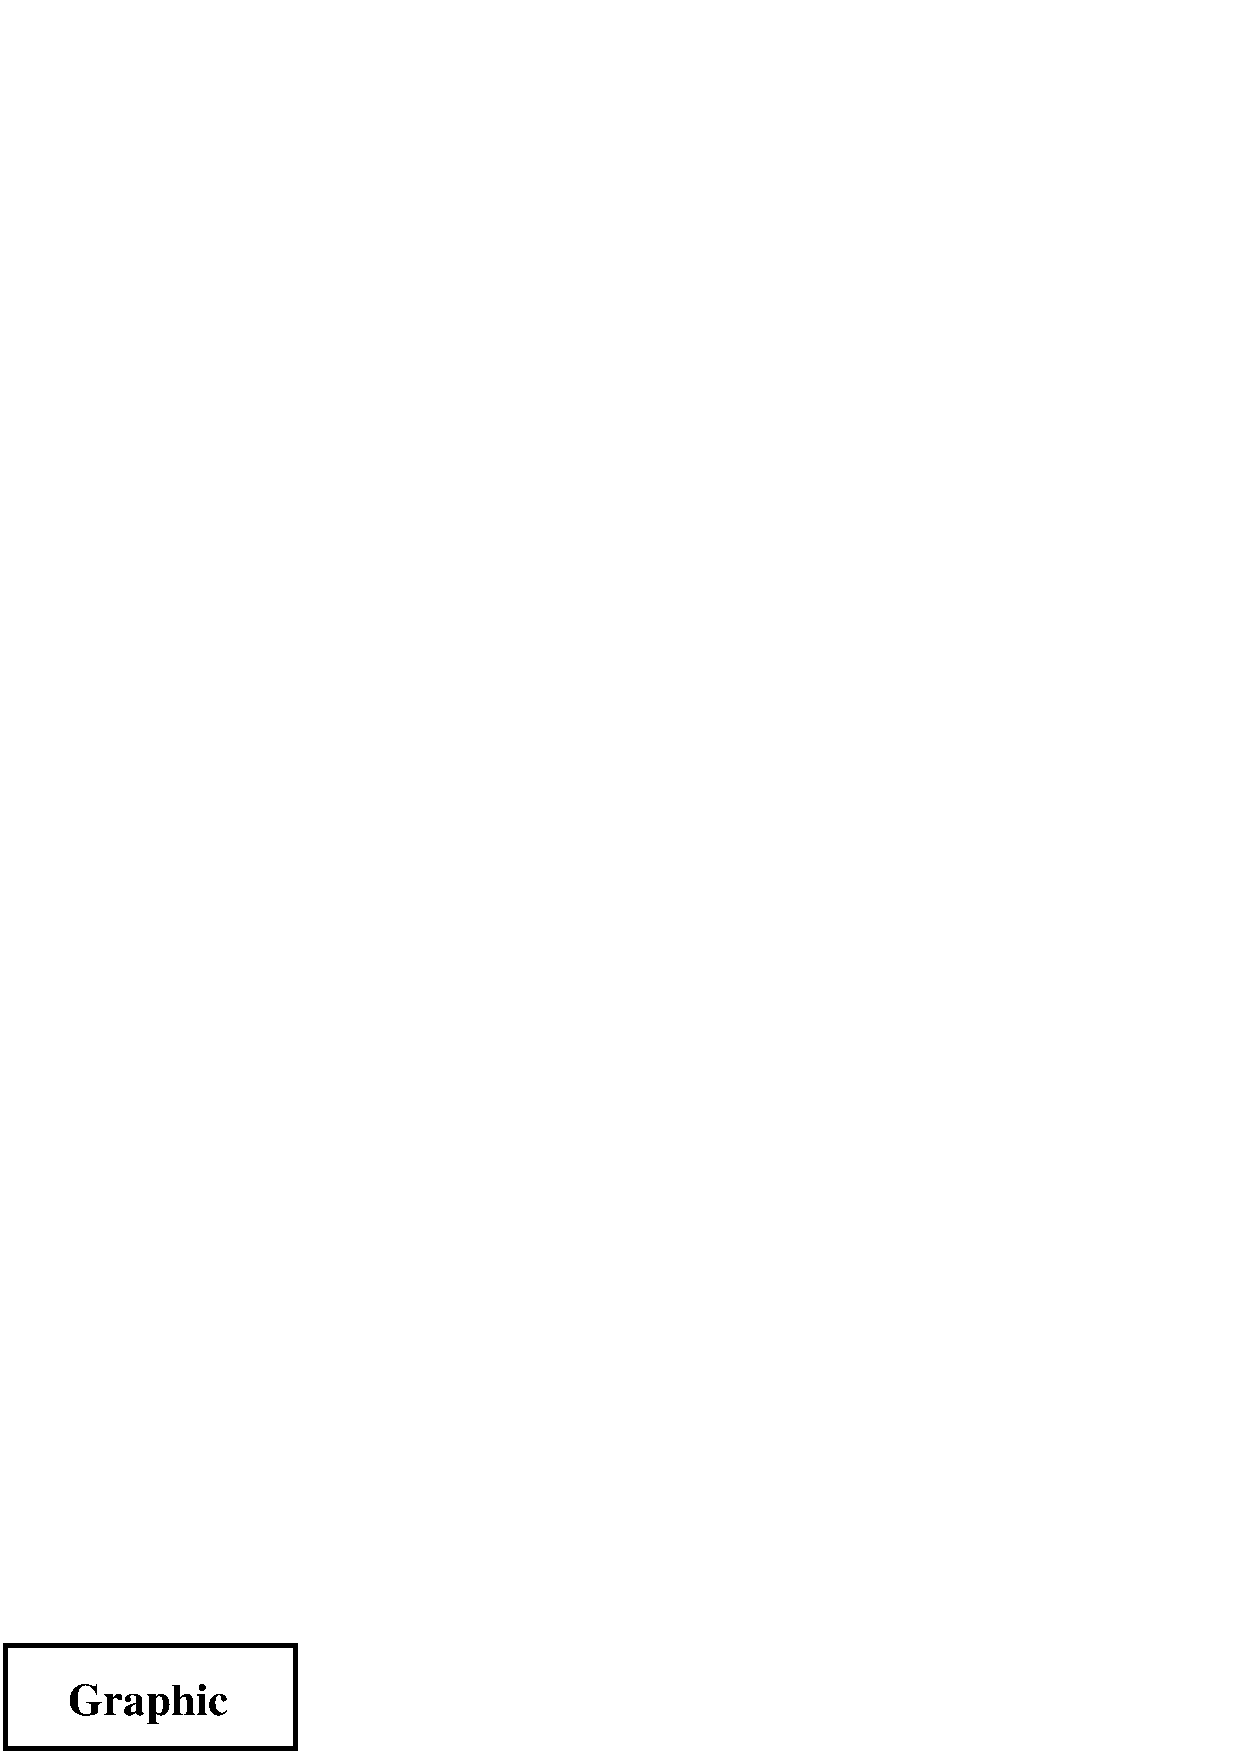
\includegraphics[width=0.8\linewidth]{graphic}
		\caption{This is a Figure by a Table}
		\label{fig:by:table}
	\end{minipage}%
	\begin{minipage}[b]{0.5\linewidth}
		\centering
		\begin{tabular}{|c|c|} \hline
			Day & Data \\ \hline\hline
			Monday & 14.6 \\
			Tuesday & 14.3 \\
			Wednesday & 14.2 \\
			Thursday & 14.5 \\
			Friday & 14.9 \\ \hline
		\end{tabular}
		\captionof{table}{This is a Table by a Figure}
		\label{table:by:fig}
	\end{minipage}
\end{figure}
\end{lstlisting}
使用一个 \env{figure} 环境创建图~\ref{fig:by:table} 和 表~\ref{tab:by:fig}。

\begin{figure}[htb]
	\begin{minipage}[b]{0.5\linewidth}
		\centering
		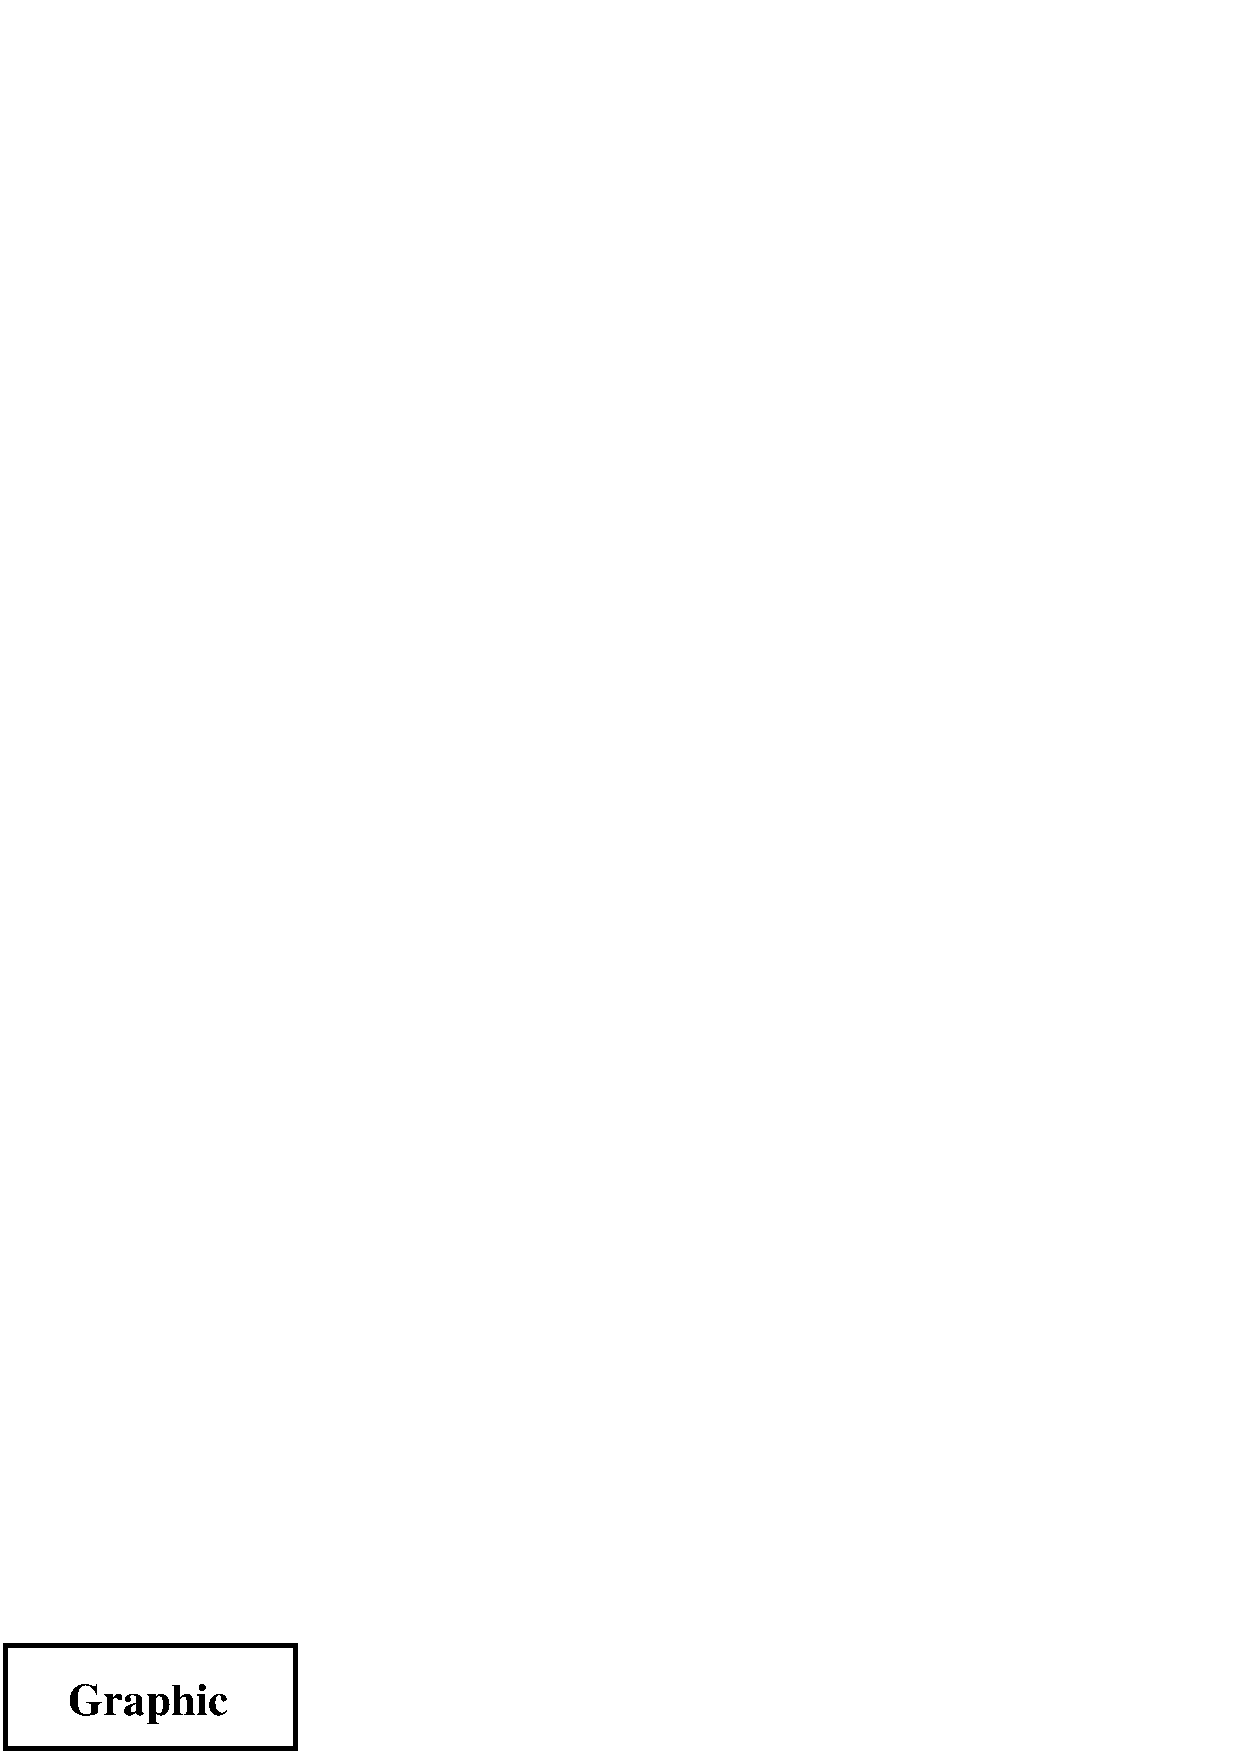
\includegraphics[width=0.8\linewidth]{graphic}
		\caption{This is a Figure by a Table}
		\label{fig:by:table}
	\end{minipage}%
	\begin{minipage}[b]{0.5\linewidth}
		\centering
		\begin{tabular}{|c|c|} \hline
			Day & Data \\ \hline\hline
			Monday & 14.6 \\
			Tuesday & 14.3 \\
			Wednesday & 14.2 \\
			Thursday & 14.5 \\
			Friday & 14.9 \\ \hline
		\end{tabular}
		\captionof{table}{This is a Table by a Figure}
		\label{table:by:fig}
	\end{minipage}
\end{figure}

因为 \LaTeX{} 允许图形的浮动不必考虑其前后表格的顺序,
所以在 \env{figure} 环境中使用
\begin{lstlisting}
\captionof{table}{...}
\end{lstlisting}
可能会将该表格放在未处理的表格之前。
类似地,在 \env{table} 环境中使用
\begin{lstlisting}
\captionof{figure}{...}
\end{lstlisting}
可能会将该图形放在未处理的图形之前。
如果不希望这样,
可以在 \env{figure} 环境之前使用 \cmd{FloatBarrier} 或者 \cmd{clearpage} 命令清除未处理的浮动体
(参见第~\ref{ssec:unprocessfig} 节)。


\section{堆叠的图形和子图}

第~\ref{sec:sidebyside}~节介绍了一系列方法创建并列图形。
这些方法的原理都是将对象(图形、小页、子浮动体等)依次排列在一条直线上。
当使用 \cmd{\cmd{}} 显式断行时,相同的方法也可以生成堆叠的图形。
此外还可以通过 \cmd{\cmd{}} 命令的可选参数(例如 \cmd{\cmd{}}\opt{[20pt]})指定竖直间距。

\subsection{堆叠的图形}

第~\ref{sec:sidebyside}~节介绍了如何创建并列图形。
本节的内容表明,添加断行可以生成多行图形。
例如下列代码
\begin{lstlisting}
\begin{figure}[htbp]
	\centering
	%%----start of first figure----
	\begin{minipage}[t]{0.25\linewidth}
		\centering
		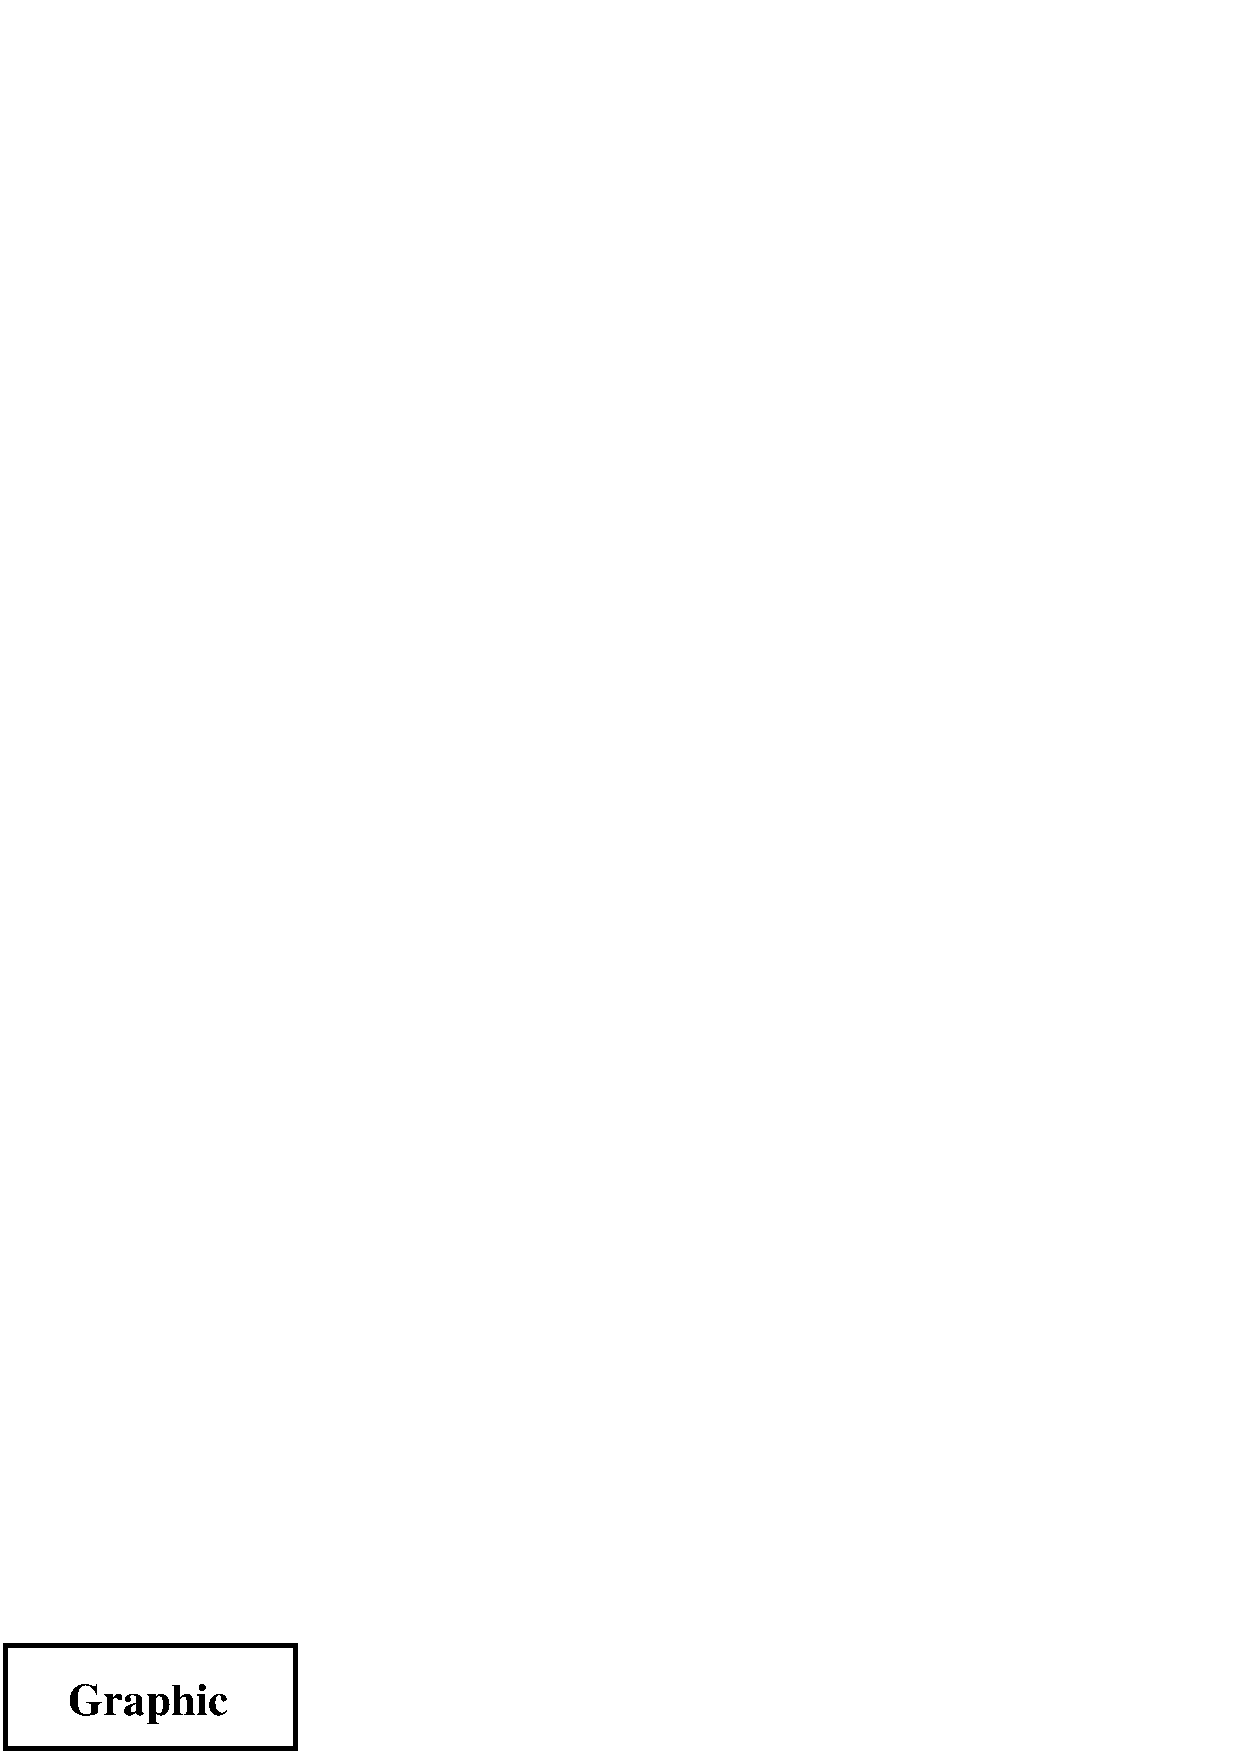
\includegraphics[width=\linewidth]{graphic}
		\caption{First Stacked Figure}
		\label{fig:stacked:first}
	\end{minipage}%
	\hspace{1cm}%
	%%----start of second figure----
	\begin{minipage}[t]{0.25\linewidth}
		\centering
		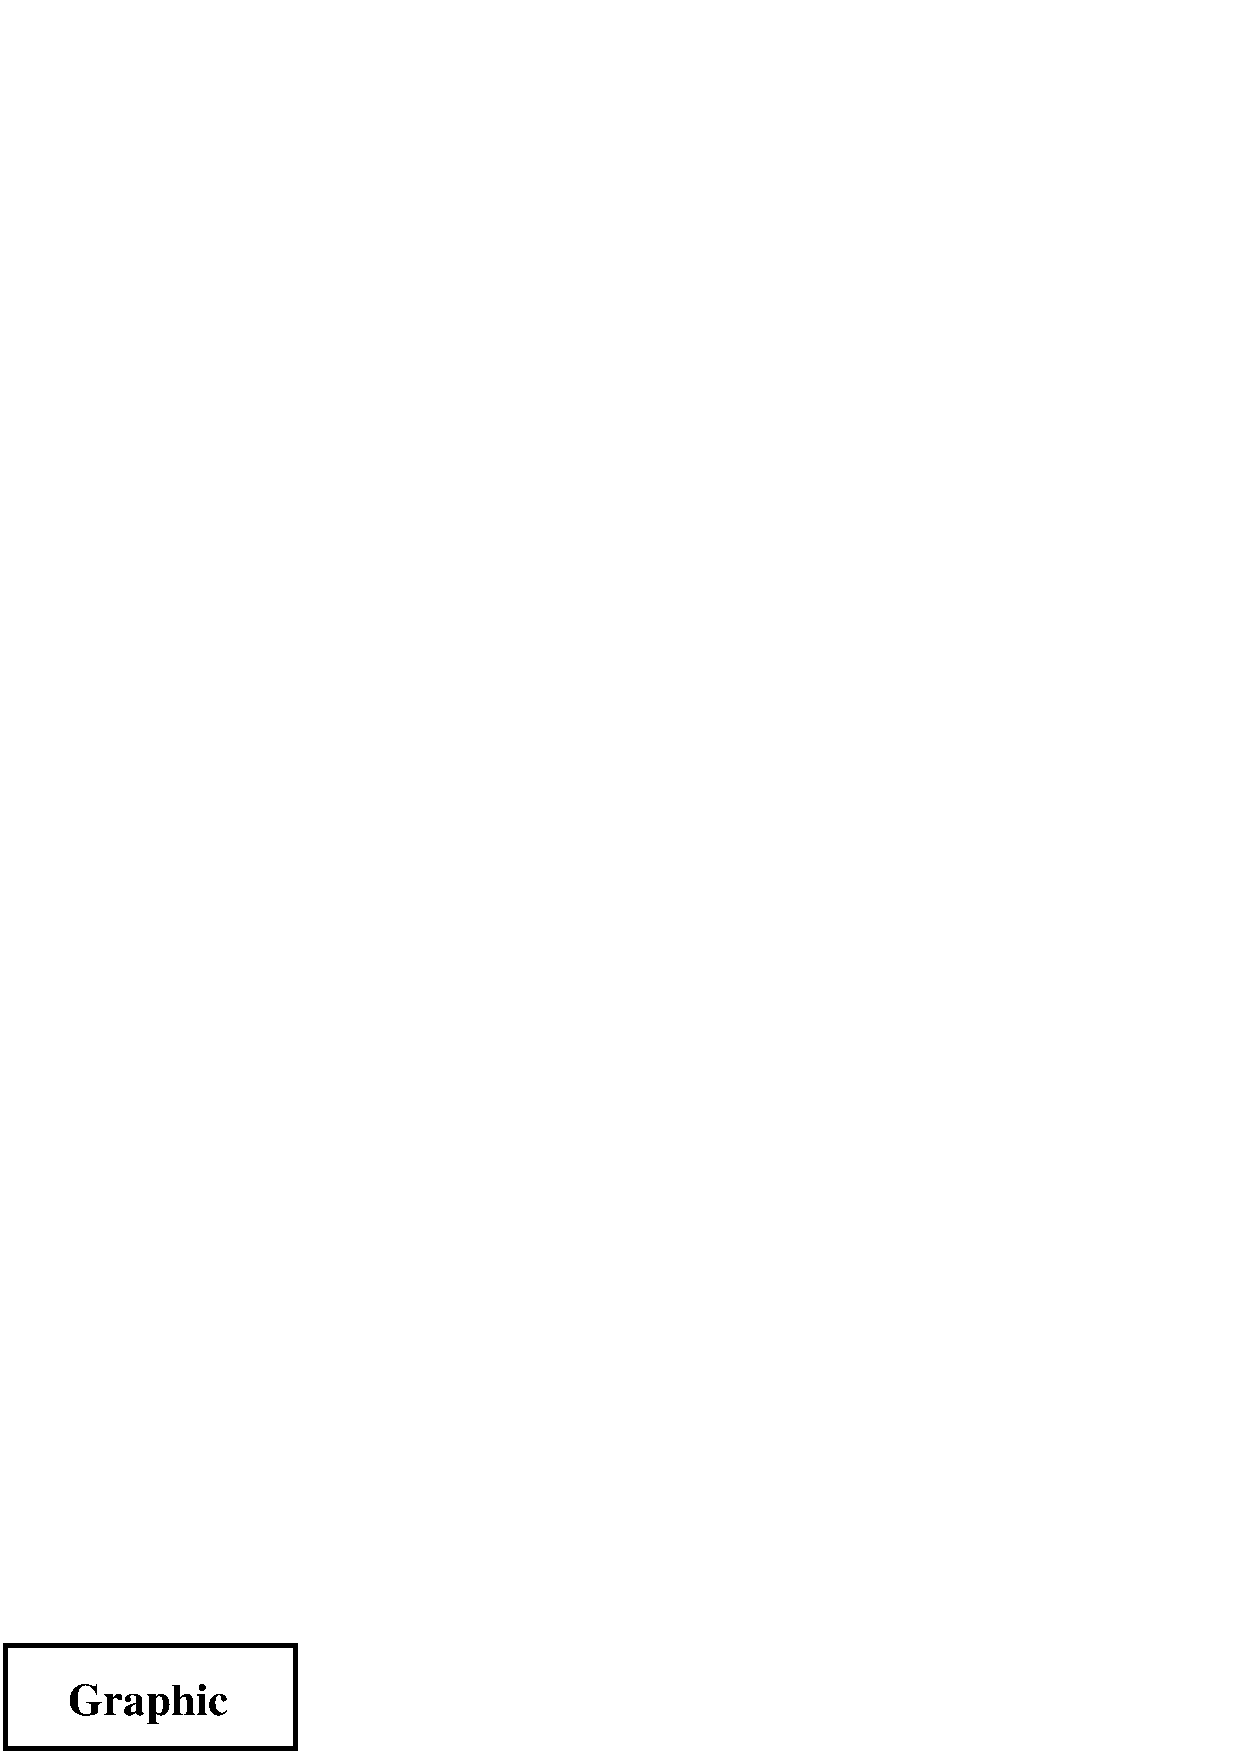
\includegraphics[width=\linewidth]{graphic}
		\caption{Second Stacked Figure}
		\label{fig:stacked:second}
	\end{minipage}\\[20pt]
	%%----start of third figure----
	\begin{minipage}[t]{0.25\linewidth}
		\centering
		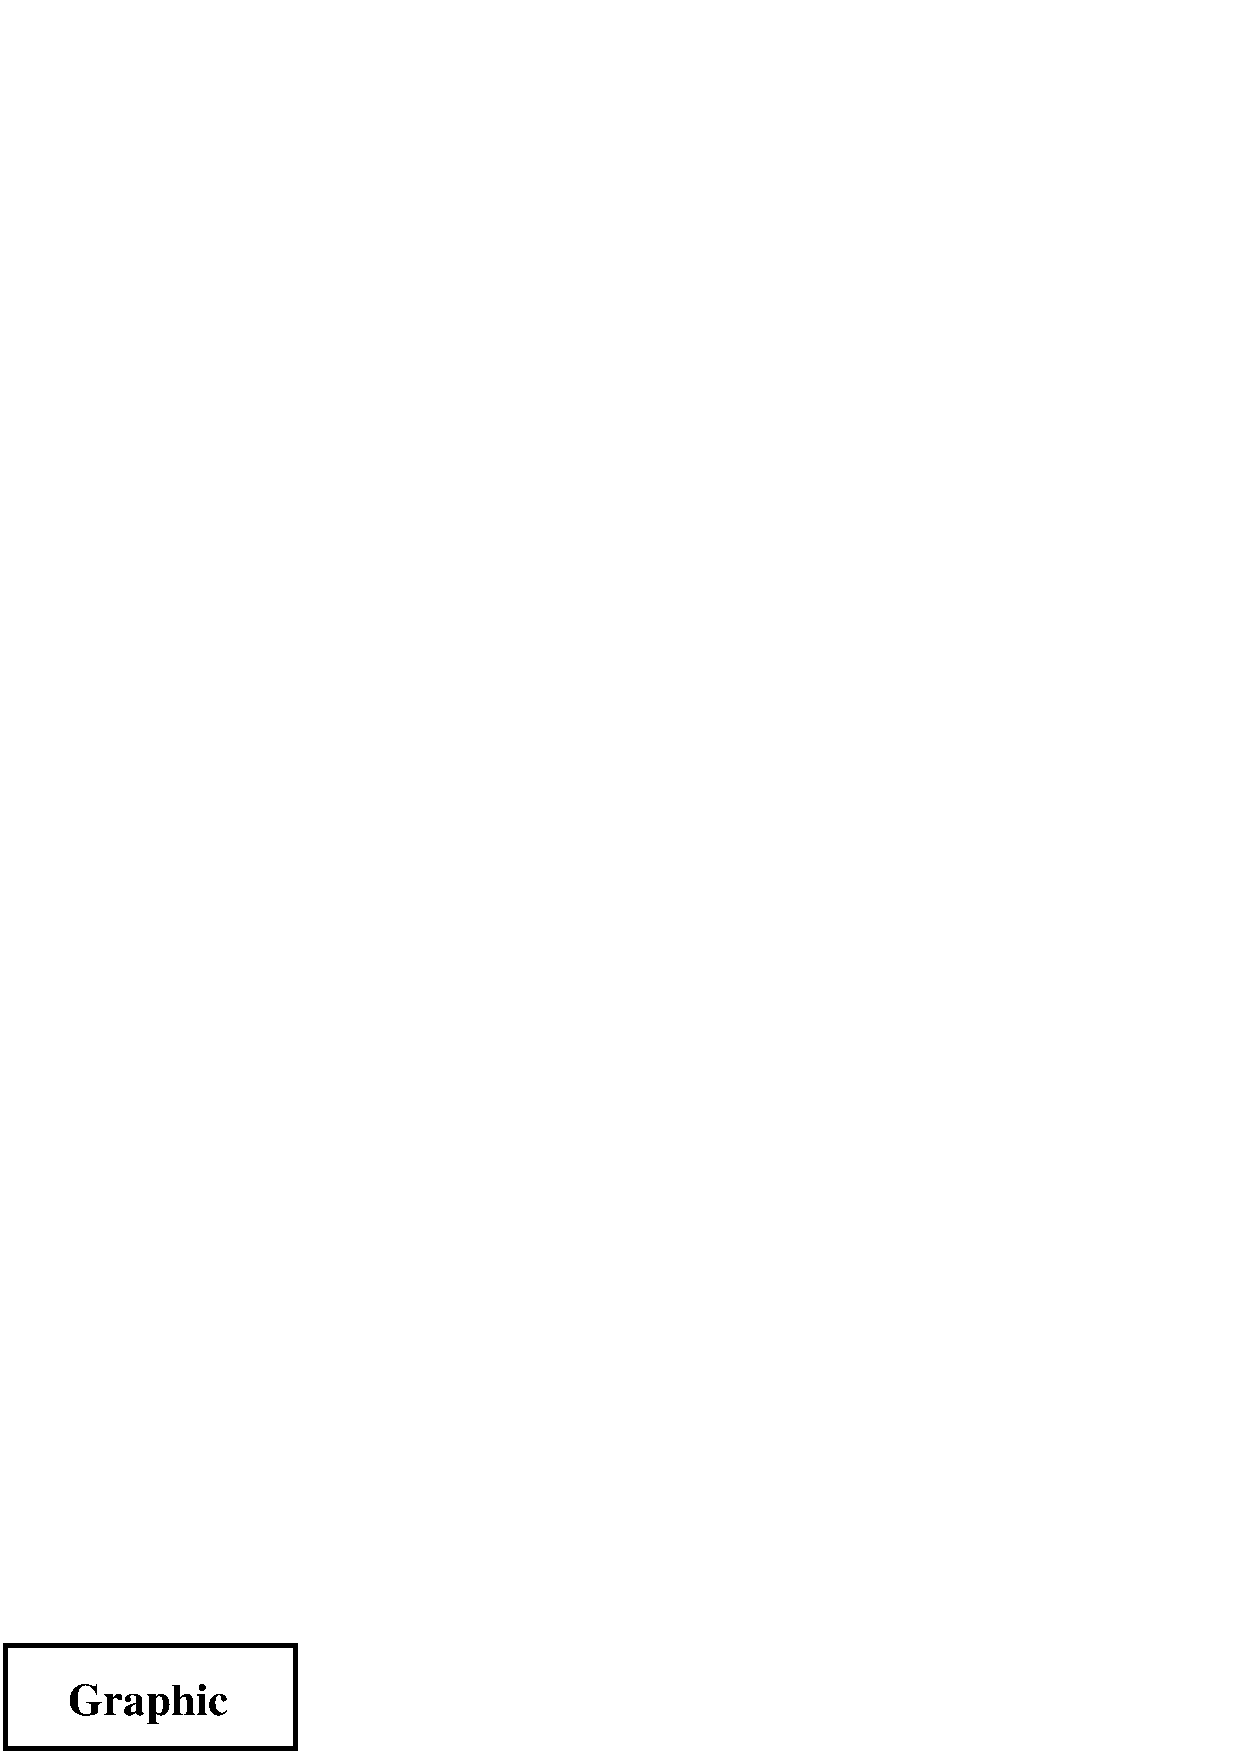
\includegraphics[width=\linewidth]{graphic}
		\caption{Third Stacked Figure}
		\label{fig:stacked:third}
	\end{minipage}%
	\hspace{1cm}%
	%%----start of fourth figure----
	\begin{minipage}[t]{0.25\linewidth}
		\centering
		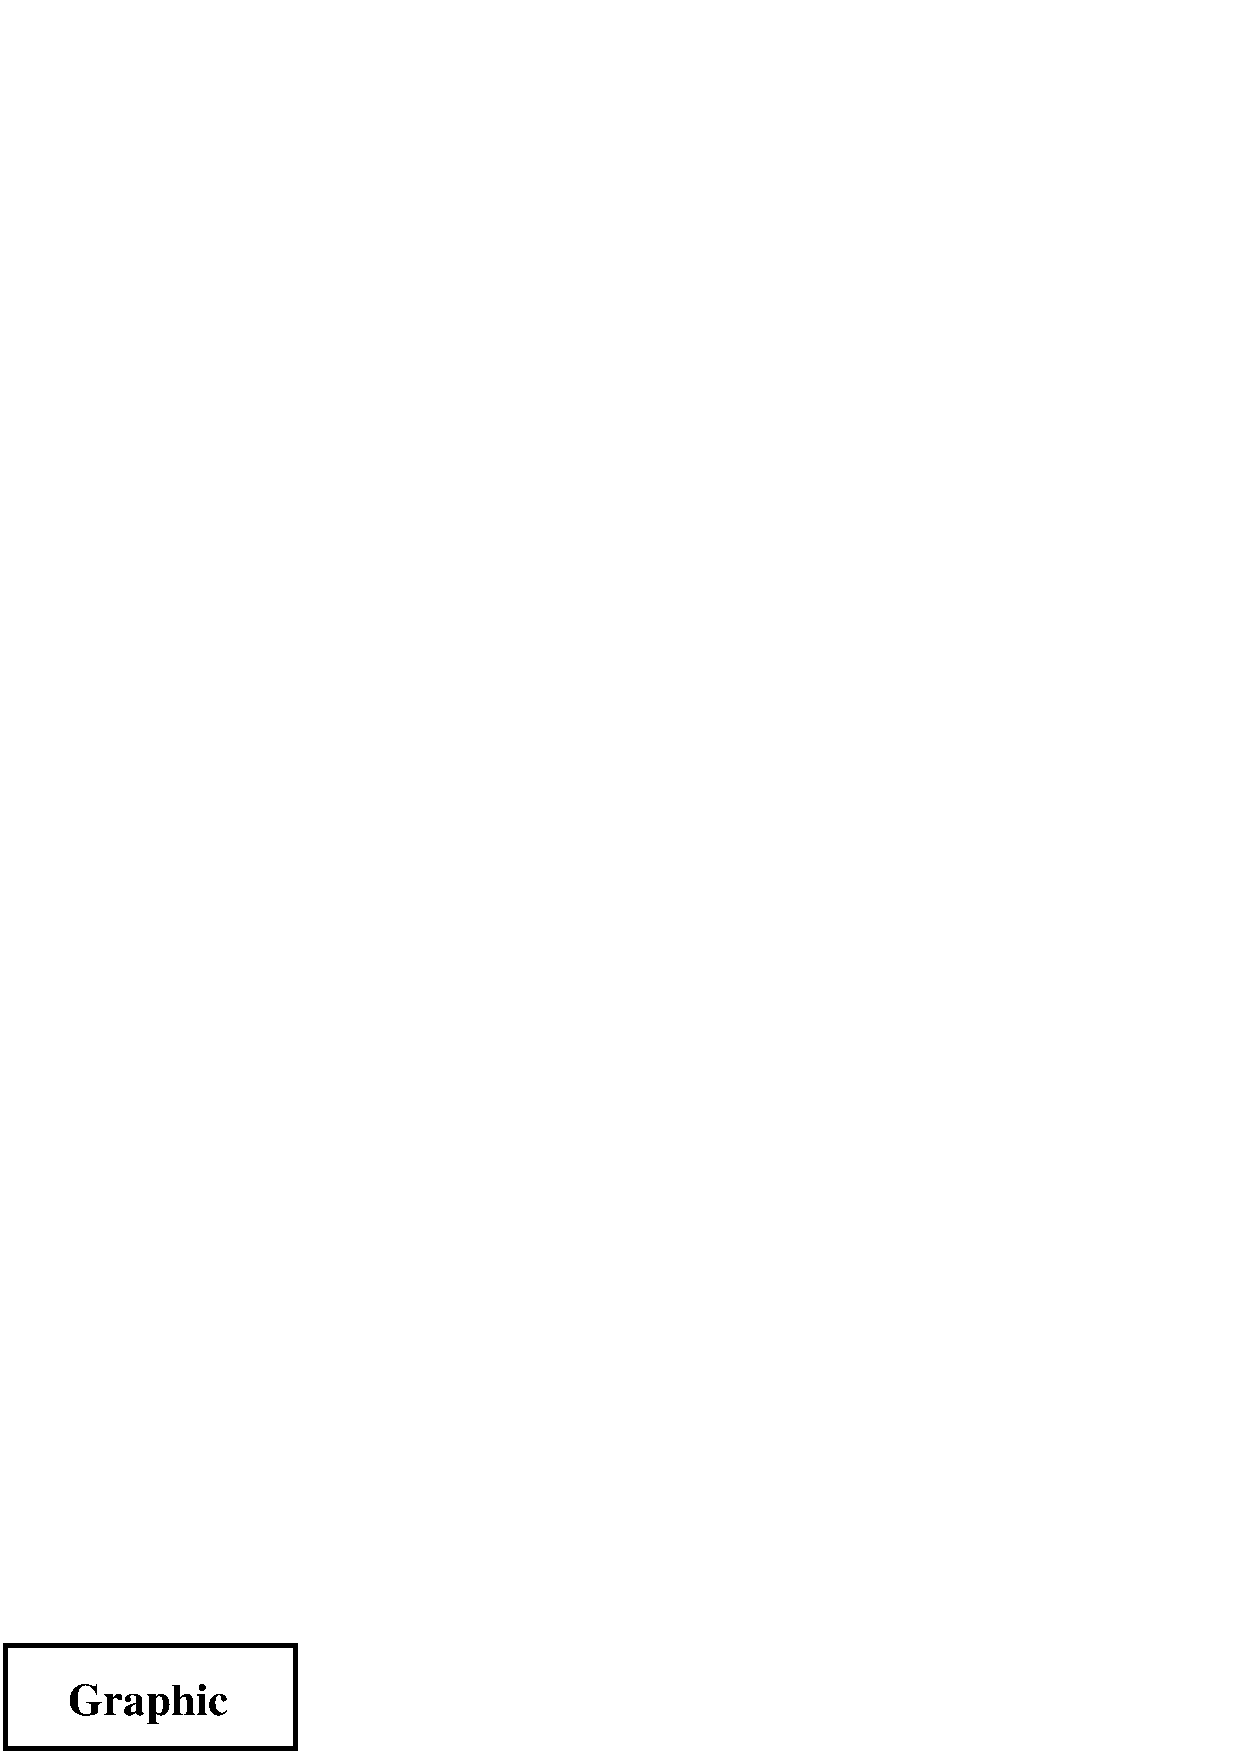
\includegraphics[width=\linewidth]{graphic}
		\caption{Fourth Stacked Figure}
		\label{fig:stacked:fourth}
	\end{minipage}%
	\hspace{1cm}%
	%%----start of fifth figure----
	\begin{minipage}[t]{0.25\linewidth}
		\centering
		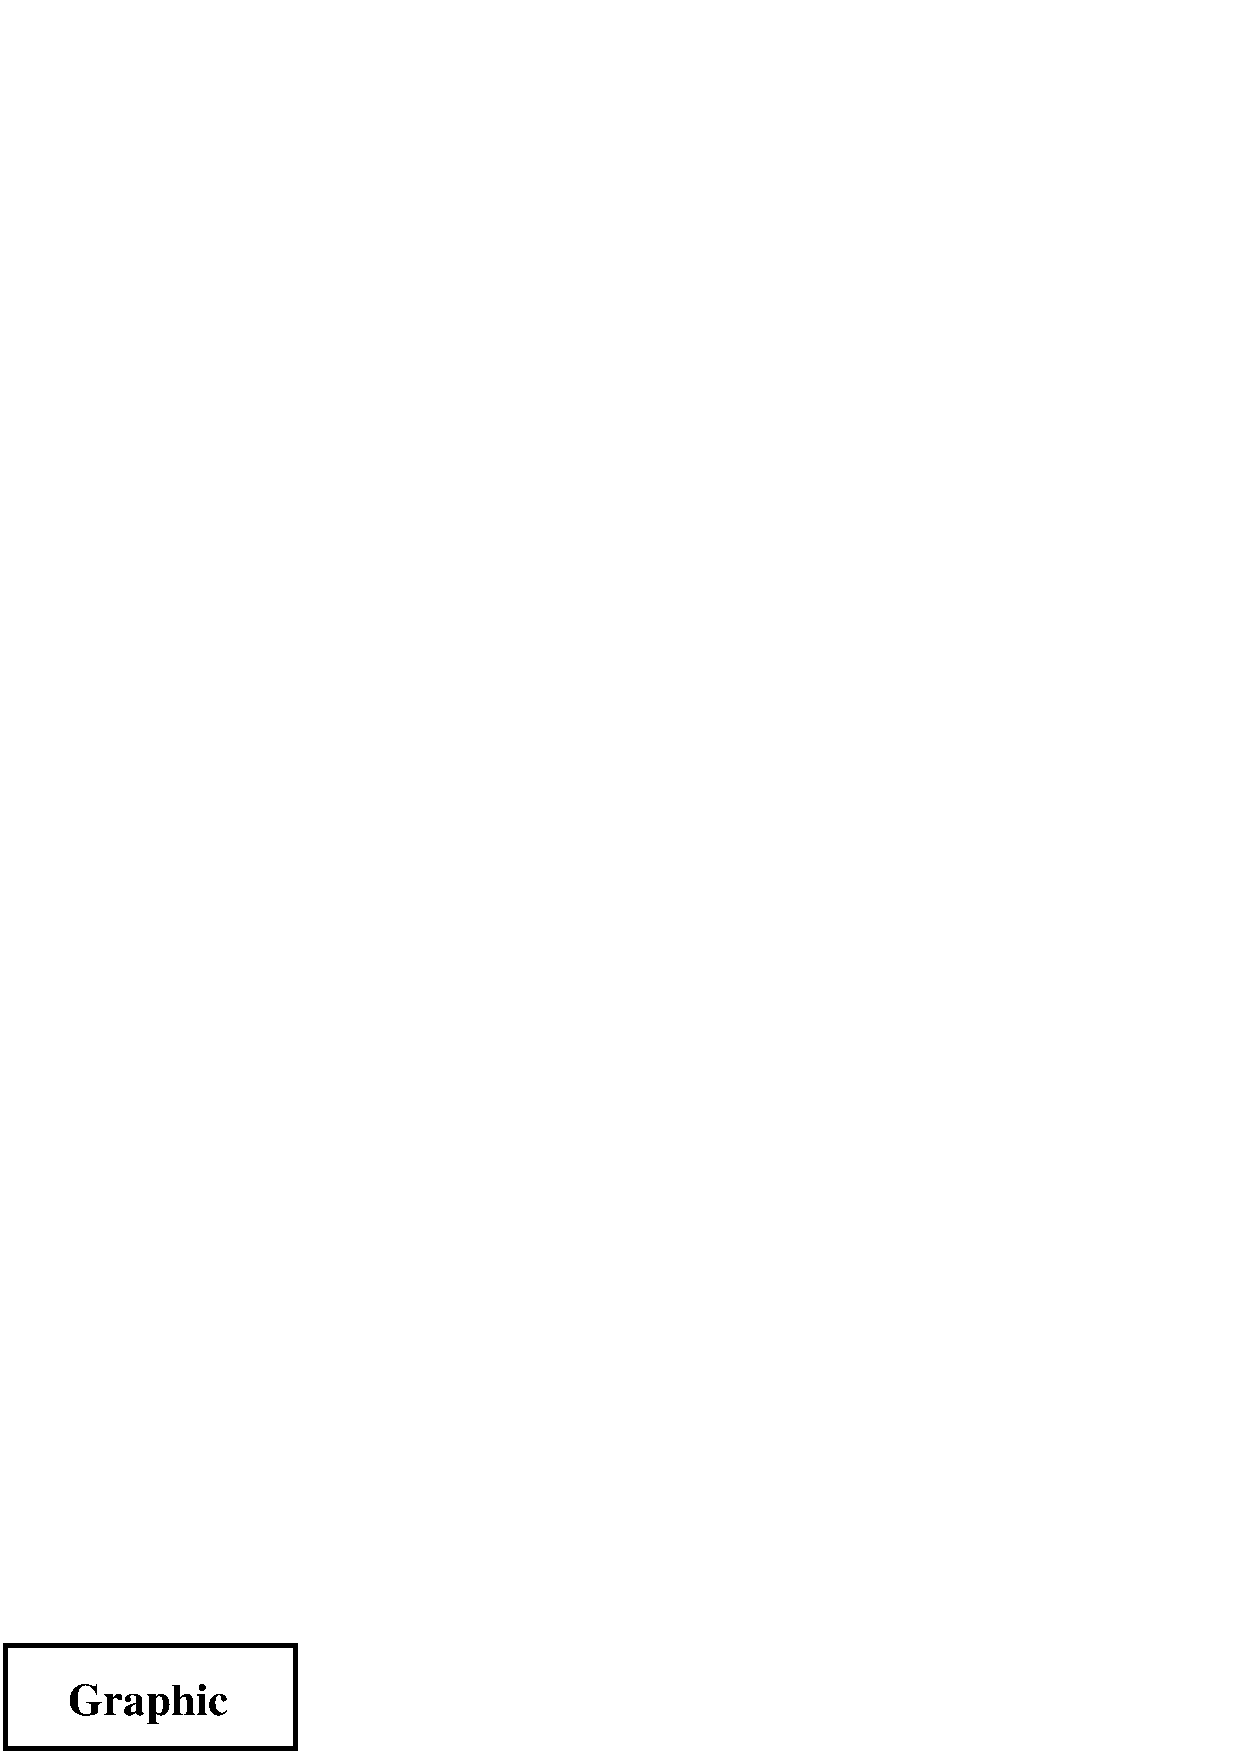
\includegraphics[width=\linewidth]{graphic}
		\caption{Fifth Stacked Figure}
		\label{fig:stacked:fifth}
	\end{minipage}%
\end{figure}
\end{lstlisting}
生成一组图~\ref{fig:stacked:first}--\ref{fig:stacked:fifth}。

\begin{figure}[htbp]
	\centering
	%%----start of first figure----
	\begin{minipage}[t]{0.25\linewidth}
		\centering
		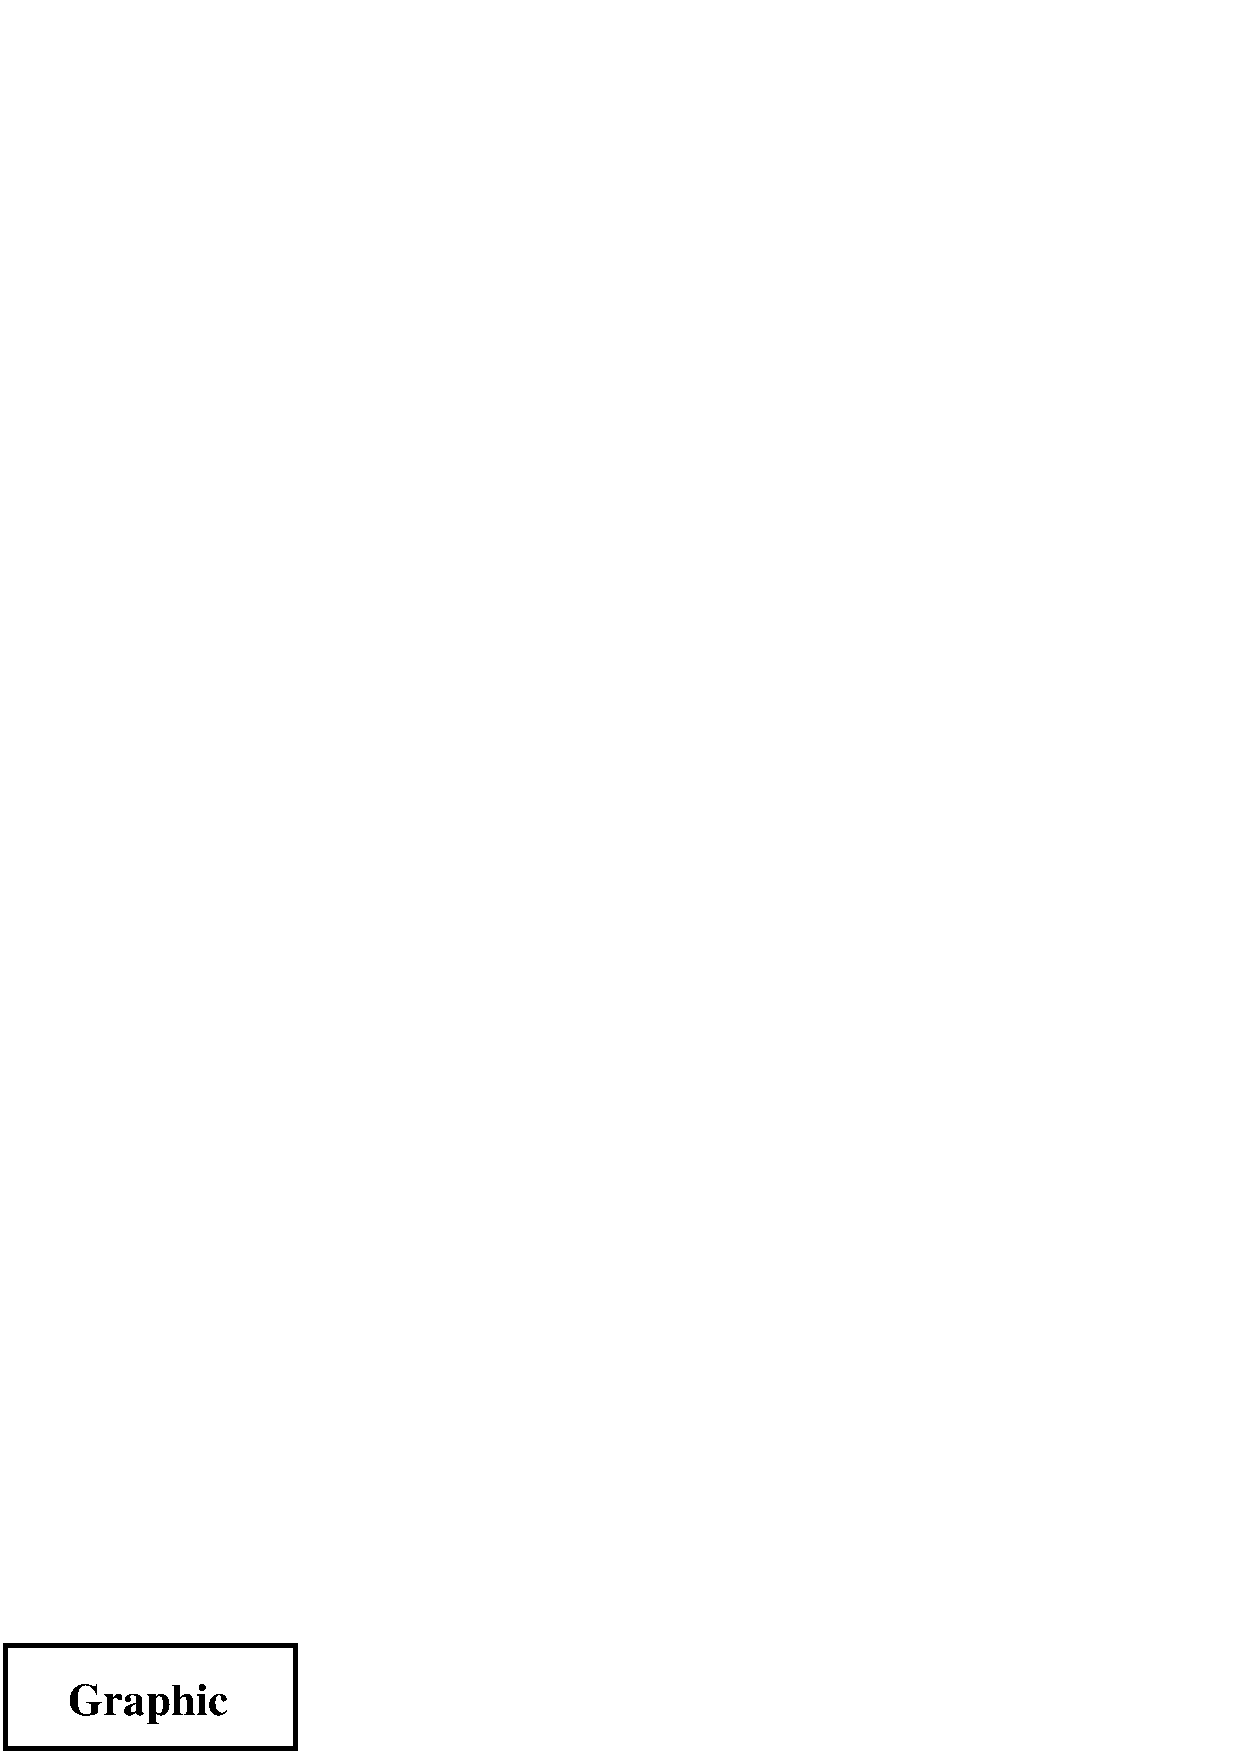
\includegraphics[width=\linewidth]{graphic}
		\caption{First Stacked Figure}
		\label{fig:stacked:first}
	\end{minipage}%
	\hspace{1cm}%
	%%----start of second figure----
	\begin{minipage}[t]{0.25\linewidth}
		\centering
		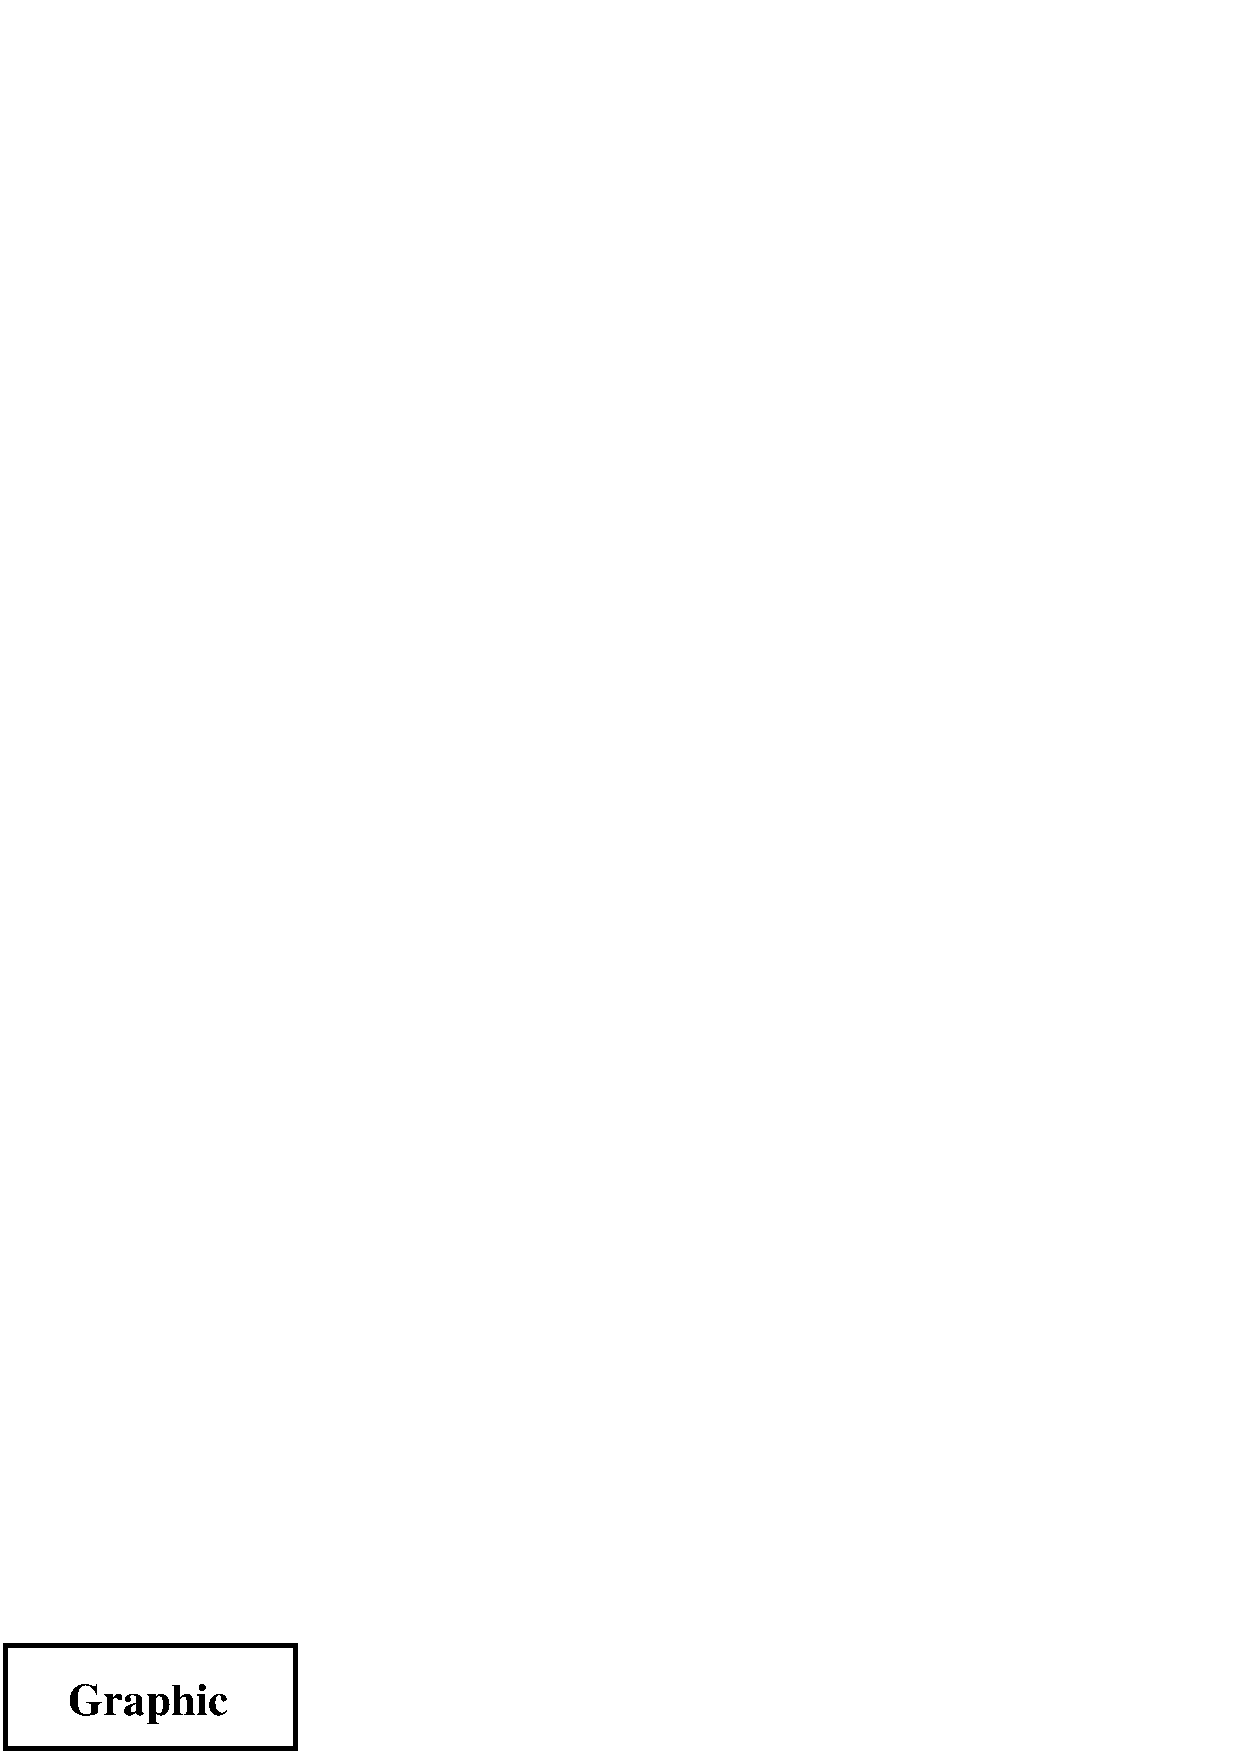
\includegraphics[width=\linewidth]{graphic}
		\caption{Second Stacked Figure}
		\label{fig:stacked:second}
	\end{minipage}\\[20pt]
	%%----start of third figure----
	\begin{minipage}[t]{0.25\linewidth}
		\centering
		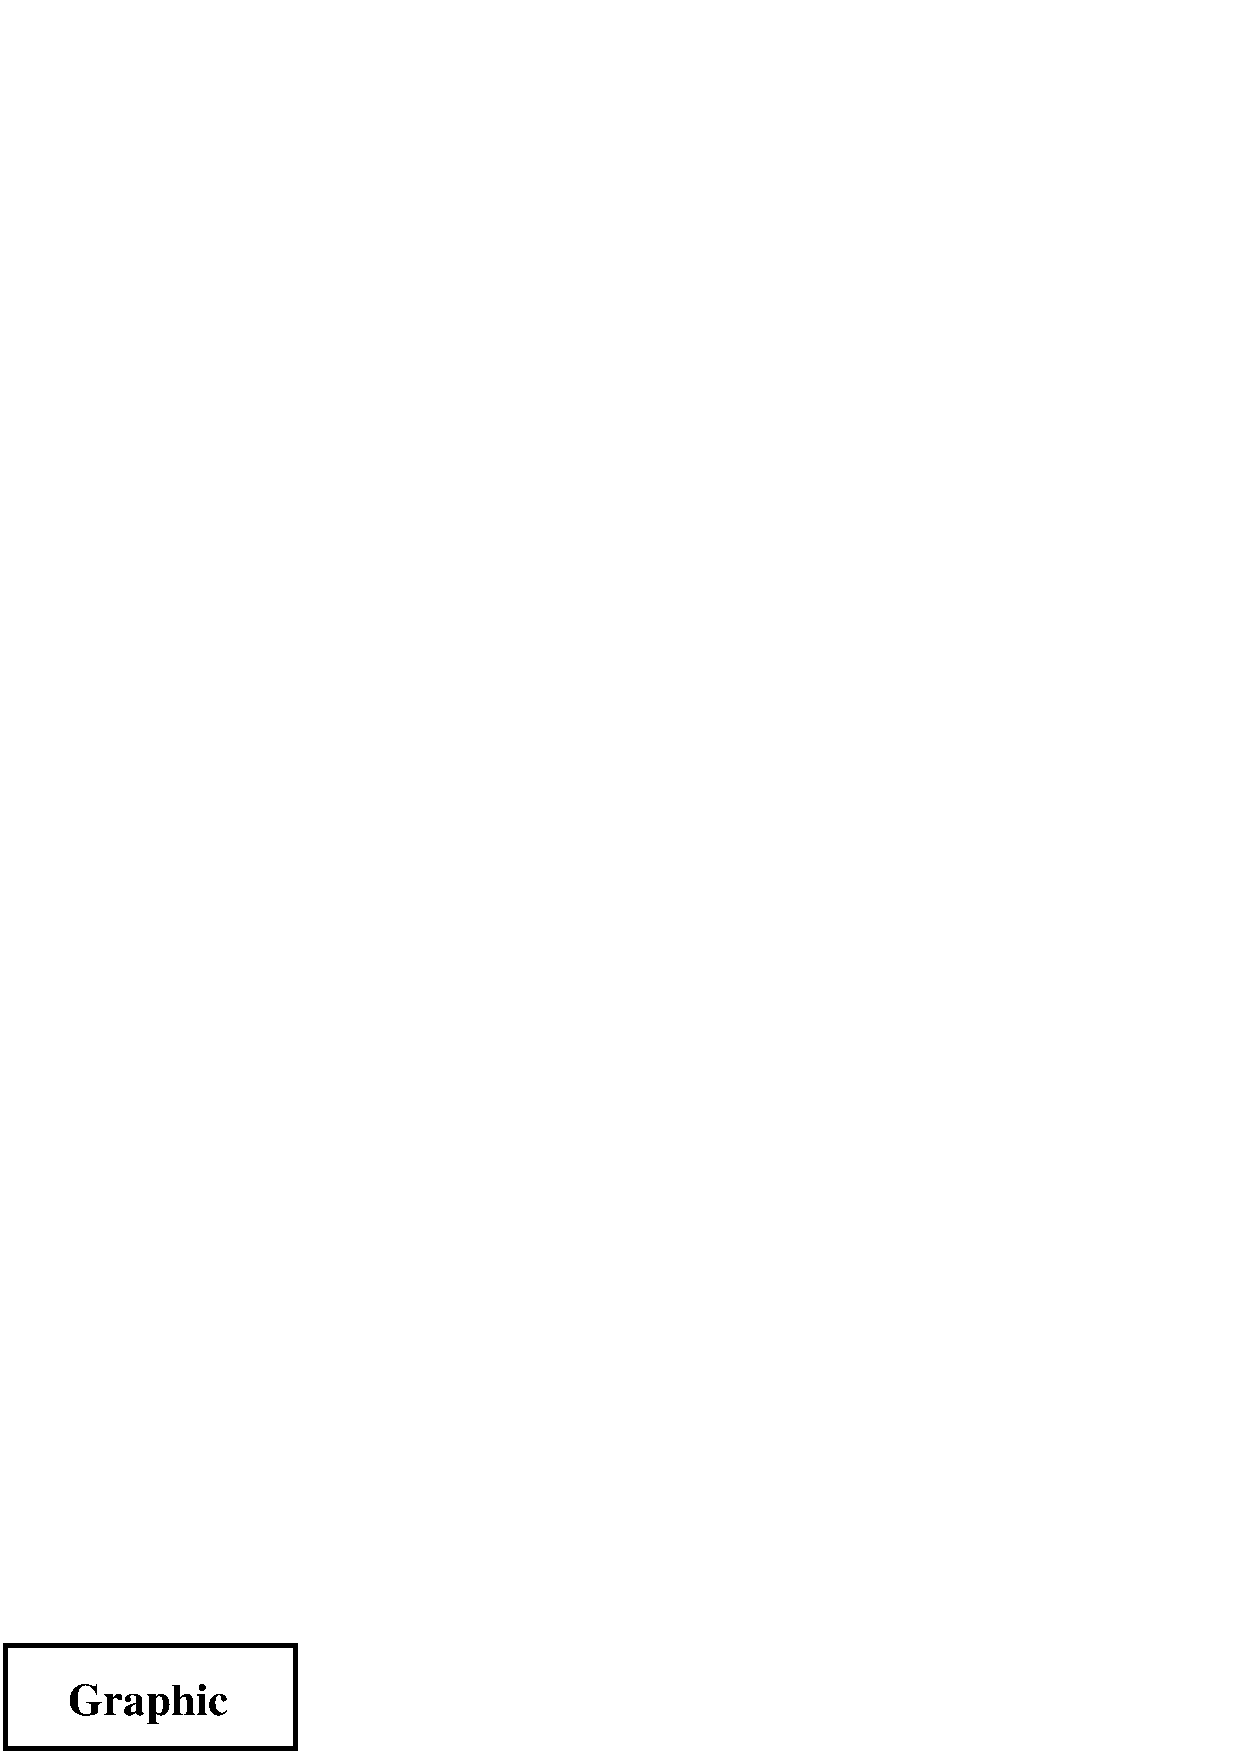
\includegraphics[width=\linewidth]{graphic}
		\caption{Third Stacked Figure}
		\label{fig:stacked:third}
	\end{minipage}%
	\hspace{1cm}%
	%%----start of fourth figure----
	\begin{minipage}[t]{0.25\linewidth}
		\centering
		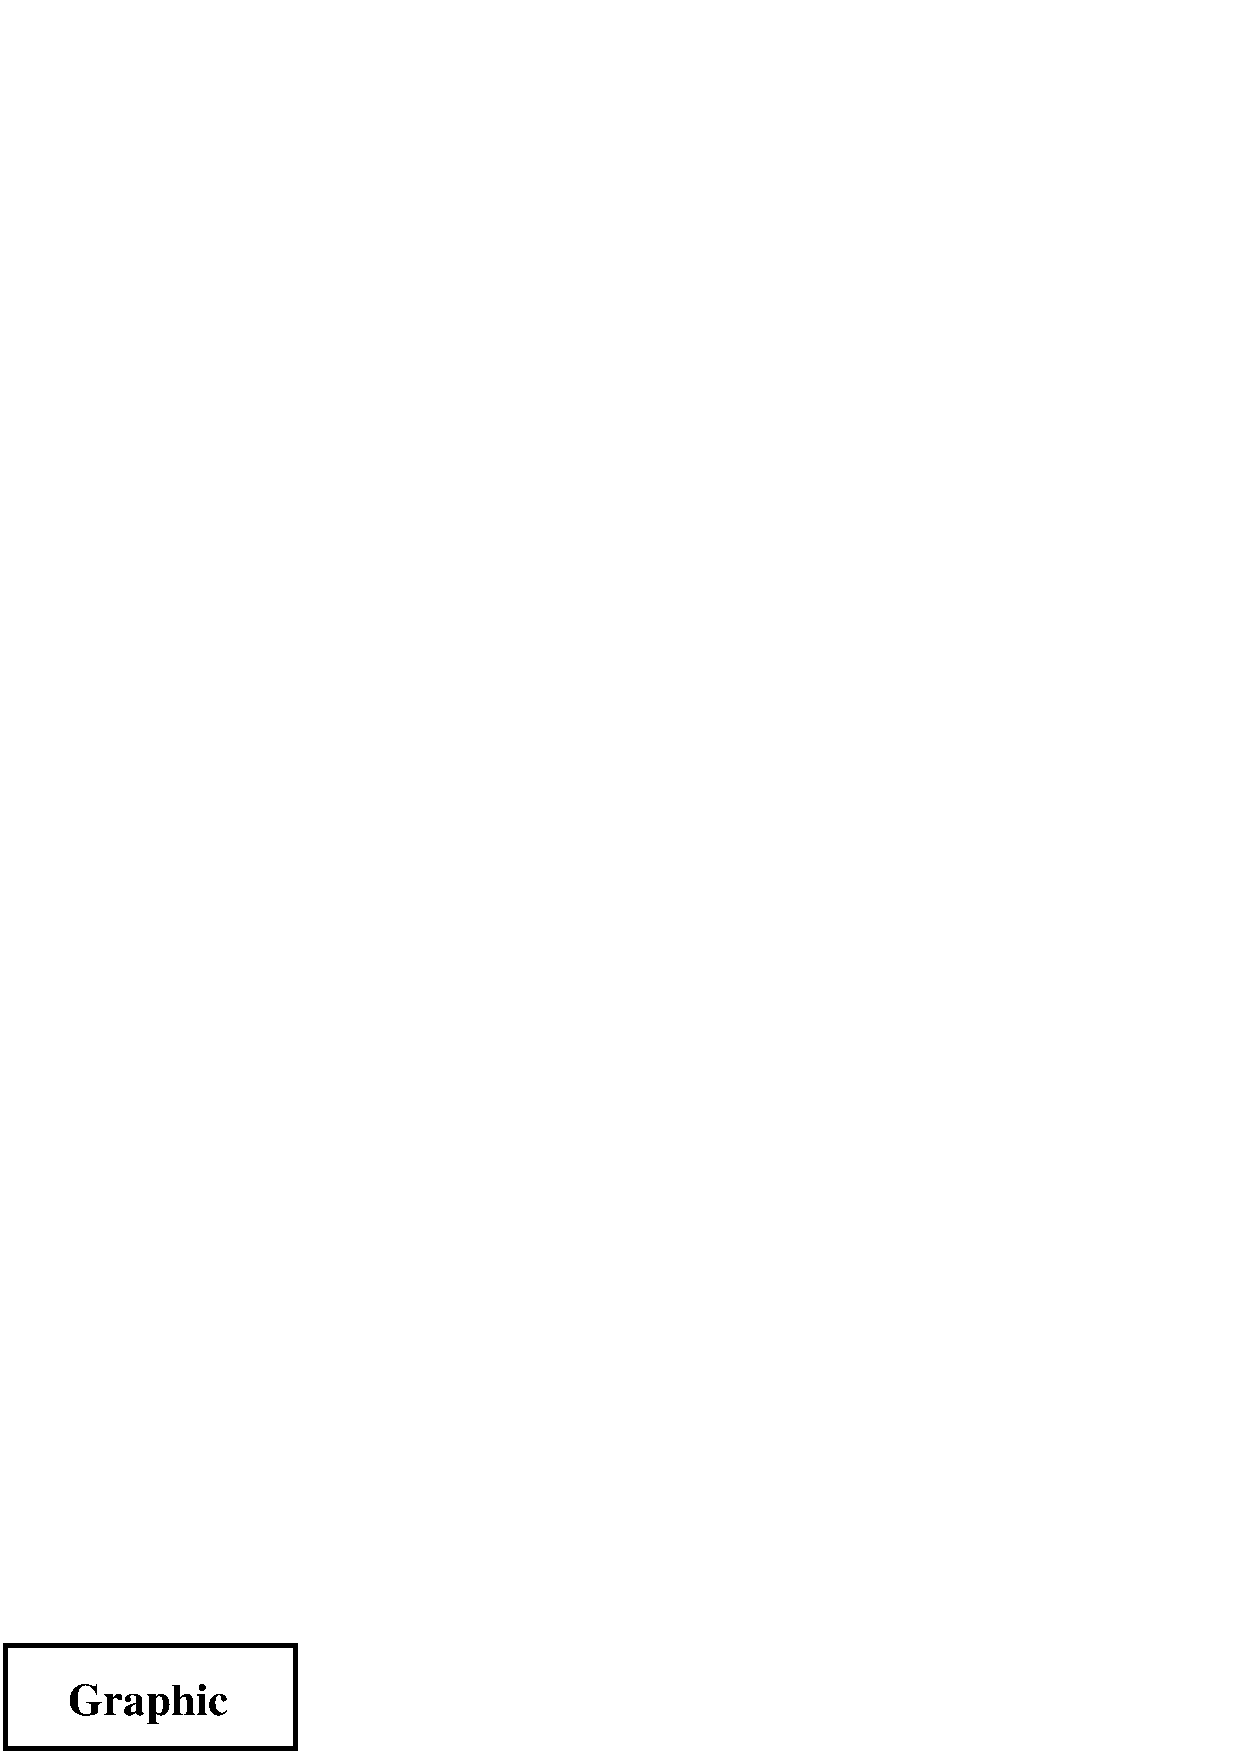
\includegraphics[width=\linewidth]{graphic}
		\caption{Fourth Stacked Figure}
		\label{fig:stacked:fourth}
	\end{minipage}%
	\hspace{1cm}%
	%%----start of fifth figure----
	\begin{minipage}[t]{0.25\linewidth}
		\centering
		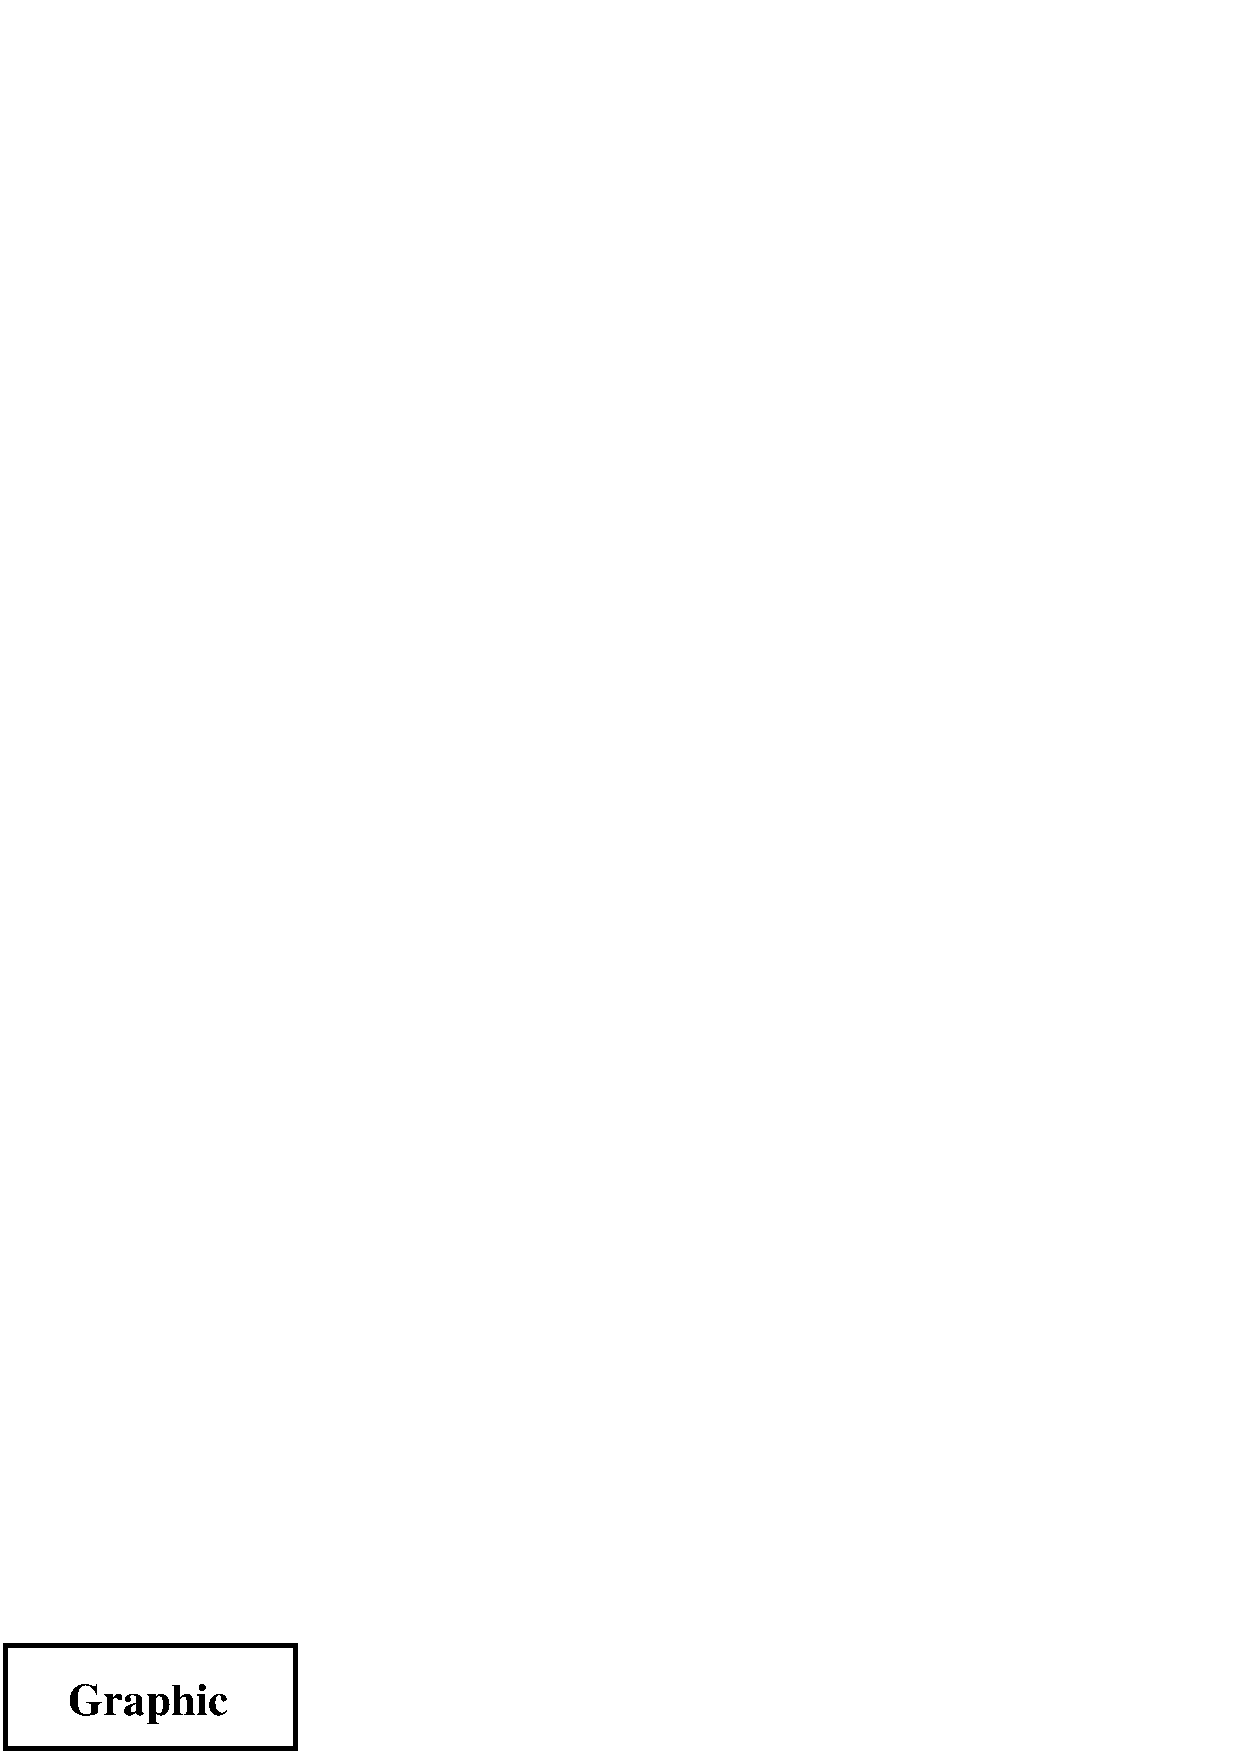
\includegraphics[width=\linewidth]{graphic}
		\caption{Fifth Stacked Figure}
		\label{fig:stacked:fifth}
	\end{minipage}%
\end{figure}

\subsection{堆叠的子图}

第~\ref{sec:sidesubfigure}~节介绍了如何创建并列的子图。
本节的内容表明,添加断行可以生成多行子图。
例如下列代码
\begin{lstlisting}
\begin{figure}
	\centering
	%%----start of first subfigure----
	\subfloat[First Subfigure]{
		\label{fig:stacksub:a} %% label for first subfigure
		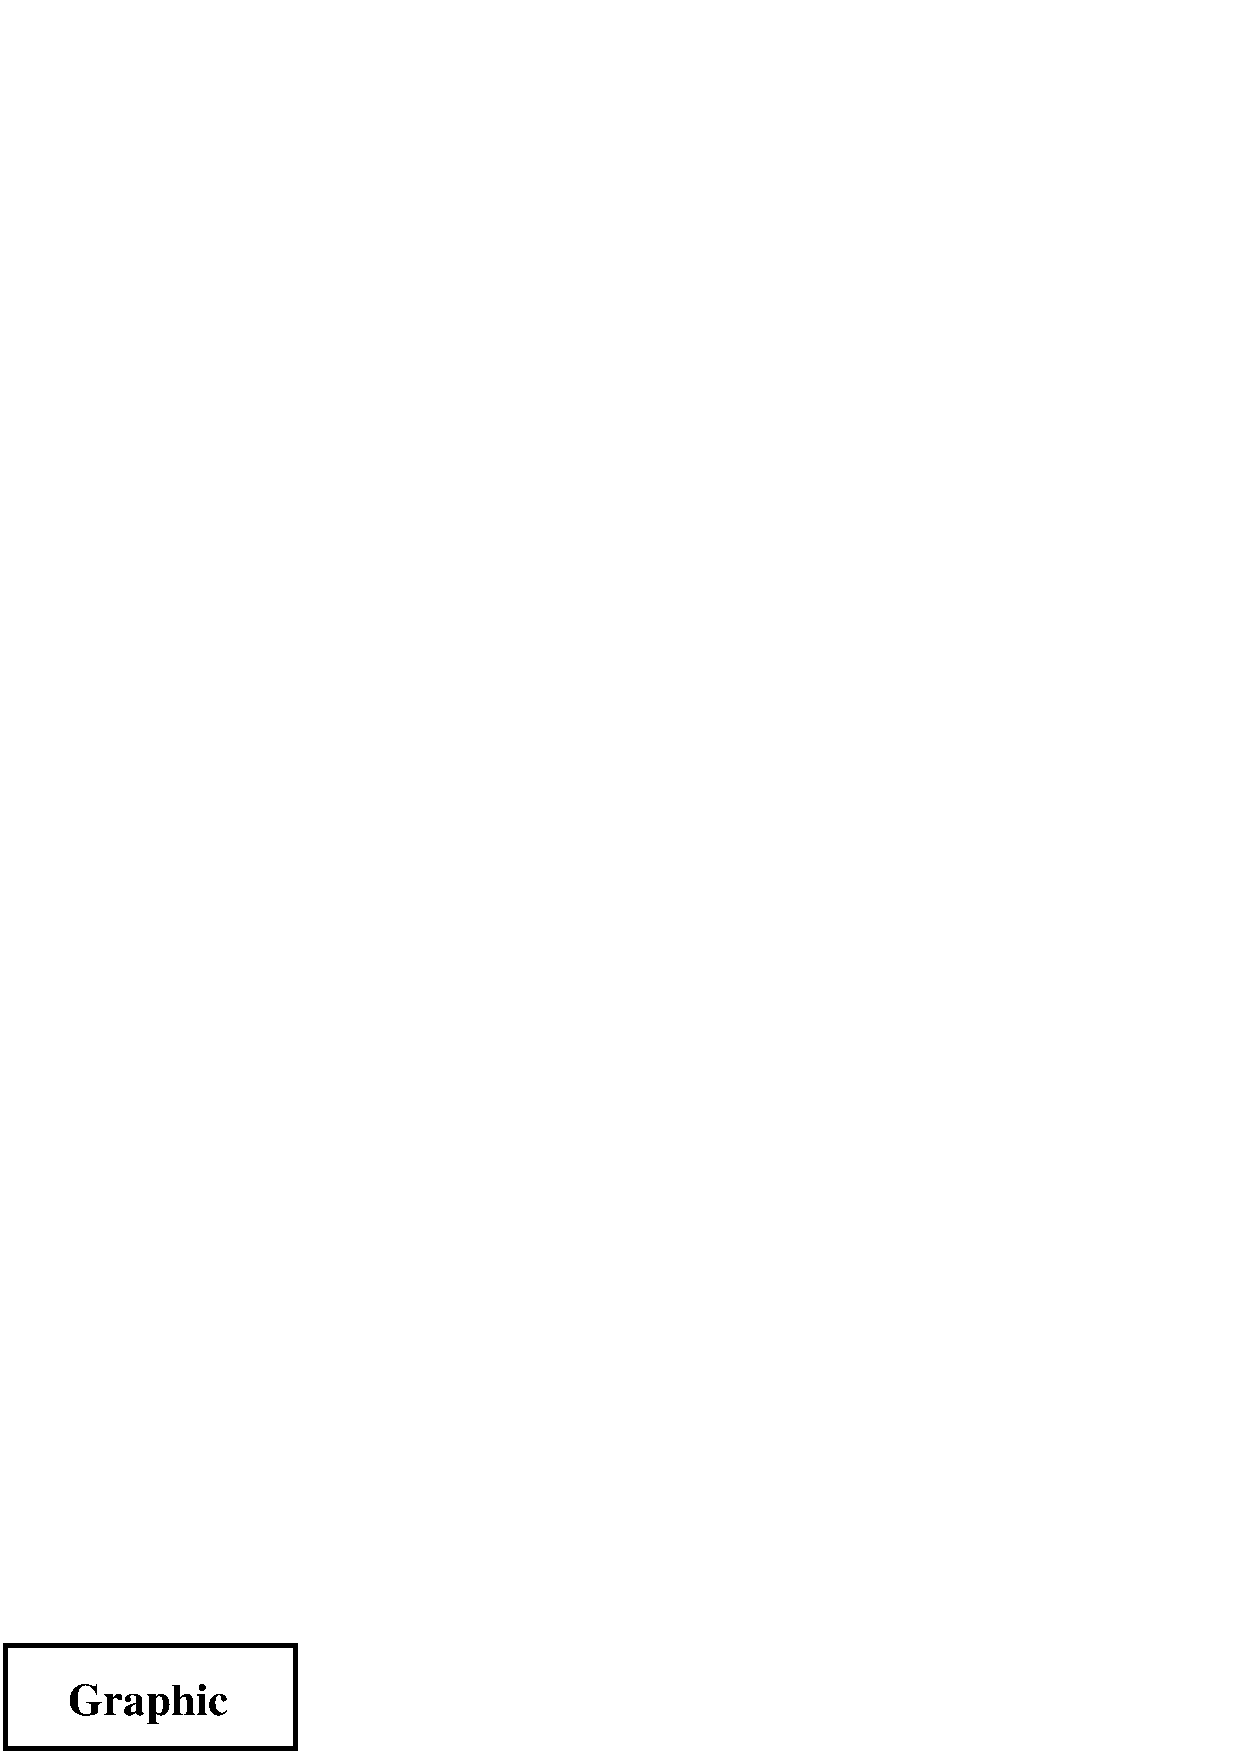
\includegraphics[width=0.25\linewidth]{graphic}}
	\hspace{0.1\linewidth}
	%%----start of second subfigure----
	\subfloat[Second Subfigure]{
		\label{fig:stacksub:b} %% label for second subfigure
		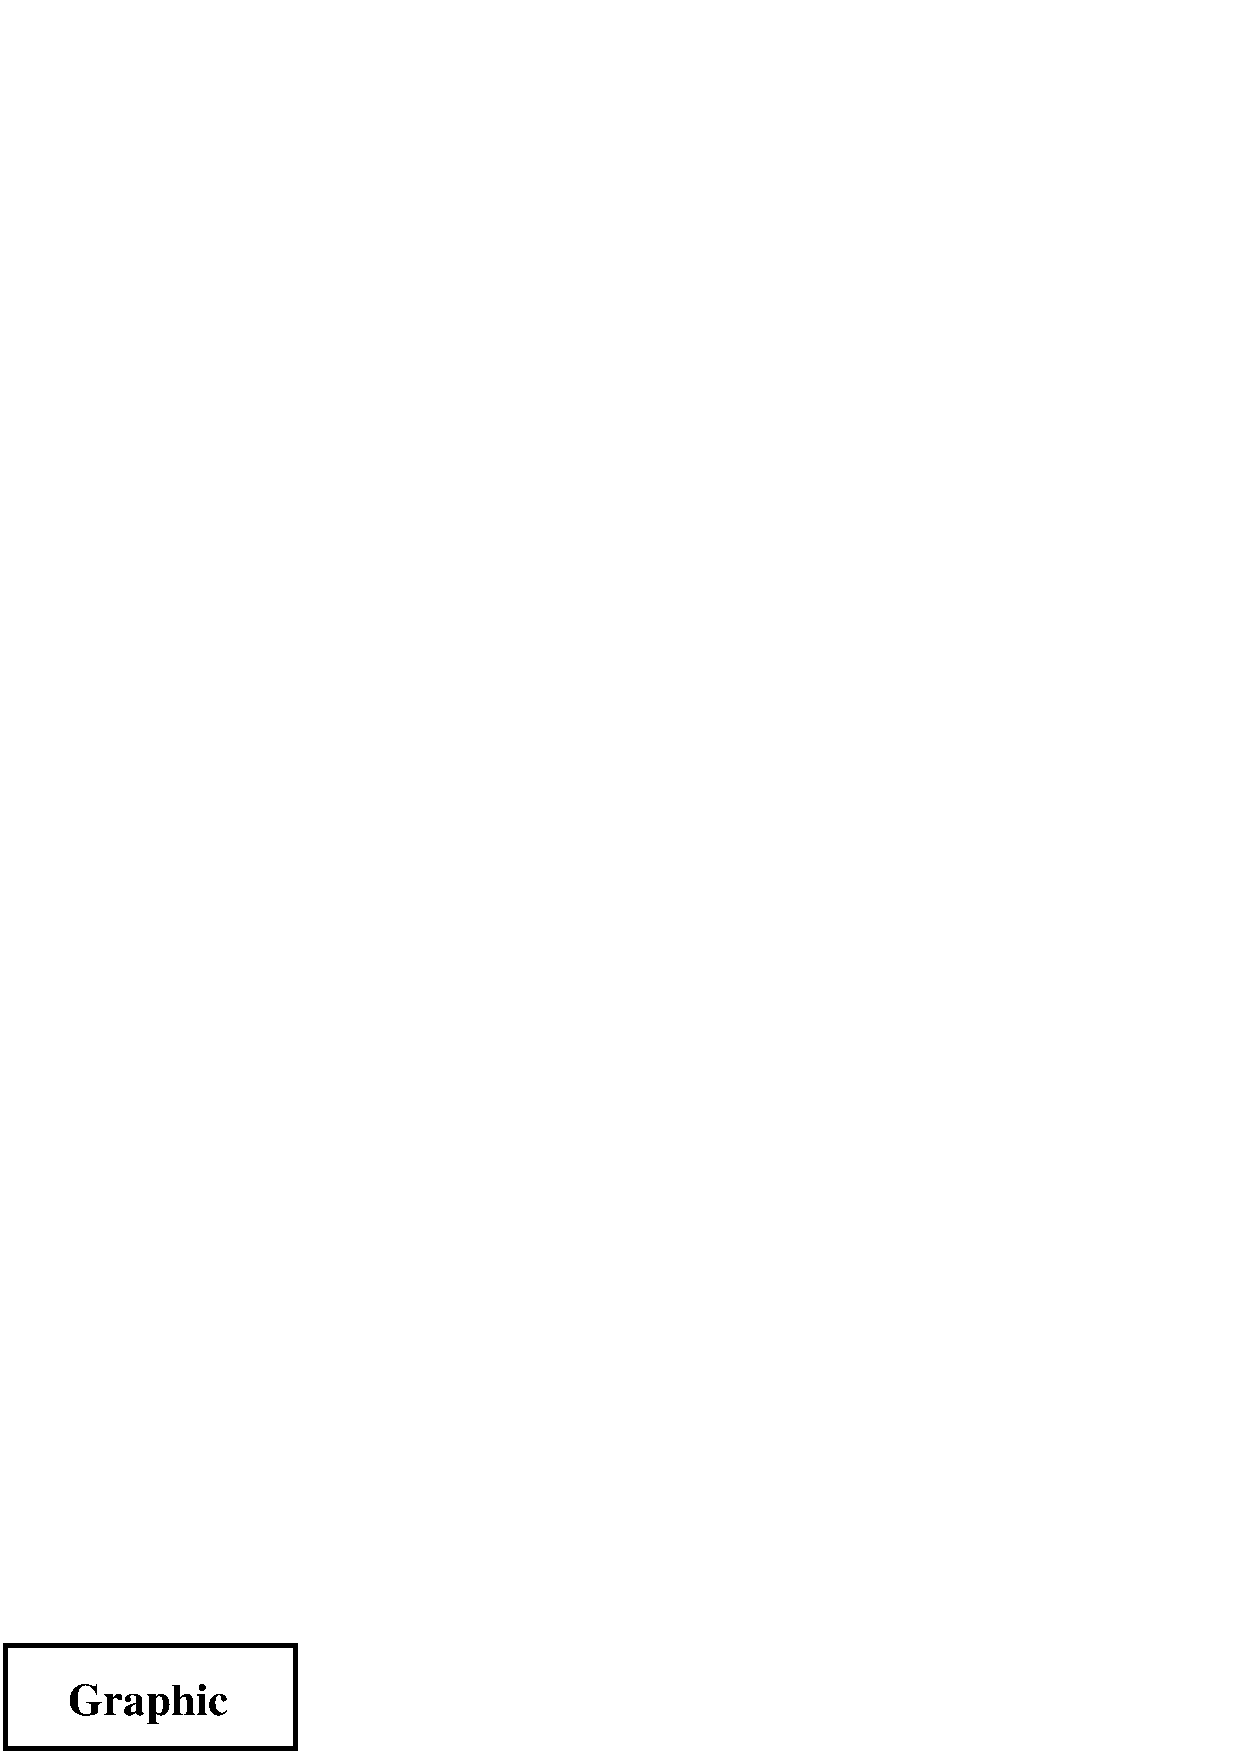
\includegraphics[width=0.25\linewidth]{graphic}}\\[20pt]
	%%----start of third subfigure----
	\subfloat[Third Subfigure]{
		\label{fig:stacksub:c} %% label for third subfigure
		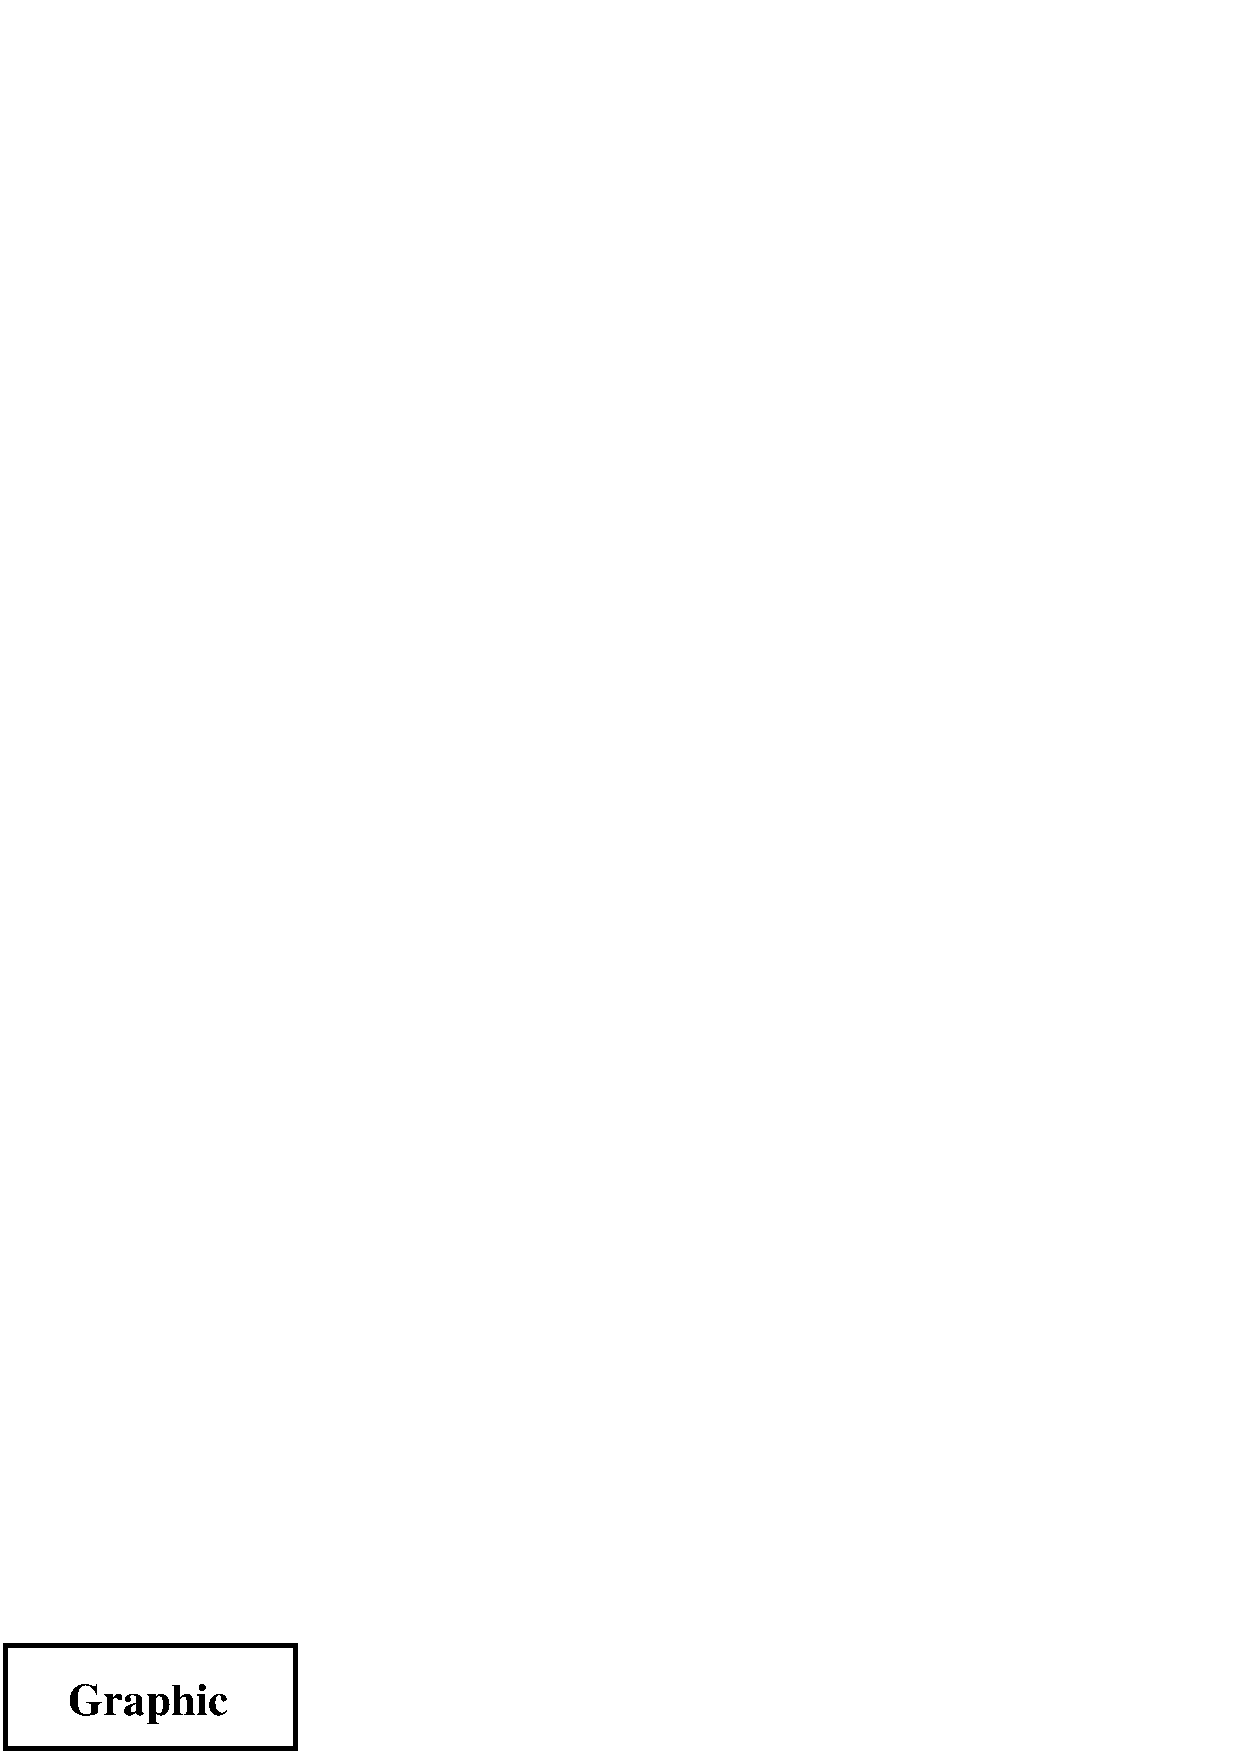
\includegraphics[width=0.25\linewidth]{graphic}}
	\hspace{0.1\linewidth}
	%%----start of fourth subfigure----
	\subfloat[Fourth Subfigure]{
		\label{fig:stacksub:d} %% label for fourth subfigure
		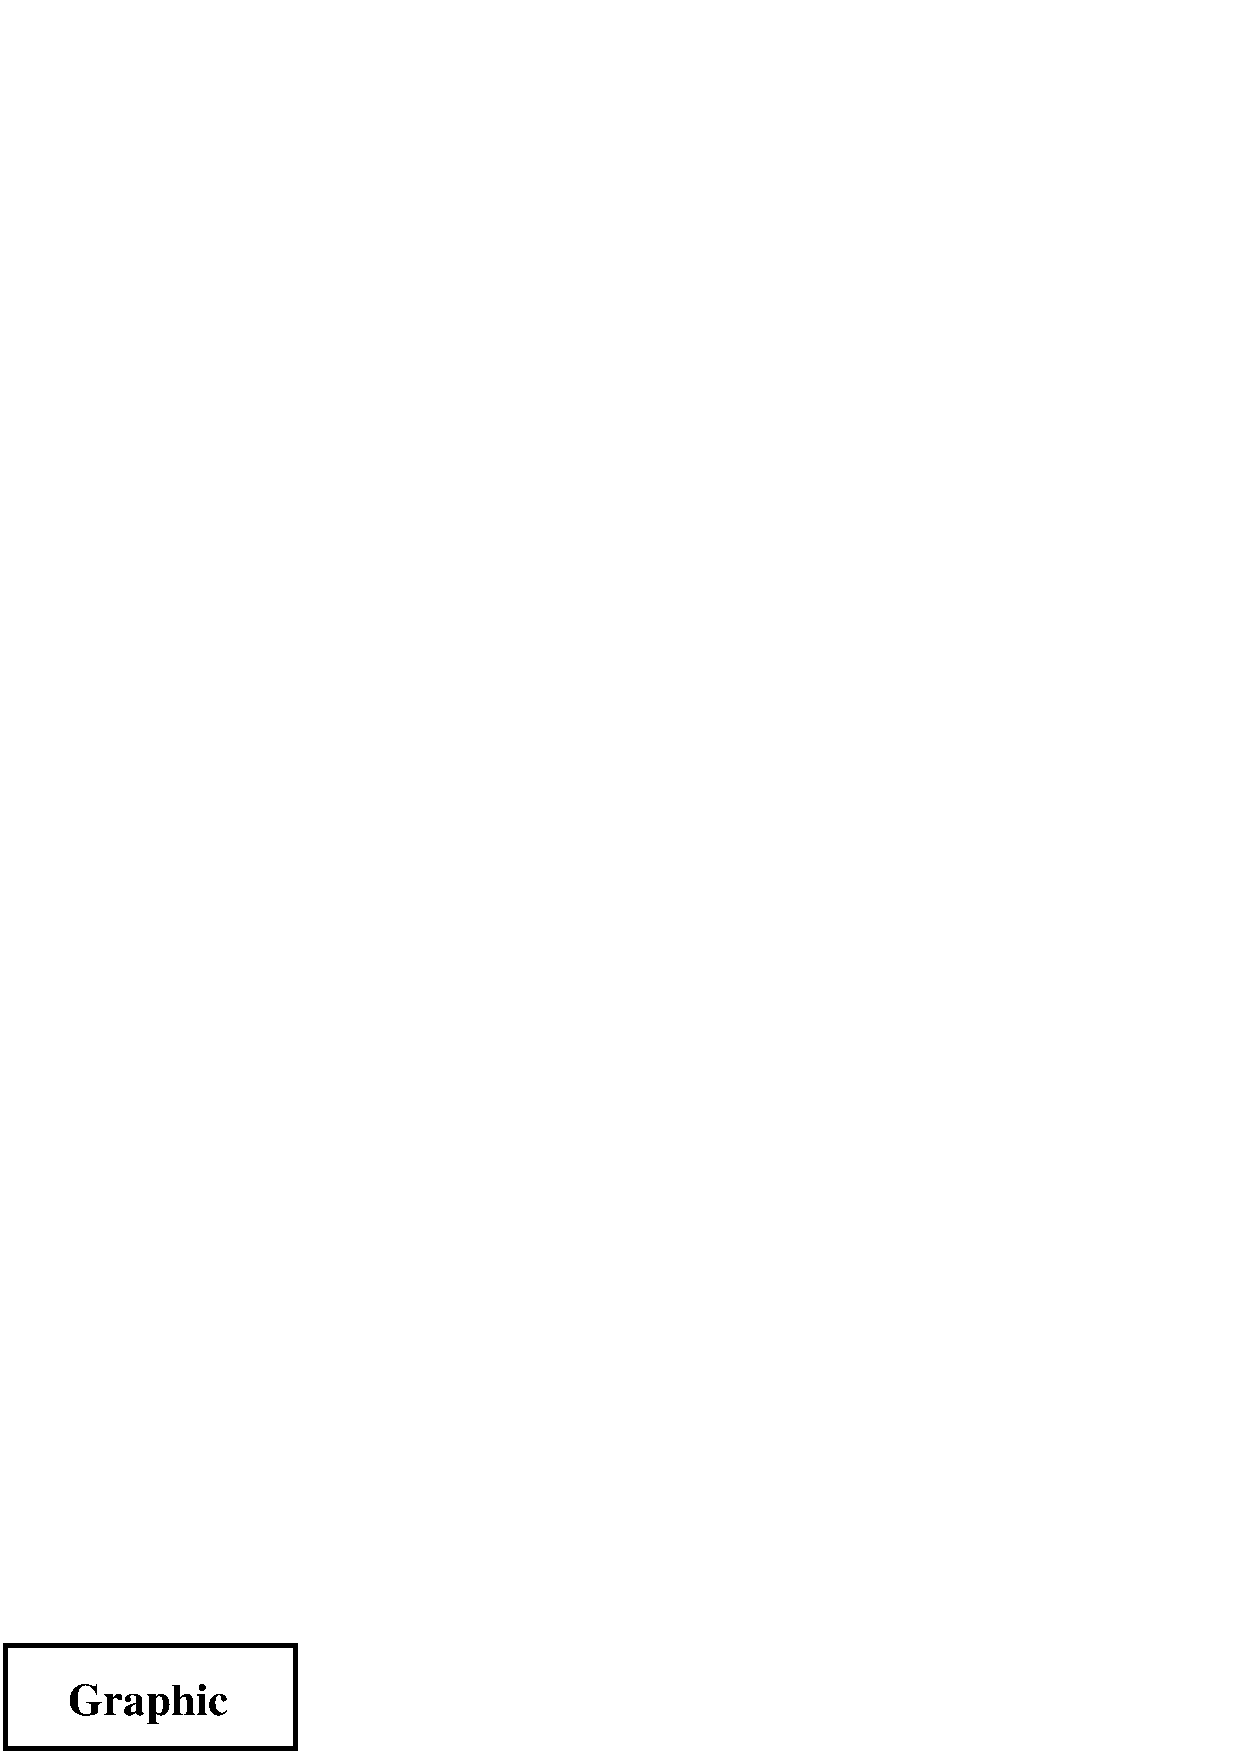
\includegraphics[width=0.25\linewidth]{graphic}}
	\hspace{0.1\linewidth}
	%%----start of fifth subfigure----
	\subfloat[Fifth Subfigure]{
		\label{fig:stacksub:e} %% label for fifth subfigure
		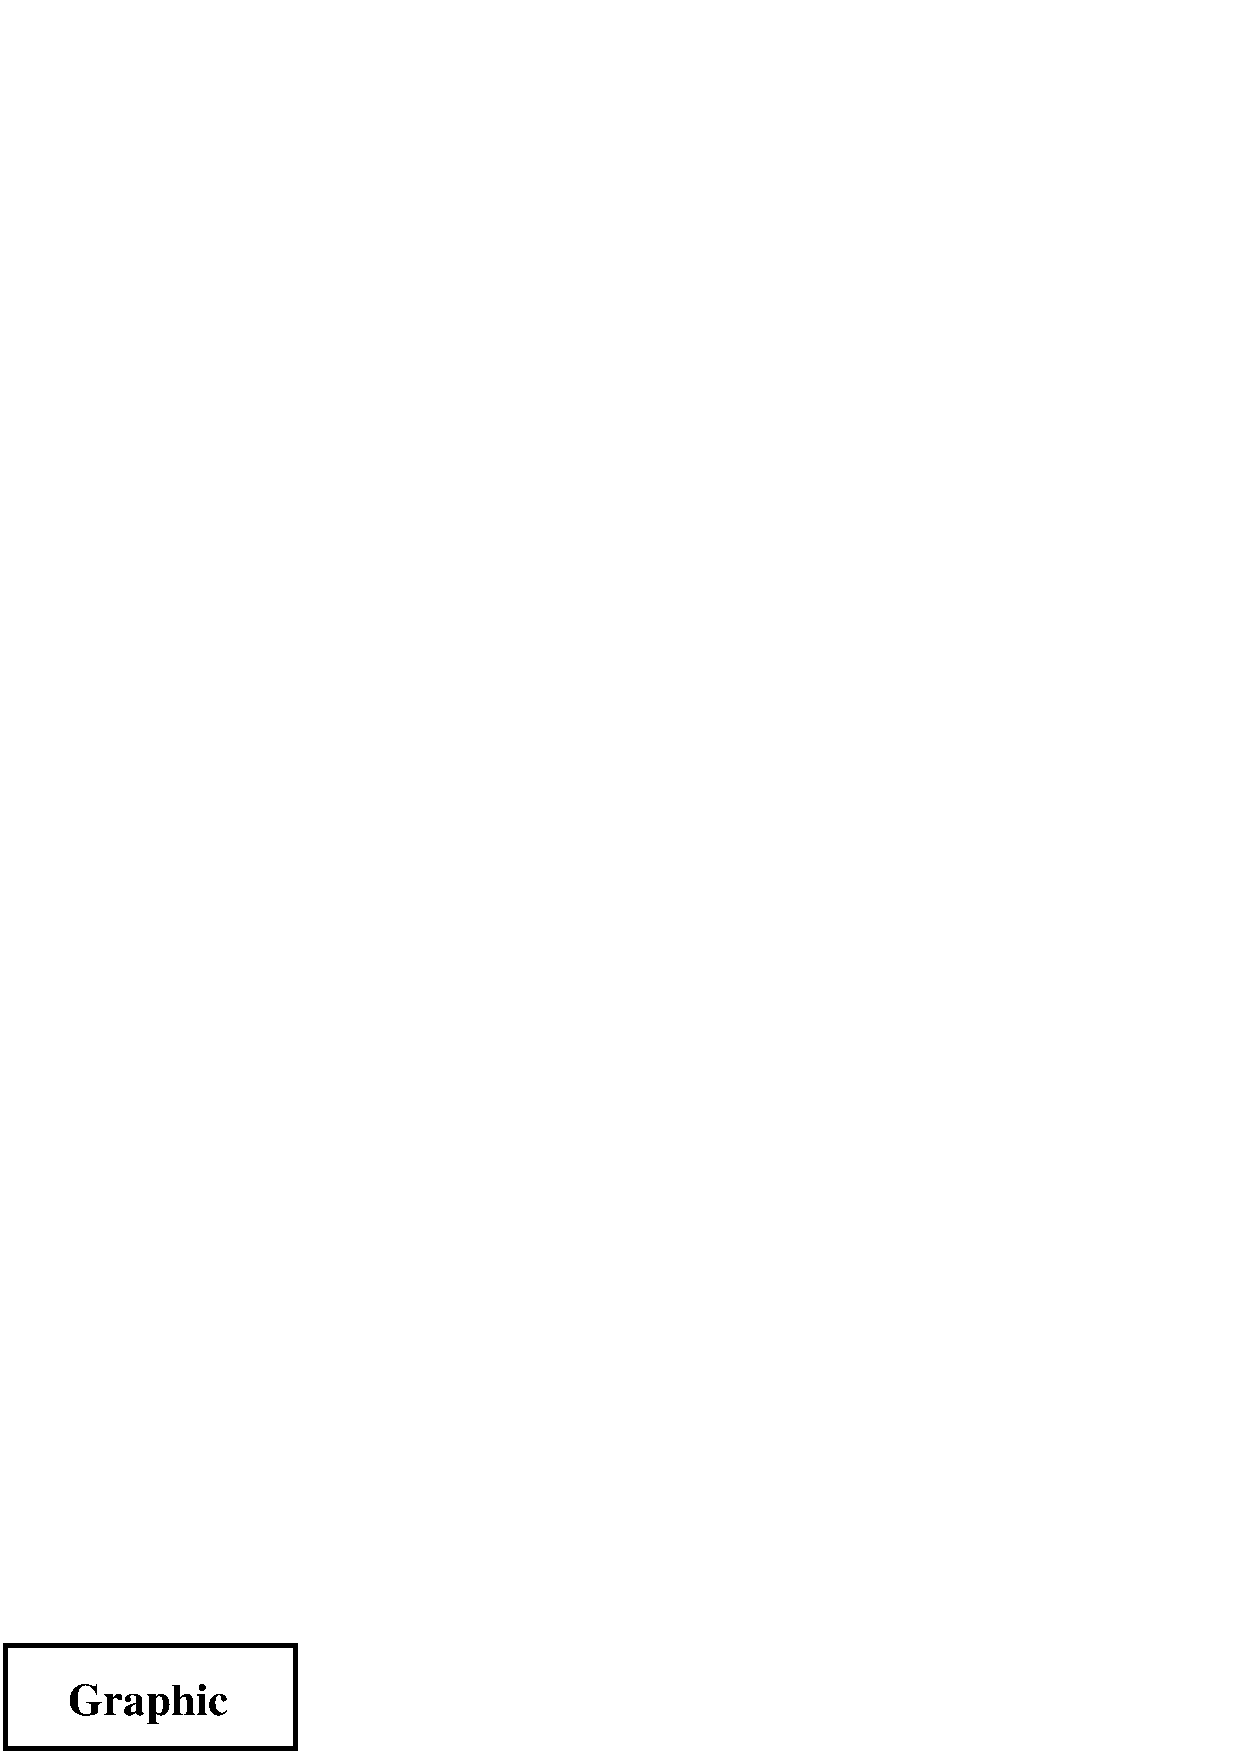
\includegraphics[width=0.25\linewidth]{graphic}}
	\caption{Five Subfigures}
	\label{fig:stacksub} %% label for entire figure
\end{figure}
\end{lstlisting}
生成图~\ref{fig:stacksub}。

\begin{figure}
	\centering
	%%----start of first subfigure----
	\subfloat[First Subfigure]{
		\label{fig:stacksub:a} %% label for first subfigure
		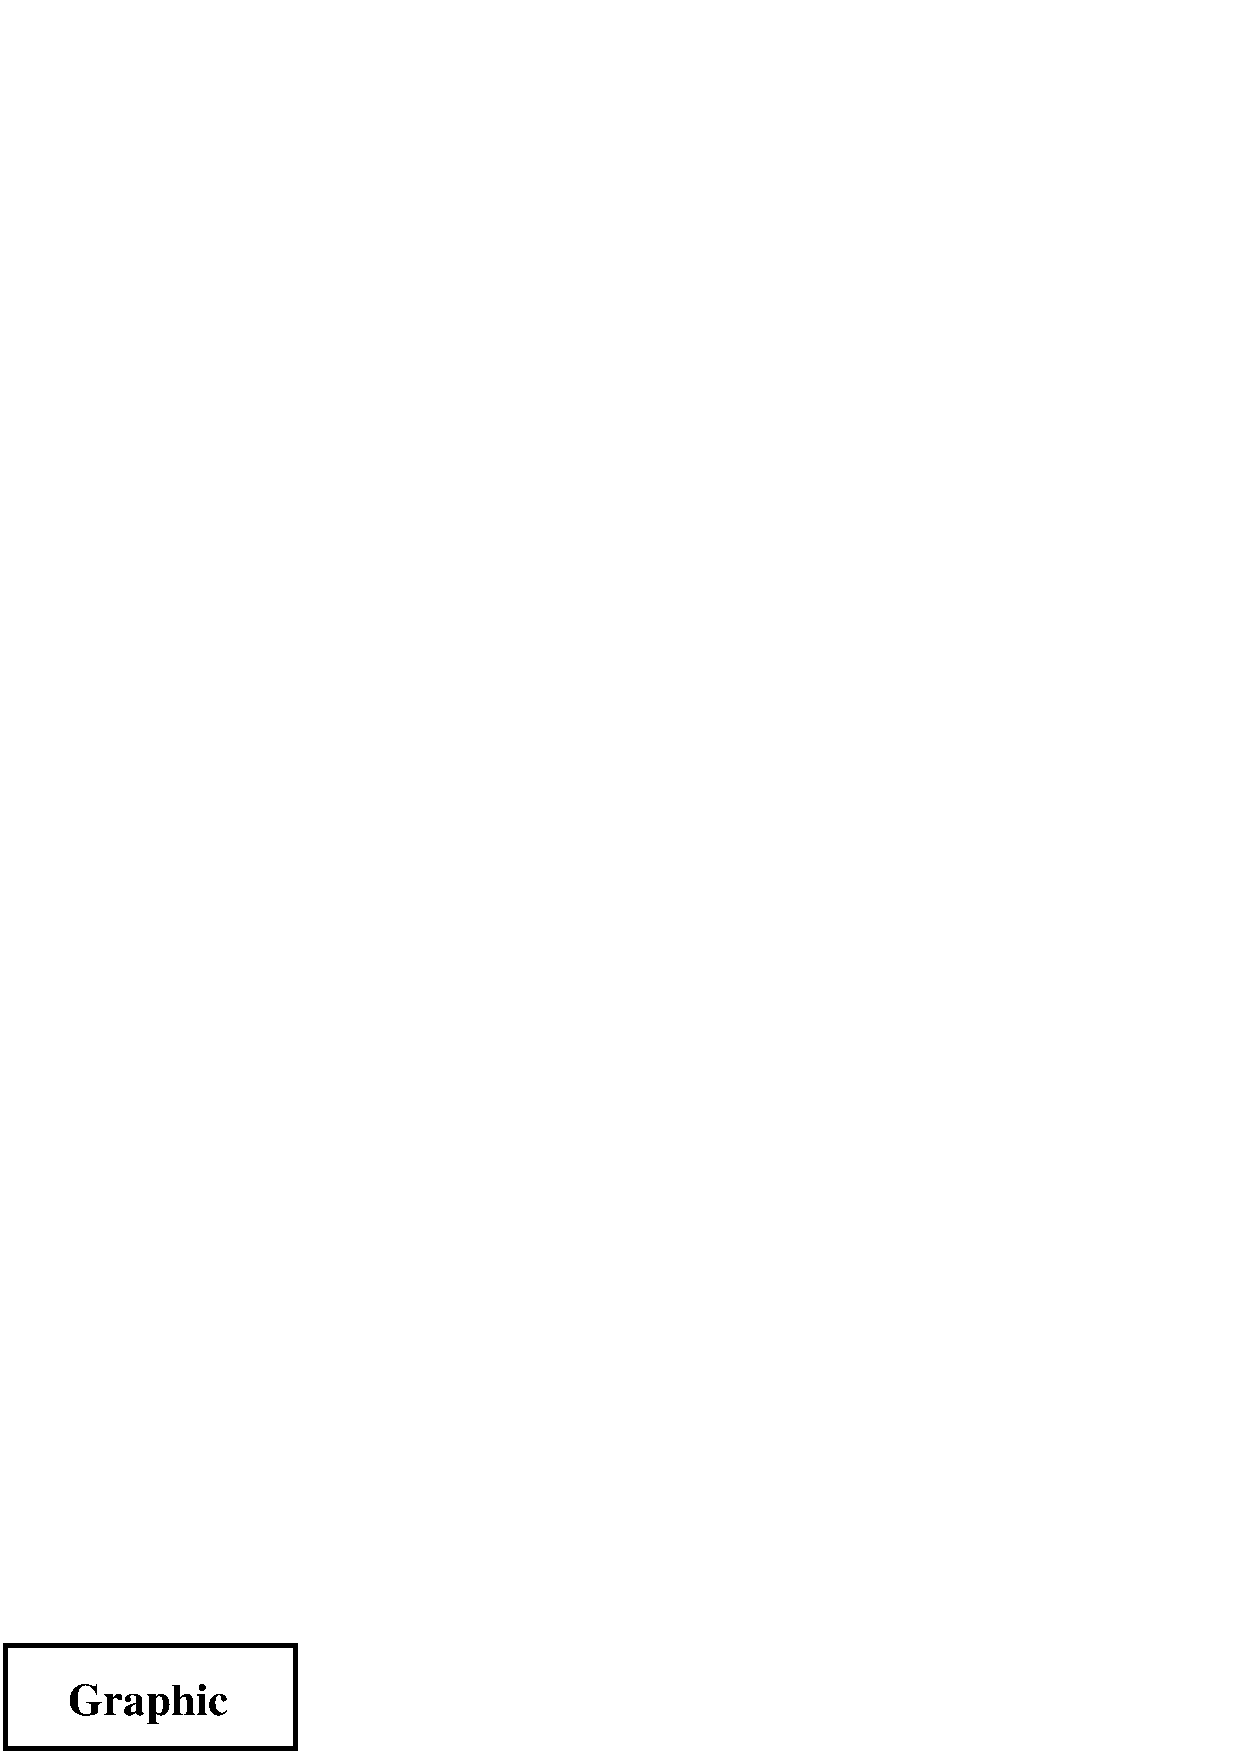
\includegraphics[width=0.25\linewidth]{graphic}}
	\hspace{0.1\linewidth}
	%%----start of second subfigure----
	\subfloat[Second Subfigure]{
		\label{fig:stacksub:b} %% label for second subfigure
		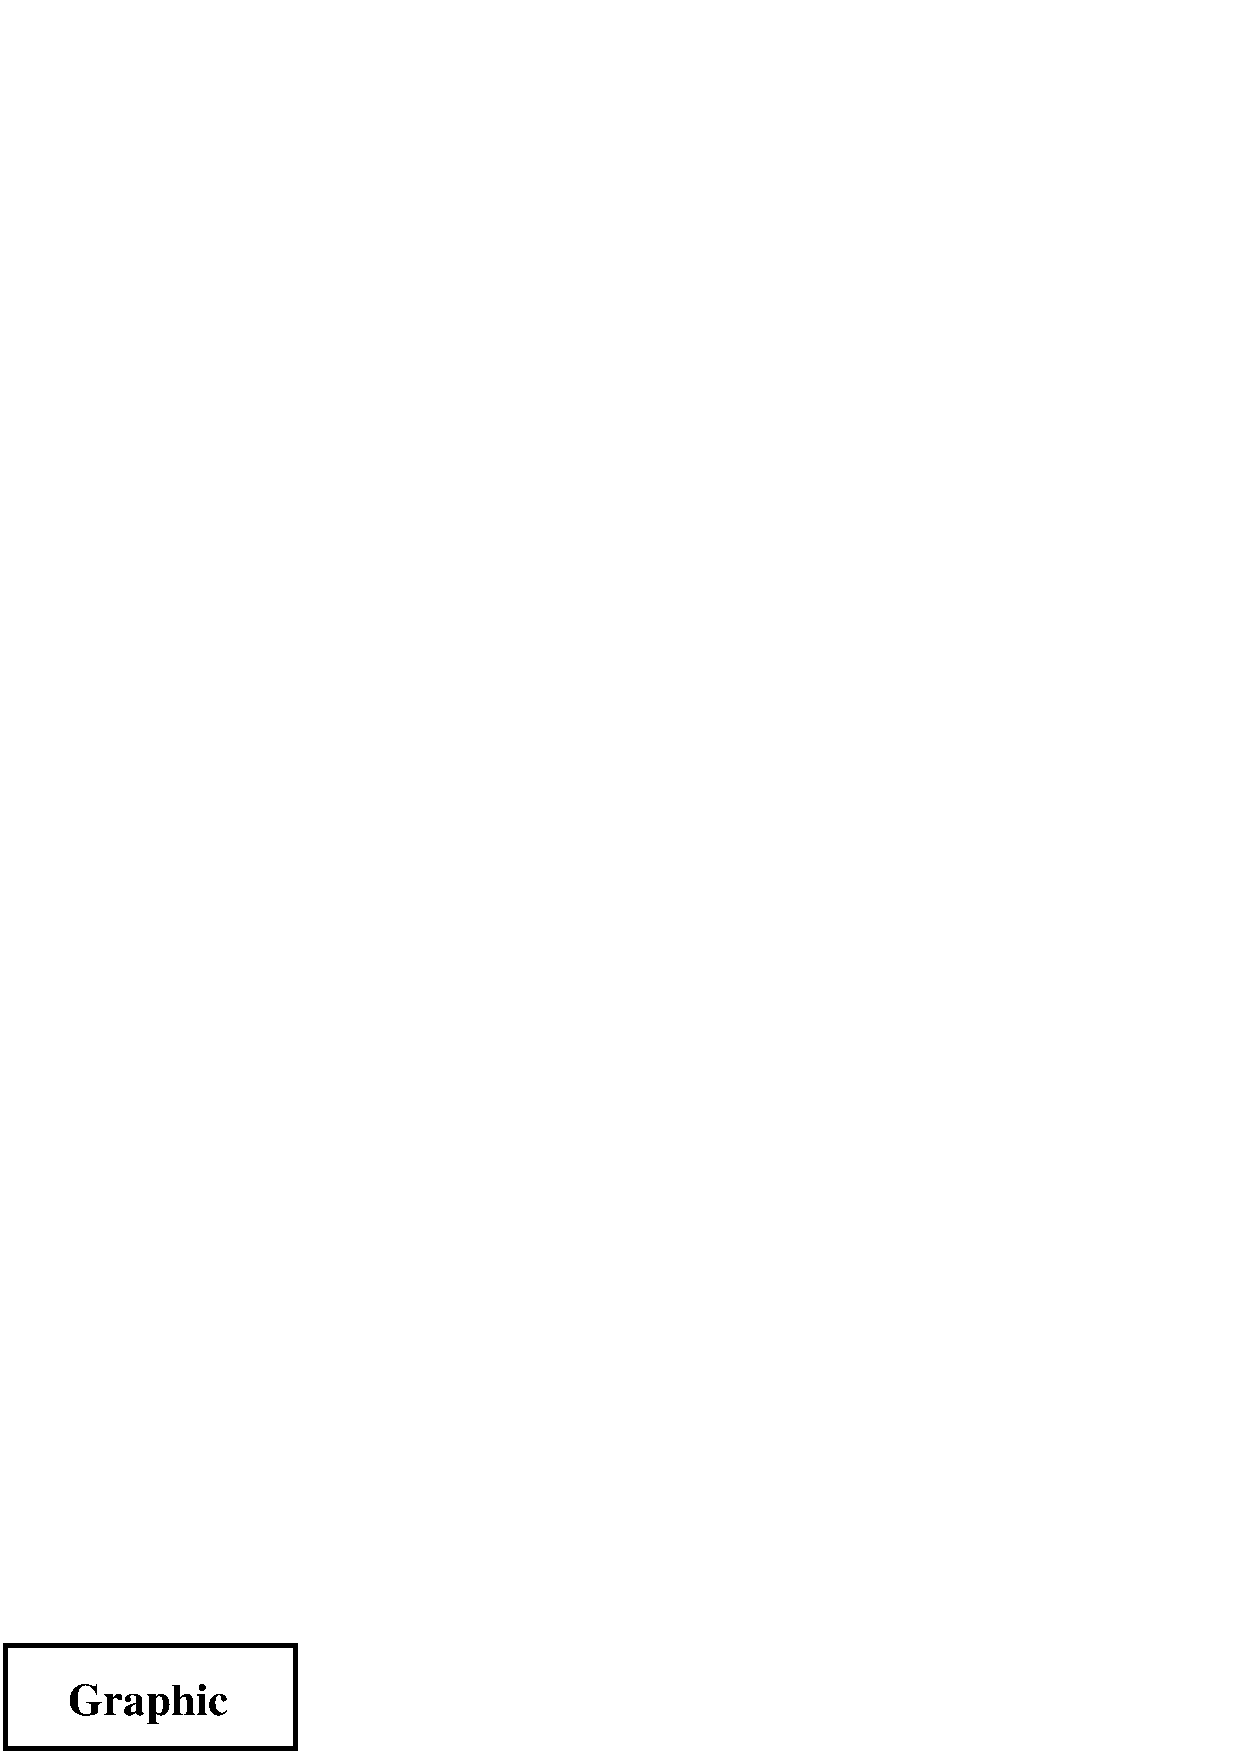
\includegraphics[width=0.25\linewidth]{graphic}}\\[20pt]
	%%----start of third subfigure----
	\subfloat[Third Subfigure]{
		\label{fig:stacksub:c} %% label for third subfigure
		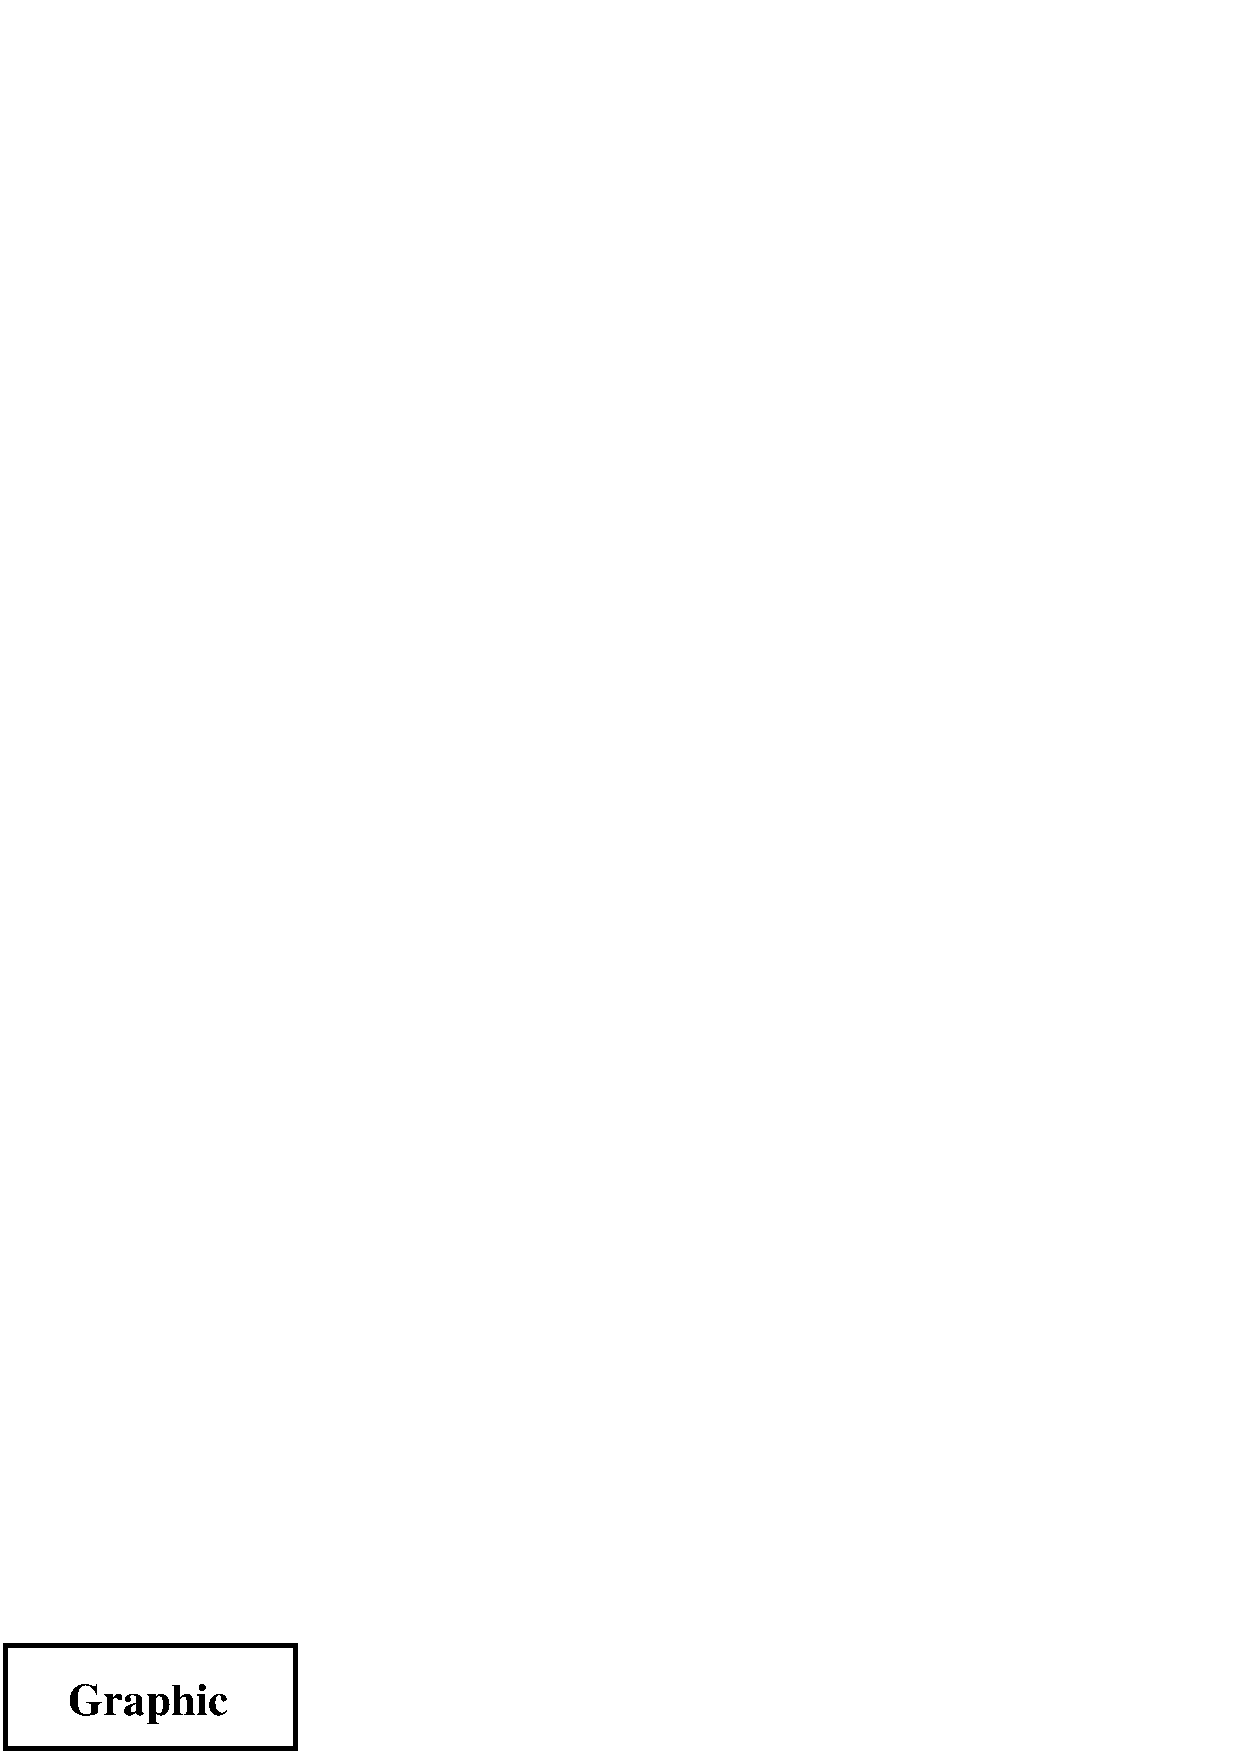
\includegraphics[width=0.25\linewidth]{graphic}}
	\hspace{0.1\linewidth}
	%%----start of fourth subfigure----
	\subfloat[Fourth Subfigure]{
		\label{fig:stacksub:d} %% label for fourth subfigure
		\includegraphics[width=0.25\linewidth]{graphic}}
	\hspace{0.1\linewidth}
	%%----start of fifth subfigure----
	\subfloat[Fifth Subfigure]{
		\label{fig:stacksub:e} %% label for fifth subfigure
		\includegraphics[width=0.25\linewidth]{graphic}}
	\caption{Five Subfigures}
	\label{fig:stacksub} %% label for entire figure
\end{figure}


\section{The subfig package}

\section{连续图形和连续子图}\label{sec:contfig}

当连续两个图形的内容关系较为密切时,常常希望具有相同的图形编号。
因为计数器 \opt{figure} 中记录了下一图形的编号,
所以可在图形环境前减小 \opt{figure} 的值使得两幅图形具有相同的编号。例如:
\begin{lstlisting}
\begin{figure}
....
\end{figure}
\addtocounter{figure}{-1}
\begin{figure}
....
\end{figure}
\end{lstlisting}
不过,这样做会使得两幅图形无法被正确区分,导致 \LaTeX{} 的引用的混乱。

\subsection{连续图形}

连续图形既需要具有相同的编号,又应该有各自不同的引用,例如“Figure 12, Figure 12b”。
构造连续图形的最佳办法是使用 \pkg{caption} 宏包。
\pkg{caption} 宏包提供了 \cmdi{ContinuedFloat} 命令以及相应的标题类型 \opt{ContinuedFloat} 以及同名的计数器 \opt{ContinuedFloat}。
\begin{lstlisting}
\renewcommand\theContinuedFloat{\alph{ContinuedFloat}}
\DeclareCaptionLabelFormat{continued}{Continued #1˜#2}
\captionsetup[ContinuedFloat]{labelformat=continued}
...
\begin{figure}
	...
	\caption{A figure}
\end{figure}
...
\begin{figure}\ContinuedFloat
	...
	\caption{A figure}
\end{figure}
\end{lstlisting}

更多情况下希望第一幅图从“Figure 12a”而不是“Figure 12”开始,
进而第二幅图是“Figure 12b”而不是“Figure 12a”。
此时需要在第一幅图的环境内使用 \cmdi{ContinuedFloat*} 命令。
\begin{lstlisting}
\renewcommand\theContinuedFloat{\alph{ContinuedFloat}}
...
\begin{figure}[tbp]
	\ContinuedFloat*
	\centering
	\includegraphics[height=6in]{tux-color}
	\caption{First figure of a series}
	\label{fig:continued:first}
\end{figure}
...
\begin{figure}[tbp]
	\ContinuedFloat
	\centering
	\includegraphics[height=6in]{tux-black}
	\caption{Second figure of a series}
	\label{fig:continued:second}
\end{figure}
\end{lstlisting}
效果见图~\ref{fig:continued:first} 和图~\ref{fig:continued:second}。

\begin{figure}[tbp]
	\ContinuedFloat*
	\centering
	\includegraphics[height=6in]{tux-color}
	\caption{First figure of a series}
	\label{fig:continued:first}
\end{figure}

\begin{figure}[tbp]
	\ContinuedFloat
	\centering
	\includegraphics[height=6in]{tux-black}
	\caption{Second figure of a series}
	\label{fig:continued:second}
\end{figure}

\subsection{连续子图}

当一个 \env{figure} 环境中包含很多子图时,
很多时候没有足够的空间将所有的子图放在一页内。
此时使用 \cmd{ContinuedFloat} 命令可以使子图分成若干组,并且具有相同的图形编号。
这样就可以避免分割在不同编号的图形环境。

\begin{lstlisting}
\usepackage{graphicx}
\usepackage{caption,subcaption}
...
\begin{figure}
	\centering
	%%----start of first subfigure----
	\subcaptionbox{%
		First Subfigure\label{fig:contfig:subone}}{%
		\includegraphics[width=3cm]{graphic}}
	\hspace{1cm}
	%%----start of second subfigure----
	\subcaptionbox{%
		Second Subfigure\label{fig:contfig:subtwo}}{%
		\includegraphics[width=3cm]{graphic}}
	\caption{Two Subfigures}
	\label{fig:contfig:one}
\end{figure}
\begin{figure}
	\ContinuedFloat
	\centering
	%%----start of third subfigure----
	\subcaptionbox{%
		Third Subfigure\label{fig:contfig:subthree}}{%
		\includegraphics[width=3cm]{graphic}}
	\hspace{1cm}
	%%----start of fourth subfigure----
	\subcaptionbox{%
		Fourth Subfigure\label{fig:contfig:subfour}}{%
		\includegraphics[width=3cm]{graphic}}
	\caption{Two Additional Subfigures}
	\label{fig:contfig:two}
\end{figure}
\end{lstlisting}
该代码片段会创建两个浮动体,
分别包含图~\ref{fig:contfig:subone}、\ref{fig:contfig:subtwo} 
以及图~\ref{fig:contfig:subthree}、\ref{fig:contfig:subfour}。
显然这四个子图可以放在同一个浮动体内,
但本例只是为了说明如何进行更大的子图分组。

注意 \cmd{ContinuedFloat} 命令不仅保持浮动体编号不变,而且确保第二个浮动体内的子图编号不会重置为 (a)。
此外两个浮动体的标题具有不同的引用标签(\texttt{fig:contfig:one} 和 \texttt{fig:contfig:two}),
但相应的 \cmd{ref} 引用值是相同的,
不过由于两个浮动体可能不同页,因此对应的 \cmd{pageref} 值可能不同。

\begin{figure}
	\centering
	%%----start of first subfigure----
	\subcaptionbox{%
		First Subfigure\label{fig:contfig:subone}}{%
		\includegraphics[width=3cm]{graphic}}
	\hspace{1cm}
	%%----start of second subfigure----
	\subcaptionbox{%
		Second Subfigure\label{fig:contfig:subtwo}}{%
		\includegraphics[width=3cm]{graphic}}
	\caption{Two Subfigures}
	\label{fig:contfig:one}
\end{figure}
\begin{figure}
	\ContinuedFloat
	\centering
	%%----start of third subfigure----
	\subcaptionbox{%
		Third Subfigure\label{fig:contfig:subthree}}{%
		\includegraphics[width=3cm]{graphic}}
	\hspace{1cm}
	%%----start of fourth subfigure----
	\subcaptionbox{%
		Fourth Subfigure\label{fig:contfig:subfour}}{%
		\includegraphics[width=3cm]{graphic}}
	\caption{Two Additional Subfigures}
	\label{fig:contfig:two}
\end{figure}

\endinput
